%# -*- coding: utf-8-unix -*-
%%==================================================
%% thesis.tex
%%==================================================

% 双面打印
\documentclass[master, fontset=none, openright, twoside,review,zihao=-4]{sjtuthesis}
%\documentclass[master, fontset=none, openright, twoside,submit,zihao=-4]{sjtuthesis}

% \documentclass[bachelor, fontset=adobe, openany, oneside, submit]{sjtuthesis} 
% \documentclass[master, adobefonts, review]{sjtuthesis} 
% \documentclass[%
%   bachelor|master|doctor,	% 必选项
%   fontset=adobe|windows,  	% 只测试了adobe
%   oneside|twoside,		% 单面打印,双面打印(奇偶页交换页边距,默认)
%   openany|openright, 		% 可以在奇数或者偶数页开新章|只在奇数页开新章(默认)
%   zihao=-4|5, 		% 正文字号:小四、五号(默认)
%   review,	 		% 盲审论文,隐去作者姓名、学号、导师姓名、致谢、发表论文和参与的项目
%   submit			% 定稿提交的论文,插入签名扫描版的原创性声明、授权声明 
% ]

%% font settings
\usepackage{thesisfonts_external}
\usepackage[square,numbers,sort&compress]{natbib}
\usepackage[nottoc]{tocbibind}
% 逐个导入参考文献数据库
%\addbibresource{bib/thesis.bib}

% \addbibresource{bib/chap2.bib}

\begin{document}

%% 无编号内容:中英文论文封面、授权页
%# -*- coding: utf-8-unix -*-
\title{机票个性化推荐的研究与探索}
\author{某\quad{}某}
\advisor{某某}
\defenddate{2014年12月17日}
\school{上海交通大学}
\institute{某某系}
\studentnumber{0010900990}
\major{某某专业}

\englishtitle{Research of Personalized Flight Recommendation}
\englishauthor{\textsc{Mo Mo}}
\englishadvisor{Prof. \textsc{Mou Mou}}
% \englishcoadvisor{Prof. \textsc{Uom Uom}}
\englishschool{Shanghai Jiao Tong University}
\englishinstitute{\textsc{Depart of XXX, School of XXX} \\
  \textsc{Shanghai Jiao Tong University} \\
  \textsc{Shanghai, P.R.China}}
\englishmajor{A Very Important Major}
\englishdate{Dec. 17th, 2014}


\maketitle

\makeenglishtitle

\makeatletter
\ifsjtu@submit\relax
	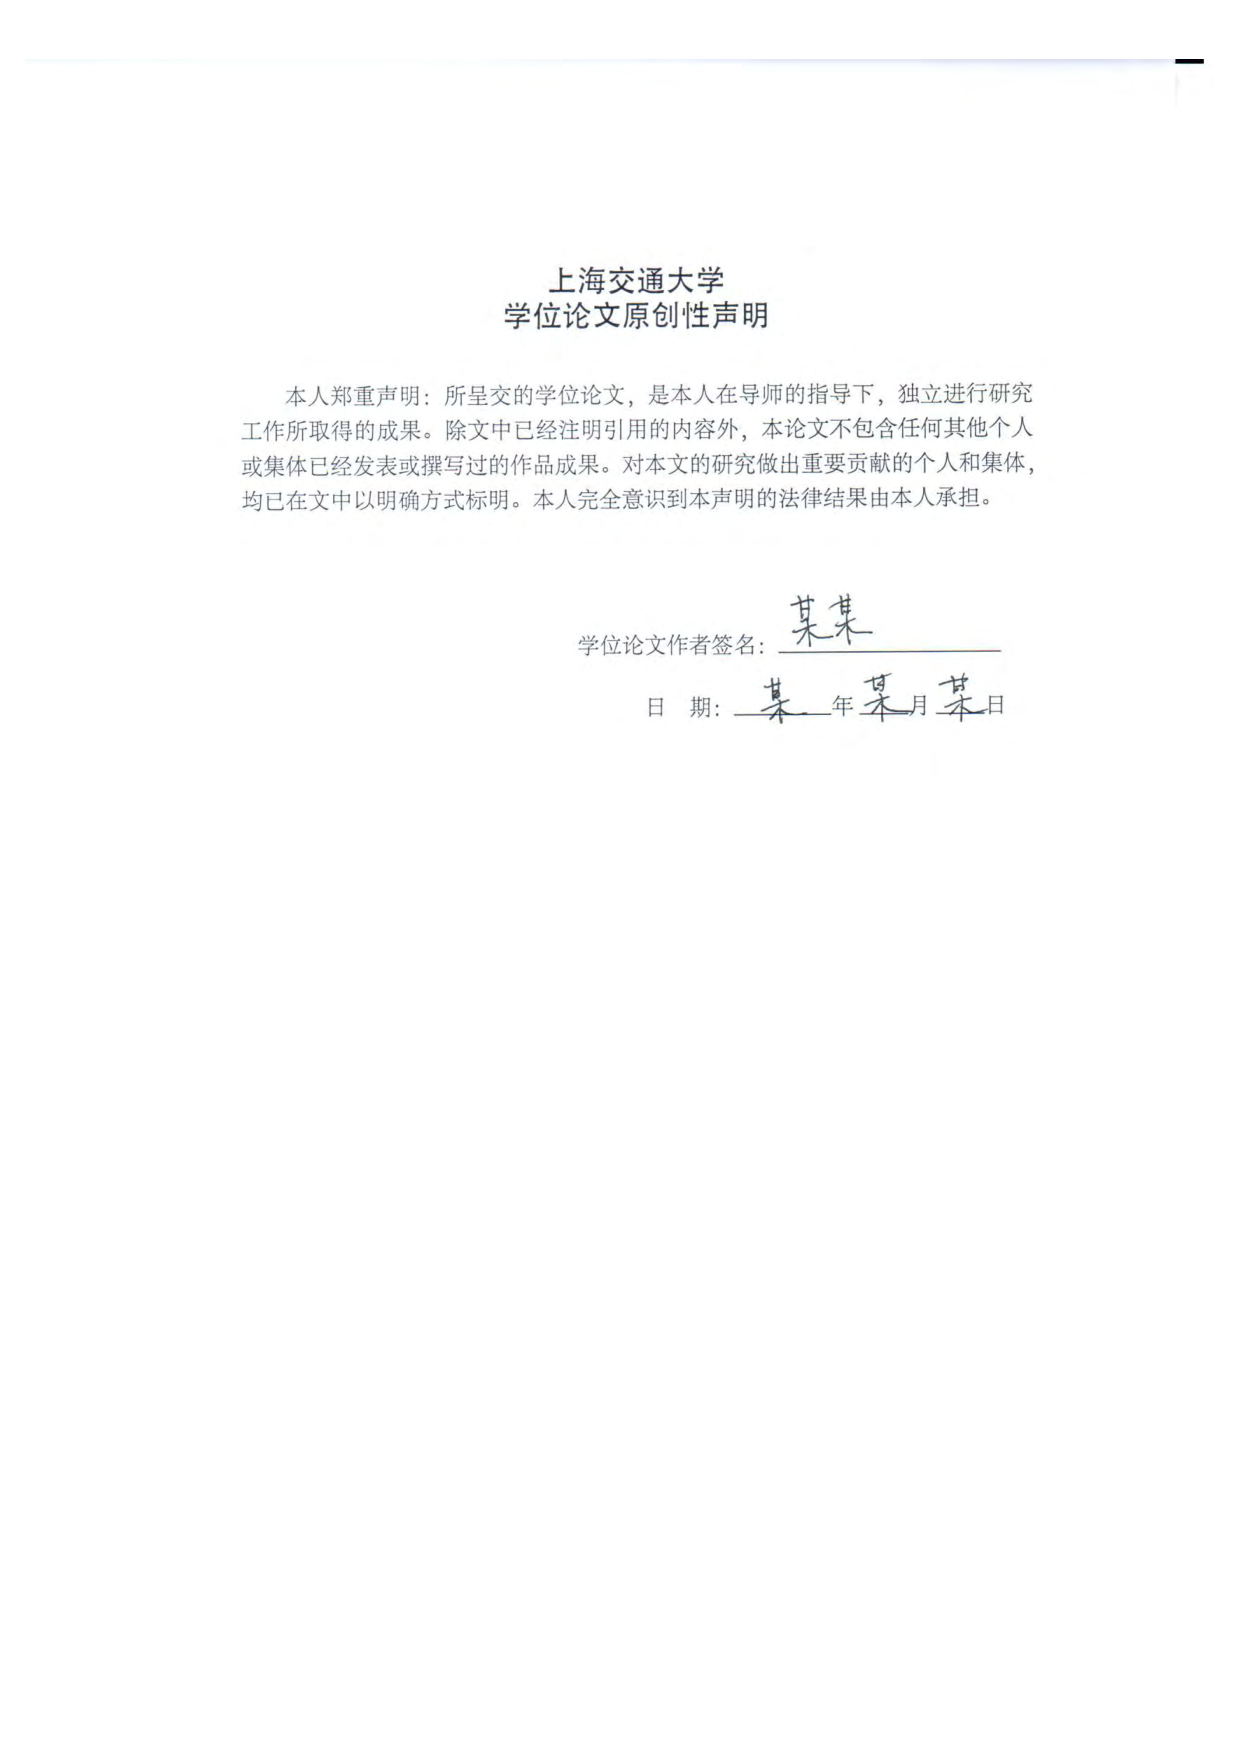
\includepdf{pdf/original.pdf}
	\cleardoublepage
	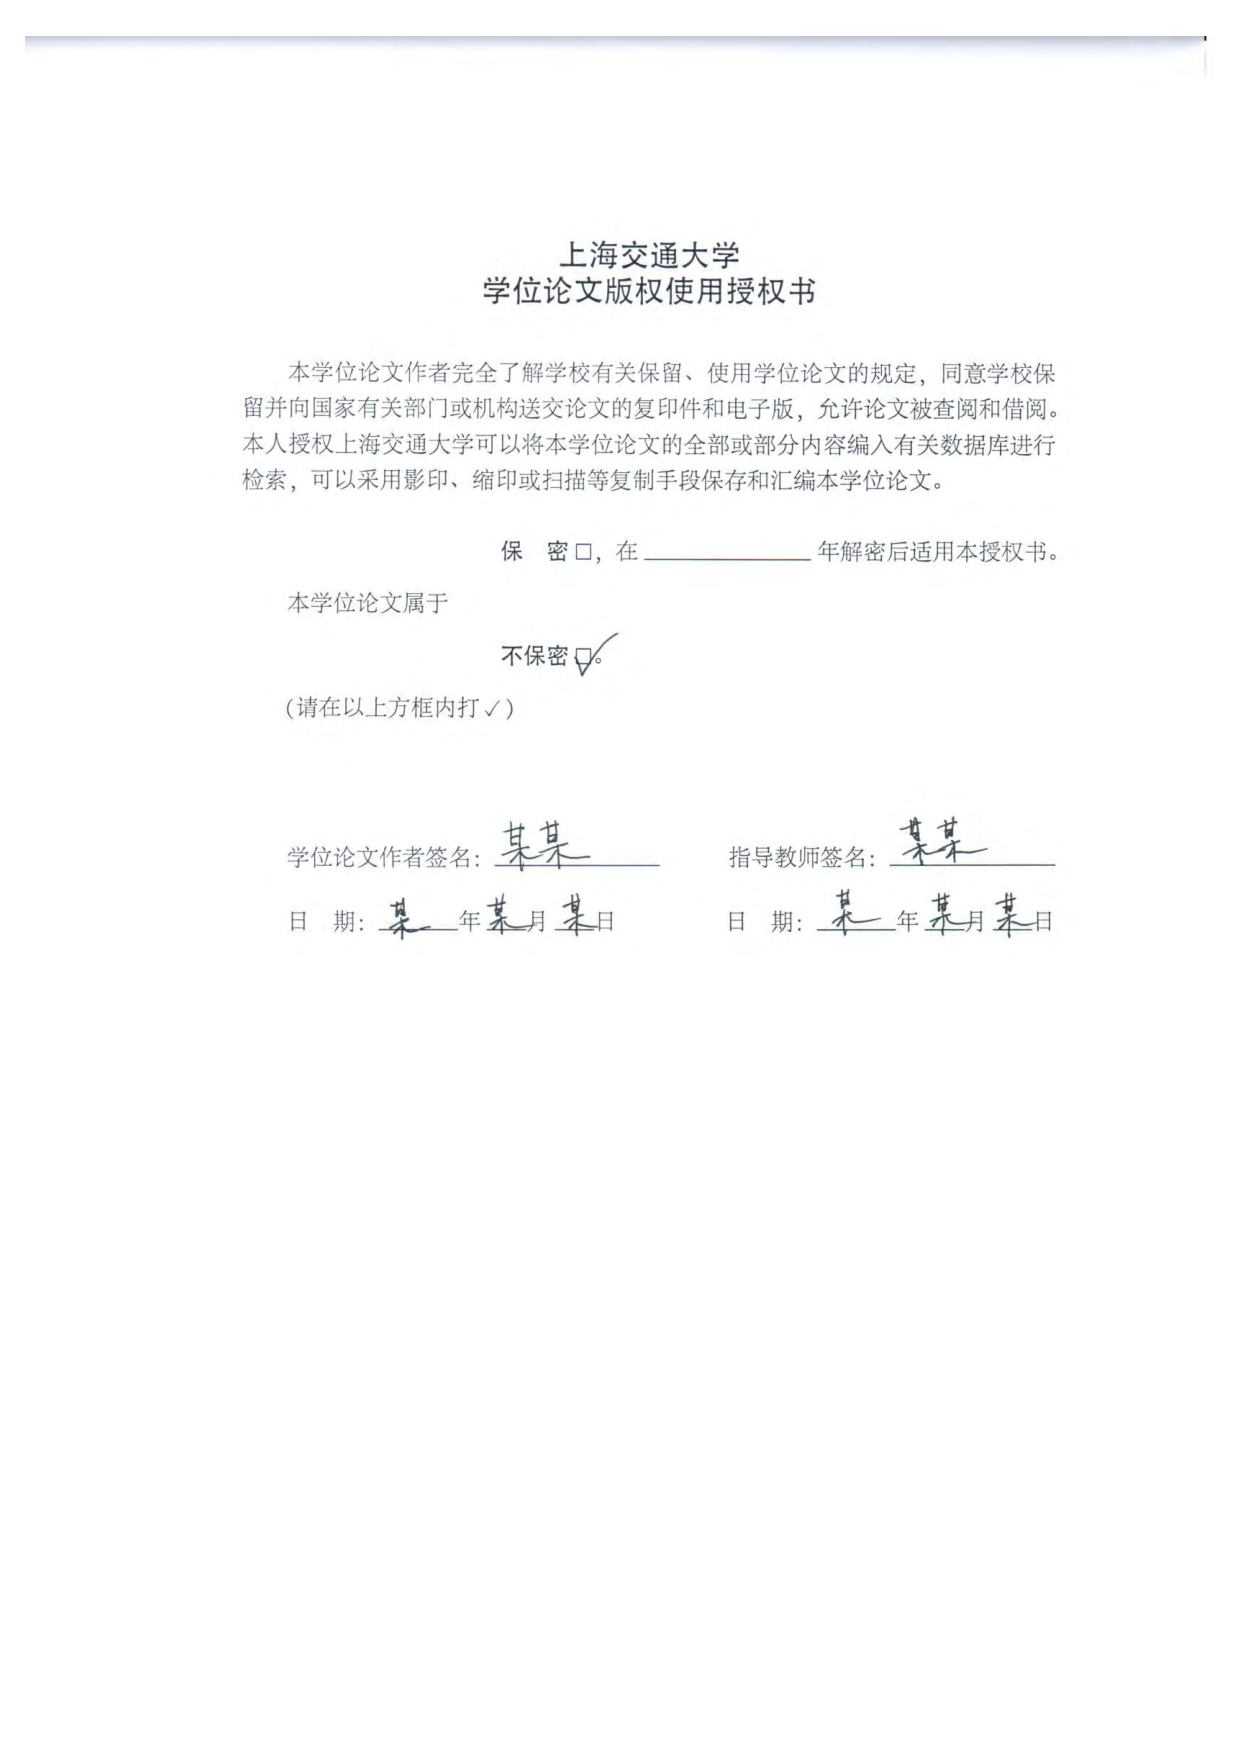
\includepdf{pdf/authorization.pdf}
	\cleardoublepage
\else
	\makeDeclareOriginal
	\makeDeclareAuthorization
\fi
\makeatother


\frontmatter 	% 使用罗马数字对前言编号

%% 摘要
\pagestyle{main}
\begin{abstract}
\addcontentsline{toc}{chapter}{摘要}
随着在线旅游业的发展,越来越多的用户通过在线票务网站订购机票。用户只需输入起飞城市、到达城市和起飞日期,就可以检索到所有航空公司提供的候选机票。虽然在线机票订购丰富了用户的选择,但对于很多航线,候选机票的数量很大,一定程度上增加了用户的选择成本,降低了用户体验。如果能够根据用户的偏好,为用户从候选机票中推荐满足其出行计划的机票,就可以克服机票订购过程中的信息过载问题。

本文对个性化机票推荐问题进行了研究。首先,我们根据机票的特征构建了用户特征分布模型,提出基于用户偏好的机票推荐算法。其后,针对机票推荐中仍存在的一些问题,细化了推荐场景,进一步提升机票推荐的效果。本文主要工作体现在以下几个方面:

1. 提出基于用户特征分布的机票推荐算法。结合数据分析与业务知识,对机票进行关键特征选取,提出了用户特征分布模型和基于该模型的机票推荐算法。本项工作作为深入研究的基础,贯穿后续章节。

2. 研究机票推荐中的冷启动问题。分析了航线间差异对机票推荐的影响,对航线冷启动和用户冷启动两类问题进行研究。对于前者,我们提出了根据航线特征分布和用户行为分布衡量航线间相似度的方法,提出了修正混合模型。对于后者,结合用户间的共同乘客和同乘关系,为用户构建了社会关系,提出了增强用户模型。

3. 研究机票推荐中的共享账户问题。在机票订购场景中,一个账户可能包含多位乘客,这些乘客间偏好可能有所差异。我们使用作者-主题模型对账户下每位乘客的行为习惯进行建模,结合当次购买的上下文信息对出行乘
客进行预测,将乘客预测结果结合到推荐过程中,提供更具针对性的机票推荐。

4. 提出结合隐性特征的机票推荐算法。通过对比起飞日期分别在工作日、周末、节假日的用户的机票推荐效果,揭示了用户行为在不同起飞日期可能发生变化的事实。我们建立了转换矩阵将用户模型和机票内容映射到隐性空间,通过参数估计对用户在隐性空间的偏好模型进行训练。最后,我们综合了用户显性偏好和隐性偏好,提升了机票推荐准确率。


\textbf{关键词:} 机票推荐,冷启动,主题模型,共享账户,隐性特征
\end{abstract}

\begin{englishabstract}
\addcontentsline{toc}{chapter}{ABSTRACT}
Recent years, there are more passengers booking flights through online travel agencies. Typically, an user may fillin his travel information, then he will get a result containing dozens of candidate flights. Thus a recommender system is necessary for better user experiences.

This thesis mainly researches user preference based flight recommendation. We propose content-based recommendation approaches based on dynamic features of flights. In addition, we analyze some existing problems in flight recommendation, and improve recommendation further more. The main work of thesis is reflected as follow:

1. We propose a feature distribution based preference model and flight recommendation approach. We analyze significant features of flight ticket and construct user preference model based on their historical orders. We then come up with a recommendation scene simulating to real flight ticket booking.

2. We research the cold start problem. The problem is classified to two aspects, including cold start at aimed air route and cold start at all air routes. For the former one, we propose methods to evaluate similarity between air routes and construct a mixture preference model. For the latter problem, we take social relationship between users into consider, we then combine preference of them to improve recommendation.

3. We research shared account problem. It is quite common that a passenger books flights for his family members or colleagues. It is likely that every passenger has his own preferences. Unfortunately, before placing the order, people will not provide passengers' information. We may predict who are going to fly to improve recommendation. We use a author-topic model to predict passengers and combine the result into flight recommendation.

4. We propose a recommendation algorithm based on latent factor. We notice that users' preference may alter at different takeoff dates, such as workday, weekend and holiday. We transform explicit features to latent factors, thus to capture the change of user' preference. Finally we provide recommendation combined with explicit features and latent factors.


\textbf{Keywords:} Flight Recommendation,Cold Start,Topic Model,Shared Account,Latent Factor.
\end{englishabstract}



%% 目录、插图目录、表格目录
\cleardoublepage
\pdfbookmark{\contentsname}{toc}
\tableofcontents

\iffalse
\listoffigures
\addcontentsline{toc}{chapter}{\listfigurename} %将插图目录加入全文目录
\listoftables
\addcontentsline{toc}{chapter}{\listtablename}  %将表格目录加入全文目录
\listofalgorithms
\addcontentsline{toc}{chapter}{算法索引}        %将算法目录加入全文目录
\fi

\mainmatter	% 使用阿拉伯数字对正文编号

%% 正文内容
\pagestyle{main}
%# -*- coding: utf-8-unix -*-

\chapter{绪论 }
\label{chap:intro}


\section{研究背景及研究意义}
近年来,国内的旅游业和电子商务都得到迅猛的发展,在线旅游业务同时结合了二者的特点,也逐渐走进用户的视野。国内兴起了大量的在线旅行服务企业,它们注重于将原线下旅行社的业务模式发布在线上平台,为用户提供高效、便捷的旅行产品订购体验。机票订购业务作为在线旅行票务服务企业的重要业务之一,为大量用户提供在线选购机票的业务支持。用户只需在机票订购页面输入自己的出发城市、到达城市、出发日期等出行信息,就可以检索到符合条件所有航司提供的航班,页面除了展示起降时间、航班、舱位、价格等基础信息外,还包括准点率、退改签政策等详细服务信息。在传统的机票订购业务中,用户需要自行聚合各航司的票务信息,而在线机票服务平台集合了所有航司的可以给用户提供更丰富、实时的票务信息。

虽然在线机票订购业务丰富了用户的选择,但对于很多航线,展示结果往往包括上百条候选机票。这些机票一般以航班为粒度,每个航班下细分多个舱位,每个舱位对应不同的价格和退改签政策。购票网站往往只提供一些简单的筛选、排序策略,如起飞时间排序、价格排序、飞行时长排序等。为了根据偏好及出行计划选购最适合的机票,用户通常需要反复浏览、比较。一定程度上增加了用户的选择成本,降低了交互效率,也会对转化率带来影响。如果能够从众多候选机票中为用户选出最符合出行需求的机票,可以减少用户在候选机票列表页的停留时长,进一步提升用户体验,会对网站的转化率起到积极作用。

本课题的主要目标是为用户从搜索产生的候选机票列表中推荐最适合用户出行需求的机票。由于机票的价格受据起飞日期时间因素的影响,并且价格的波动范围较大,而价格是用户订购机票时考虑的重要特征;同时由于机票物品具有极强的实时性,机票的数量受限于飞机的舱位数量,用户每次搜索产出的候选机票列表都不相同。因此机票推荐与一般的电影、音乐等传统物品的推荐算法有所不同。


%tmp

课题主要提出一套适合机票特性的数据预处理、分析与推荐算法模型,根据用户的历史订单和用户搜索、筛选等行为,建立用户画像并分析用户的偏好,并结合每个方案的内容属性,为用户准确、高效地产生推荐机票方案。
本课题对如何为用户进行机票方案的个性化推荐展开研究。推荐系统自20世纪90年代诞生以来,已经广泛地应用在电子商务平台以及多媒体平台上,都取得了很好的效果,在当今信息超载的时代,推荐系统更是扮演着重要角色,因而机票个性化推荐这一问题具有重要的研究与实践意义。

课题主要提出一套适合机票特性的数据预处理、分析与推荐算法模型,根据用户的历史订单和用户搜索、筛选等行为,建立用户画像并分析用户的偏好,并结合每个方案的内容属性,为用户准确、高效地产生推荐机票方案。
本课题对如何为用户进行机票方案的个性化推荐展开研究。推荐系统自20世纪90年代诞生以来,已经广泛地应用在电子商务平台以及多媒体平台上,都取得了很好的效果,在当今信息超载的时代,推荐系统更是扮演着重要角色,因而机票个性化推荐这一问题具有重要的研究与实践意义。



\section{国内外研究现状}
\subsection{机票个性化推荐的研究现状}
\subsection{一般推荐系统的研究现状}


\section{本文研究内容与结构安排}
\subsection{研究内容}
\subsection{文章结构安排}
\chapter{相关技术}
\label{chap:related}

\section{基于内容推荐系统}

基于内容的推荐系统的特点是根据物品内容与用户偏好的契合度为用户进行推荐\cite{lops2011content}。系统首先需要通过文档、描述说明等资料对用户历史记录中的物品进行分析,为内容物品建立模型,并基于物品的特征为用户建立偏好模型。为了能够直观、简单地为用户提供推荐,物品模型与用户偏好模型通常具有相似的结构。基于内容推荐算法首先将用户偏好与物品进行匹配,根据匹配度,我们可以得知用户对该物品的偏好程度,并为用户进行信息甄别与筛选,从而解决系统中的信息超载问题。

\subsection{基于内容推荐系统架构}
基于内容的推荐系统需要对物品内容和用户模型使用合适的方法进行分析,还需要衡量用户偏好和物品相似度的策略。系统可以分为三个关键组件,分别是内容分析、用户偏好学习以及物品过滤。

在内容分析组件处理之前,物品通常是非结构化的。一般需要对物品进行预处理以提取结构相关信息。内容分析组件的主要任务就是通过特征提取将物品从源信息空间迁移到目标空间,将物品的内容进行结构化表示。偏好学习组件通过统计学方法对表示用户偏好的数据进行收集与归纳,推导出用户的偏好模型。物品过滤组件,将候选物品按与用户偏好模型之间的相似度进行排序,从而为用户推荐新物品\cite{herlocker2004evaluating}。

\begin{figure}
 \centering
 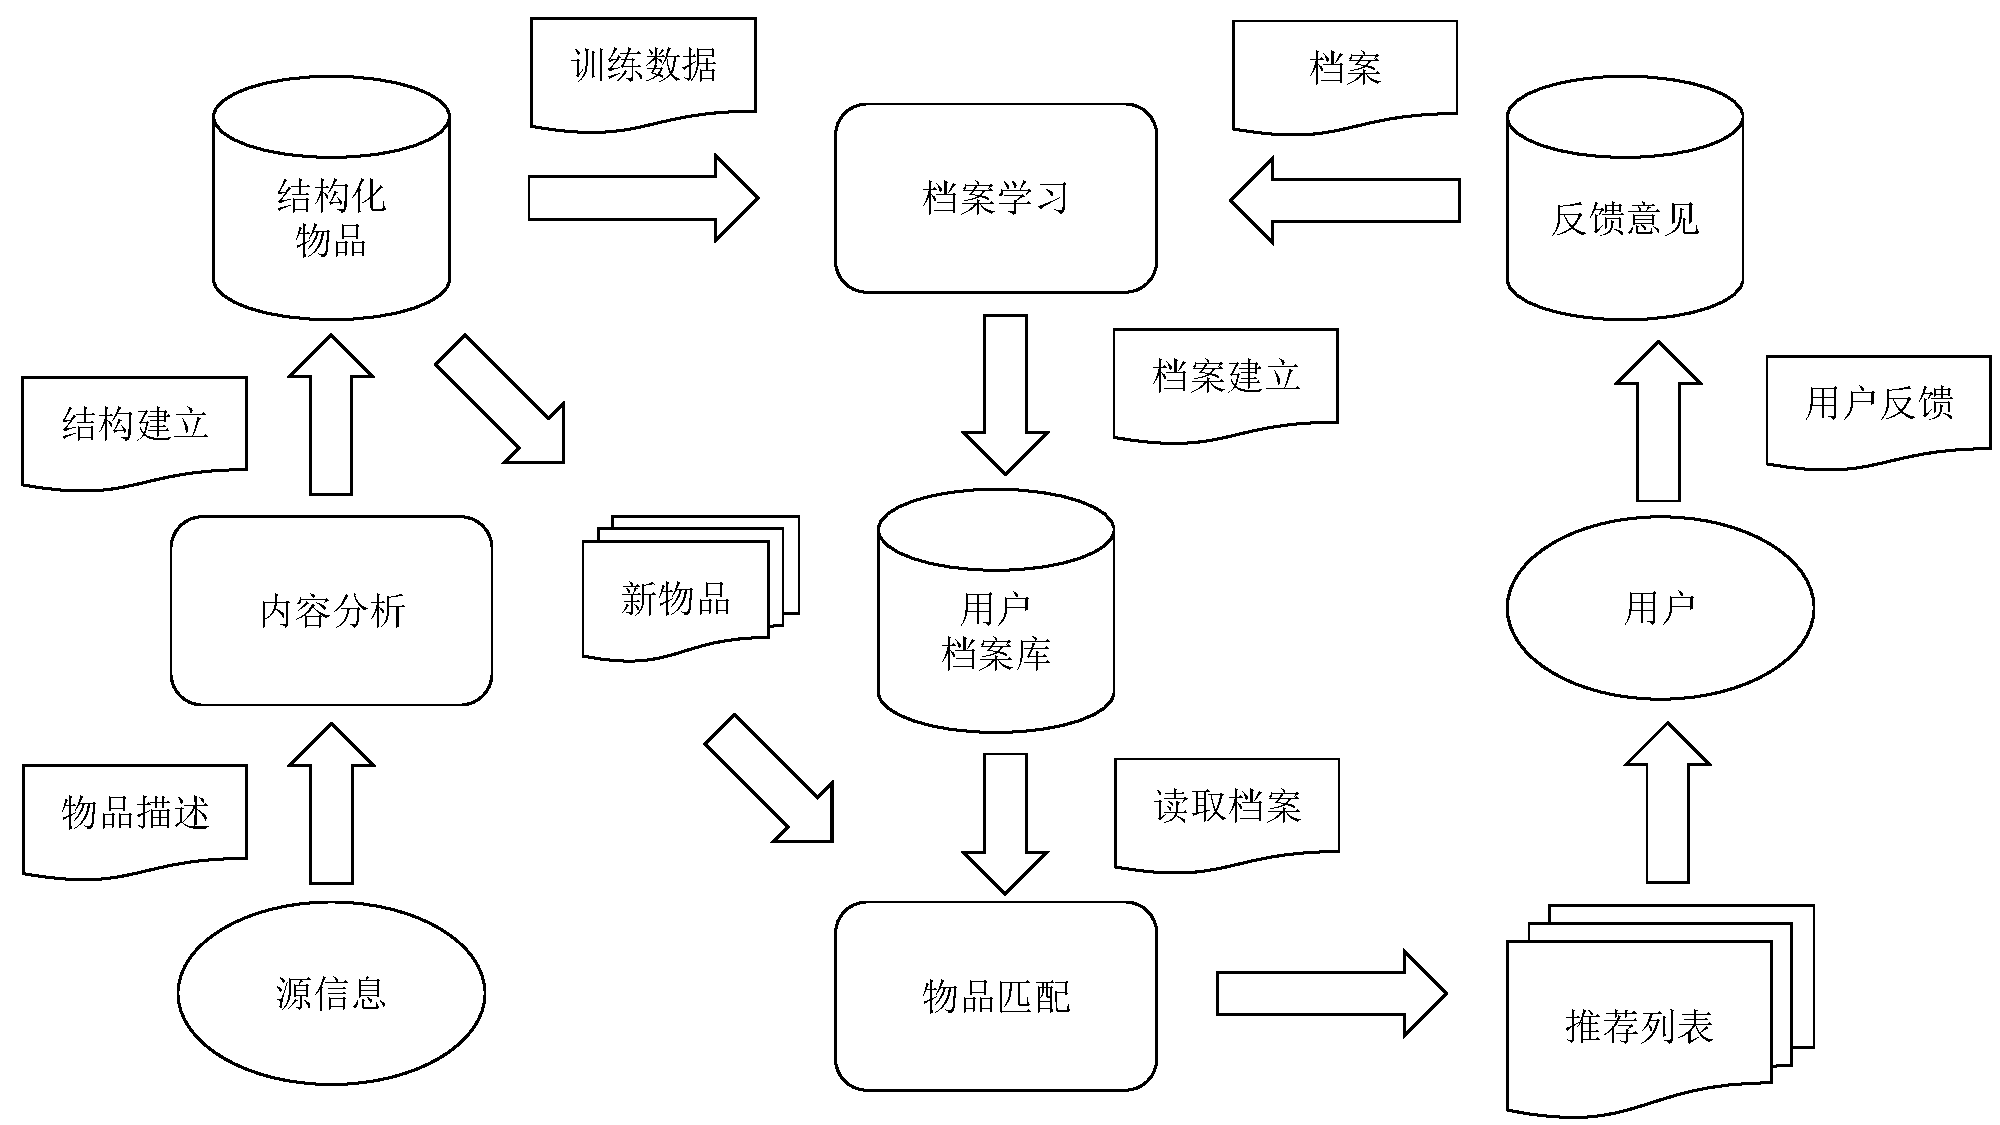
\includegraphics[width=0.75\linewidth]{02/1_cbr_arch.pdf}
 \bicaption[fig:cbr_arch]{推荐架构}{基于内容推荐算法的系统架构}{Fig}{Architecture of Content-based Recommender System}
\end{figure}

图\ref{fig:cbr_arch}展示了基于内容推荐算法的系统架构。其中椭圆形模块代表源数据,包括物品、用户信息;圆角矩形代表关键组件;圆柱形模块代表处理后的数据;箭头方向代表流程及数据流向。

在内容分析组件中,通常会借用信息检索系统中的技术,为源信息中的物品提取特征,生成物品描述以及物品的结构化内容,并将其进行存储。为了在偏好学习阶段对用户偏好模型进行创建及更新,需要存储用户对物品的评价。偏好学习组件基于用户的训练数据集,通常使用有监督学习算法建立用户偏好模型,并将该模型存储在模型仓库中。对于每一个结构化的物品,物品过滤组件会预测用户是否对该物品有偏好,将用户最可能偏好的$K$个物品生成一份推荐列表展示给用户。此外,用户的偏好可能会随时间改变,因此,系统还需维护用户的实时信息,如用户对推荐列表中物品的评价等。根据新生成的训练集,使用偏好学习组件对用户偏好进行自动更新。

\subsection{基于内容推荐系统的优点及缺点}

基于内容推荐系统的优点如下:

\begin{itemize}
 \item 用户独立性。基于内容推荐算法仅依据用户自己的评分记录建立其偏好模型。而基于协同过滤的方法需要其他用户的评分来为目标用户挑选出偏好最近邻的用户,也只能推荐近邻用户偏好的物品。
 \item 可解释性。通过列出物品特征,为用户对推荐物品做出解释。这些特征也可以作为衡量推荐系统准确性的标准,便于对内容分析策略进行调整。而在基于协同过滤的推荐算法中,唯一可以为用户进行解释就是另一个与目标用户偏好相似的用户也喜欢这个物品,缺乏可信度。
 \item 适用于物品冷启动。如果一项物品新加入到系统中,还没有被用户评分。基于协同过滤的推荐系统无法对此物品进行推荐。而基于内容的推荐系统可以克服物品冷启动问题。
\end{itemize}

同时,基于内容的推荐系统也有以下缺点:

\begin{itemize}
	\item 内容分析的局限性。基于内容推荐算法中的内容分析模块往往只能提取部分数量与类型的内容特征,这些特征是为用户建立偏好模型和进行物品推荐的主要依据。内容分析无法捕捉一些可能影响到用户购买决策的隐藏特征以及特征之间的关联。并且内容分析过程往往是领域相关的,通常需要丰富的专业领域知识。
	\item 过度匹配。基于内容推荐系统完全按照物品与用户偏好模型的匹配程度为物品进行打分、排序;并将排位较高的物品推荐给用户。因此,用户只能获取与其历史物品相似的推荐。推荐系统失去了新颖度。
	\item 用户冷启动问题。为了能够充分理解用户的偏好,建立有信服度的偏好模型。用户需要为一定数量的物品做出评价。因此,对于评价较少的新用户,系统难以给出可靠的推荐。
\end{itemize}

在机票推荐算法研究中,我们会在基于内容推荐的基础上,对物品内容分析及用户冷启动问题做出深入研究,以提升个性化机票推荐的效果。


\section{协同过滤推荐系统}

协同过滤推荐系统(Collaborative Filtering, CF)根据其他用户对物品的评价,为目标用户提供推荐。协同过滤的思想最早是在文档检索领域诞生的\cite{schafer2007collaborative},随着信息技术和互联网的发展,越来越多的诸如讨论帖、邮件清单等包含非正式内容的文档被收集到文档库中,用户难以快速了解文档的主题以及文档的质量水准,为文档检索带来了新的挑战。在二十世纪九十年代的研究发现,结合人工评价的半自动文档检索系统可以有效地解决该类问题。随后,结合人工干预的信息检索及推荐系统被大量研究\cite{goldberg1992using}。

协同过滤推荐系统的主要功能包括两个方面。第一是物品评价预测,其含义是对于一项用户未曾接触过的物品,预测用户对该物品的评价(喜好程度)。如果该物品新加入系统,缺乏用户行为记录,对其进行评价预测是较为困难的。第二是物品推荐,按照用户对物品的偏好程度,为其推荐一组物品。物品推荐通常建立在物品评价预测的基础上,除了以用户评价对物品进行排序之外,如何向用户展示推荐结果也是重要的考虑因素。近年来,协同过滤推荐领域有较多的研究成果,并且研究重心也从如何准确捕捉用户偏好转移到如何提升推荐算法的性能方面。本节我们主要介绍最常用的基于最近邻的协同过滤推荐算法。


\subsection{基于最近邻的推荐算法}
基于最近邻的推荐算法是协同过滤中最常用的方法之一,包括基于用户的最近邻算法和基于物品的最近邻算法两类。

基于用户的最近邻算法为目标用户根据相似的其他用户做出评价预测及物品推荐。首先需要建立用户间相似度的衡量方法。
\begin{equation}
\label{eq:user_sim}
	w(a,b) = \frac{\sum_j(v_{a,j}-\bar{v}_a)(v_{b,j}-\bar{v}_b)}{\sqrt{\sum_j(v_{a,j}-\bar{v}_a)^2\sum_j(v_{b,j}-\bar{v}_b)^2}}
\end{equation}

式\ref{eq:user_sim}衡量了用户之间的相似度。式中,$v_{a,j}$代表用户$a$对物品$j$的评分,$\bar{v}_a$代表用户$a$评价过的所有物品的平均评分。$j$代表用户$a$和用户$i$共同有过评分记录的物品。相似度$w(a,b)$的取值范围在$-1$到$1$之间。如果用户之间的相似度为负数,代表这两位用户之间的差异较大,在为用户挑选最近邻用户时通常会舍弃这部分用户。

\begin{equation}
\label{eq:rate_pred_ub}
	p_{a,i} = \bar{v}_a + \frac{\sum_{n \in neighbor(a)}w(a,n)(r_{ni} - \bar{r}_n)}{\sum_{n \in neighbor(a)}w(a,n)}
\end{equation}

式\ref{eq:rate_pred_ub}计算了评价预测的结果。第一项$\bar{v}_a$是目标用户的历史平均评分,第二项根据每位近邻用户的相似度以及这些用户的平均评分,对物品$i$进行评价。有些用户习惯为物品打高分,而有些用户习惯为物品打低分,公式使去中心化的方式适应用户的不同评价标准。

基于物品的最近邻算法根据用户记录中的相似物品,为用户进行评价预测及物品推荐\cite{sarwar2001item},可以认为基于物品的最近邻算法是基于用户的最近邻算法的转置。
\begin{equation}
\label{eq:item_sim}
	w(i,j) = \frac{\sum_u(v_{u,i}-\bar{v}_u)(v_{u,j}-\bar{v}_u)}{\sqrt{\sum_u(v_{u,i}-\bar{v}_u)^2\sum_u(v_{u,j}-\bar{v}_u)^2}}
\end{equation}

\begin{equation}
\label{eq:rate_pred_ib}
	p_{a,i} = \frac{\sum_{j \in relaitem(a)}w(i,j)r_{ai}}{\sum_{j \in relaitem(a)}w(i,j)}
\end{equation}

式\ref{eq:item_sim}和\ref{eq:rate_pred_ib}分别描述了物品间相似度和根据物品相似度为用户进行评价预测的方法。为了衡量物品$i$和$j$的相似度,需要使用对这两项物品都有过评价记录的所有用户评分,公式中同样进行了去中心化处理。

在最近邻推荐算法中,用户评价数据通常较稀疏。如果用户间共同评分记录的物品很少,或物品间有过共同评分记录的用户数量很少,他们容易得到很高的相似度,但这种相似度并不可靠。在系统实践中,通常仅考虑最近邻的$K$个用户或物品,并且增加一项评价记录数量的激励因子。
此外,对于流行度较高的物品,大多数用户对它的评价都很高,这类物品不具备很强的参考价值。一些协同过滤推荐算法\cite{breese1998empirical}对物品的流行度增加了惩罚项。

在系统性能方面,算法的时间复杂度与用户、物品、评价数量呈线性关系,因此需要对算法性能做进一步优化。通常系统不会维护全部用户对或物品对间的相似性,而在维持前$K$个相似项的基础上进行增量更新\cite{herlocker1999algorithmic}。此外,还可以对用户和物品进行聚类,快速定位与目标项相似的集合。

一些算法通过为物品降维的方式减少应用的复杂性,降维后的维度通常能够代表物品包含的主题特征,根据主题特征可以为用户的评价和他们潜在的偏好建立映射关系,进而根据用户的潜在偏好为其进行推荐。通过这种方法,物品评价预测往往可以在常数时间内完成。然而,这些方法在离线计算部分的时间复杂度很高,算法实现复杂,维护的成本也很高。常用的降维方法包括支持向量分解、主成分分析、特征提取等。

\subsection{协同过滤推荐的适用场景}

为了使协同过滤具备较好的推荐效果,本节对系统应具备的一些特性进行阐述,再结合本文的研究工作, 对协同过滤在机票推荐领域的应用进行分析。首先考虑数据的组织及形式,即数据分布特性:

\begin{enumerate}
  \item 系统包含一定数量的物品。如果系统中的物品较少,用户就可以自行了解每个物品,推荐系统的意义并不大。
  \item 每项物品具有一定数量的评价。如果物品收到的评价较少,则难以为用户提供可靠的预测与推荐。
  \item 用户评价条数远多于物品数量。根据协同过滤算法的原理,为了保障推荐效果,通常需要远多于物品数量的用户评价。通常,用户评价在物品中呈长尾分布,少量的热门物品拥有较多的评价,而大多数物品的评价数量较少。
  \item 物品持续性。在协同过滤系统中,用户需要分享他们曾经产生过评价的物品。在诸如新闻推荐等领域,物品的新鲜度往往只能持续数天。如果仅按照物品评价预测的结果对用户进行推荐,难以产生良好的推荐结果。
  \item 用户偏好持续性。协同过滤推荐在用户偏好不经常发生改变的领域具有较好的效果。否则,用户过去对物品的评价就不具备较高的参考价值。
\end{enumerate}

其次,协同过滤算法对系统还有一些潜在要求:

\begin{enumerate}
	\item 用户团体中存在偏好相似的用户。在团体中,与目标用户偏好相似的用户数量越多,协同过滤推荐的效果越好。反之,则难以产生预测与推荐。
	\item 物品的评价反映用户偏好。如果系统具备对物品评价的客观标准,协同过滤算法并不适用。然而,如果对物品的评价具有过强的主观性,或者具有多维度的评价标准,推荐系统需要对其进行整合与统一。
	\item 物品是同质的。系统中的物品应具备相同的本质特征,仅在用户的主观评价方面有所不同。协同过滤算法难以在不同质的物品间做出推荐。
\end{enumerate}

在机票推荐场景中,候选机票的数量很多,并且机票满足同质性。此外,用户的偏好具有较强的持久性。然而,在该领域直接应用协同过滤算法仍具有一定的挑战。首先,由于机票数量受限于航班的舱位,并且在起飞日期之前,机票的价格会产生较大幅度的持续波动,因此机票物品不具备较强的持久性。其次,用户对机票的评价较少且仅包含隐式正反馈评价,为协同过滤在机票推荐领域的应用带来了困难。

在本文的研究中,我们不直接向用户推荐机票,而是借鉴协同过滤的思路衡量航线及用户间的相似度,将协同过滤与基于内容的推荐结合起来,在冷启动场景下进一步提升机票推荐效果。

\section{主题模型}

随着网络上的信息以及专业文献库越来越丰富,自动从文本中抽取有效信息的技术变得更加重要。这类模型在文档标注、自动问答、自动生成摘要等应用场景起到很大作用。在信息检索、自然语言处理、机器学习等研究领域都对该类模型进行了深入研究。在起初几年,有监督的文档自动分类方法得到了很多的关注\cite{yang1999evaluation}。然而在很多情景下,文档库中的文档数量十分巨大,既没有预先定义的类别标签库,多数文档也没有标注类别标签。在诸如计算机、生物学等许多研究领域,文档的标签随着研究的进展发生很频繁的变化,对每篇文档进行人工标注也是不现实的。因而,基于无监督的文档模型具有更广阔的应用场景。

在研究实践中发现,基于生成模型\cite{zhong2005generative,hofmann1999probabilistic,blei2003latent,minka2002expectation}的统计方法对解决这类问题很有帮助。这类模型统称为主题模型。主题模型使用无监督策略从文档库中为每篇文档抽取可解释的表示模型。该模型将每篇文档表示成主题的混合分布,每个主题包括一组共同出现频率较高的词。主题可以将具有相似含义的词语联系到一起,还能为包含多种含义的词语确定在使用情境下的具体意义。在先前的研究中,最常见的文档表示方法是词袋模型(bag of words)\cite{zhang2010understanding}。这种模型将高维度的词汇向量转换到低维空间。综上,相比于其他的文档模型,主题模型有三点优势。第一,主题提取的过程是非监督的,即文档不需要标签以及初始化的步骤;第二,提取出的主题是可解释的,用户可以理解主题包含了哪些词汇;第三,每篇文档可以表示成多个主题的集合,可以捕捉主题之间的关系。


\subsection{主题模型概述}

主题模型的种类有很多。常见的方法包括潜在语义分析模型(LSA)、概率潜在语义分析模型(PLSA)以及潜在狄利克雷分布模型(LDA)等。

\subsubsection{LSA模型}
LSA\cite{deerwester1990indexing}的目的是为文档提取词汇的多重含义,并通过内容分析计算词汇以及文档之间的相似度。模型将文档库表示成一个矩阵,矩阵的每行代表一个词汇,每列代表一篇文档。矩阵的每个元素代表该词汇出现在文档中的频次。矩阵元素的值需要进行加权处理,考虑因素包括该词汇在文档中的重要程度以及该词汇在领域中总体信息丰富程度等。随后,对矩阵进行奇异值分解(singular value decomposition, SVD)\cite{higham2015singular}:
\begin{equation}
	A = U\sum V^T
\end{equation}

原矩阵$A$的维度是$M \times N$,分别是文档库中文档的数量以及词库的数量。矩阵$U$的维度是$M \times K$,矩阵$\sum$的维度是$K \times K$,矩阵$V^T$的维度是$K \times N$。其中$\sum$是一个对角矩阵,对角线的值由矩阵$A$的特征值组成。一般情况下,不需要使用矩阵所有的特征值,只需最大的前$K$个值就可以有效覆盖原矩阵的信息。矩阵$U$中的每列代表一个语义,每行代表一篇文档。每个元素代表该文档与该语义的相关程度;矩阵$V$中的每列代表一个关键词,每行代表一个词汇。每个元素代表该词汇与该关键词的相关程度;而中间的矩阵$\sum$的元素则表示语义和关键词之间的相关性。LSA将原本的文档特征进行降维,减轻了词汇和语义之间的复杂对应关系。

\subsubsection{PLSA模型}
PLSA是Hofmann\cite{hofmann1999probabilistic}在1999年提出了模型。该模型属于基于统计的潜在类别模型,使用了基于概率的生成模型对LSA进行改进。该模型的主要目标是区分词汇在不同语境上下文中的不同含义,主要包括两个方面,首先针对一词多义的情况下进行词义消歧;然后根据对在相同上下文中出现的单词进行聚类以揭示主题的概念。PLSA模型在诸如计算机视觉、推荐系统等领域中得到应用。

PLSA包含$K$个语义层面的隐式变量,我们称之为主题。则模型的变量包含三类。分别是文档集合$d \in D = \{d_1, \dots, d_n\}$;词汇集合$w \in W = \{w_1, \dots, w_m\}$;主题集合$z \in Z = \{z_1, \dots, z_k\}$。其中,文档和词汇是已知变量,主题是未知变量,$K$代表主题的数量,通常由先验决定。

\begin{figure}
 \centering
 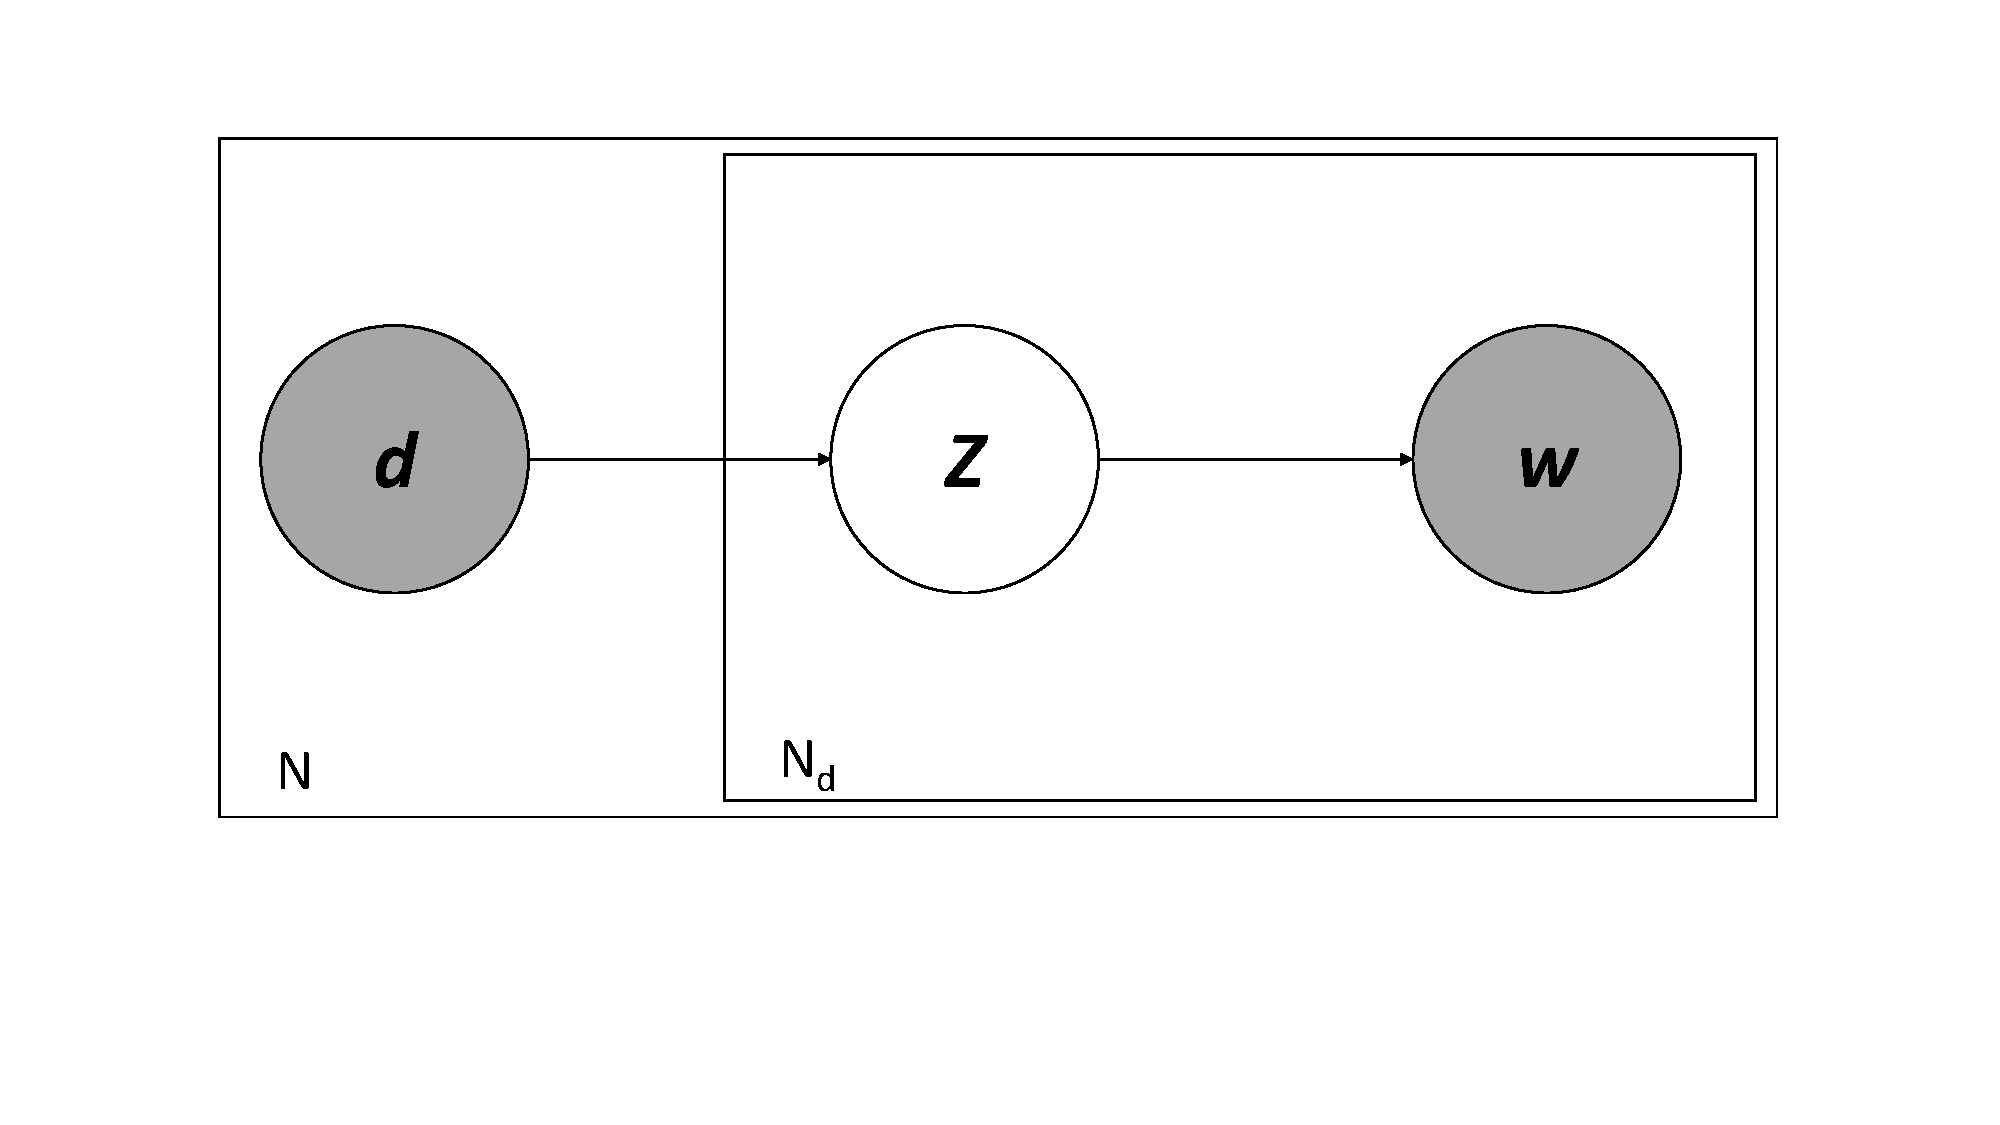
\includegraphics[width=0.7\linewidth]{02/2_plsa.pdf}
 \bicaption[fig:plsa]{PLSA}{PLSA概率图}{Fig}{Probability Graph for PLSA}
\end{figure}

图\ref{fig:plsa}是PLSA主题模型的概率图。$N$代指文档的数量,$N_w$代指每篇文档的词汇数量。带阴影的变量$d$,$w$分别代指文档与词汇,$z$代指隐式变量主题。每篇文档的生成过程描述如下:

\begin{enumerate}
\item 选择一篇文档 $d_n \sim P(d)$
\item 对于$d_n$中的每一个词汇
       \begin{enumerate}[fullwidth,itemindent=1em,label=(\alph*)]
       \item 基于多项式分布从文档中抽取主题,$z_i \sim P(z|d_n)$
       \item 基于多项式分布从主题中抽取词汇,$w_i \sim P(w|z_i)$
       \end{enumerate}
\end{enumerate}

一般情况下,我们可以认为对于给定的主题,词汇和文档是条件独立的,即$P(w|d,z) = P(w|z)$。则我们可以得到等式:
\begin{equation}
	P(w|d) = \sum_{z\in Z}P(w|z)P(z|d)
\end{equation}
\begin{equation}
	P(w,d) = \sum_{z\in Z}P(z)P(d|z)P(w|z)
\end{equation}

PLSA也可以应用在推荐系统中,将每位用户的历史购买记录视为一篇文档,购买过的没见物品视为一个词汇。可以根据模型分析出每篇文档与主题的关联。这里每个主题代表一种偏好习惯,根据每位用户的$P(z_k|d_i)$分布向量衡量用户相似度,就可以使用基于协同过滤的推荐算法。

\subsubsection{LDA模型}

在PLSA模型中,$P(z|d)$和$P(w|z)$都属于多项式分布,可以使用EM算法进行参数推导。但PLSA也有不足之处,首先参数$P(d)$是未知的,无法准确为一篇新文档设置概率值;其次,$P(z|d)$参数的数量随着文档的数量呈线性增长,可能会造成过拟合问题。

在LDA\cite{blei2003latent}模型中,同样有文档-主题分布矩阵$\Theta$和主题-词汇分布矩阵$\Phi$两个待估参数,这两个参数是分别服从超参数为$\alpha$和$\beta$的狄利克雷先验分布的随机变量。LDA与PLSA的不同之处在于:PLSA中,两个参数$P(z|d)$和P(w|z)是固定的未知变量。计算这两个变量的过程是先按照文档-主题和主题-词汇概率分布生成文档,再使用极大似然估计算法(如EM算法)对两个参数进行估计。但LDA模型将文档-主题和主题-词汇的概率分布视作服从狄利克雷先验分布的变量,而不是固定的值。通过这样设定参数,可以使用与狄利克雷分布共轭的多项式分布进行参数推导,并且还可以克服过拟合问题,比PLSA具有更好的效果。

\begin{figure}[!h]
 \centering
 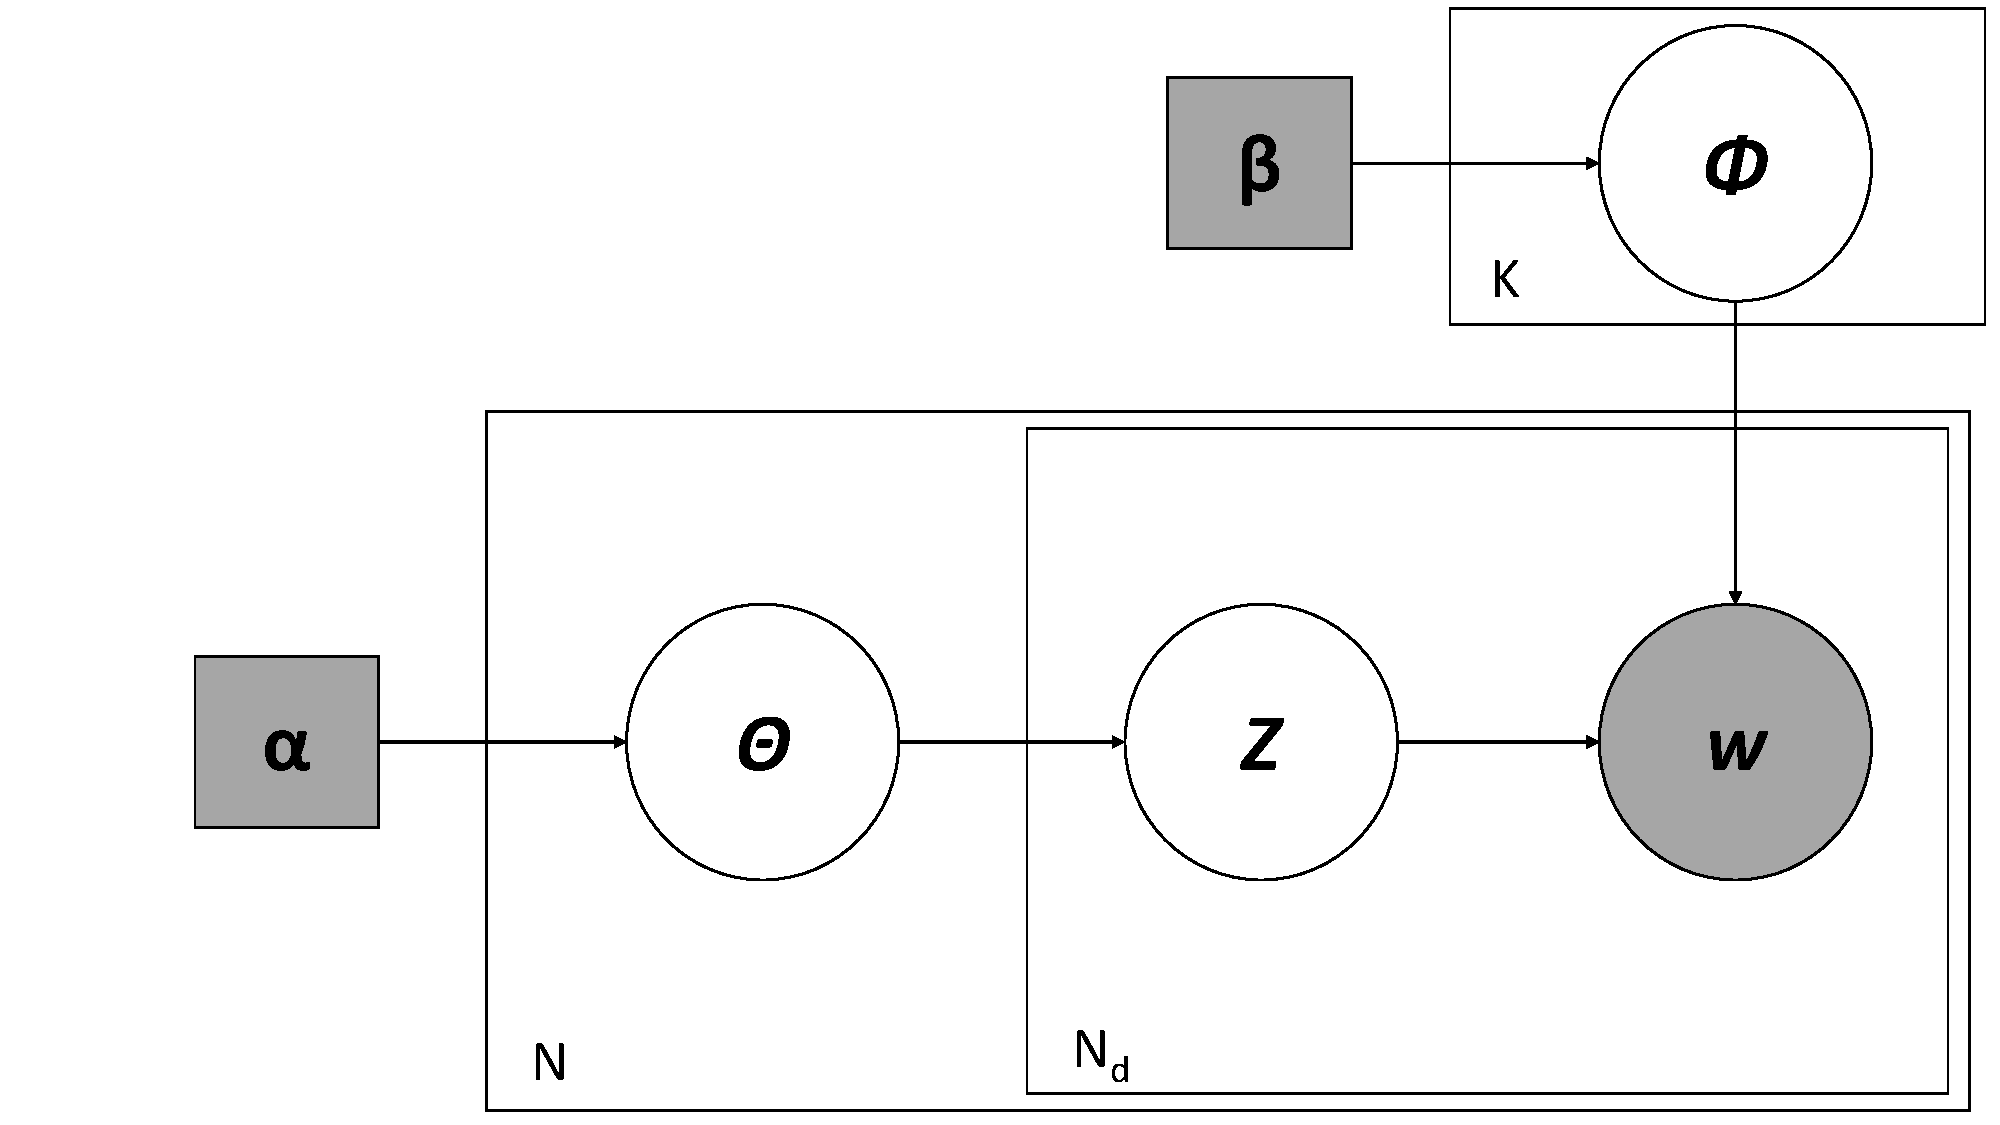
\includegraphics[width=0.7\linewidth]{02/3_lda.pdf}
 \bicaption[fig:lda]{LDA}{LDA概率图}{Fig}{Probability Graph for LDA}
\end{figure}

图\ref{fig:lda}是LDA主题模型的概率图。$N$代指文档的数量,$N_w$代指每篇文档的词汇数量,$K$代表主题的数量。带阴影的变量$\alpha$,$\beta$分别是两个待估参数的超参数,$w$代表词汇。每篇文档的生成过程描述如下:

\begin{enumerate}
\item 对每篇文档$d$,以狄利克雷先验初始化 $\theta_d \sim Dir(\alpha)$
\item 对每个主题$z$,以狄利克雷先验初始化 $\phi_z \sim Dir(\beta)$
\item 对于$d_n$中的每一个词汇
       \begin{enumerate}[fullwidth,itemindent=1em,label=(\alph*)]
       \item 基于多项式分布从文档中抽取主题,$z_i \sim Multi(\theta_{d_n})$
       \item 基于多项式分布从主题中抽取词汇,$w_i \sim Multi(\phi_{z_i})$
       \end{enumerate}
\end{enumerate}

LDA模型的参数具有超参数先验,如果先验足够准确,可以提升参数估计的准确率。并且适用于词汇数量较少的文档训练。此外,具有先验的参数可以对超参数进行调整,以适应不同的应用场景。在我们的研究中,使用主题模型来挖掘乘客和机票特征之间的关系,在共享账户情景中可以预测出乘客分布概率,以提升机票推荐的效果。


\iffalse
\section{模型参数估计}

在统计学中,参数估计\cite{heinrich2008parameter}代表使用样本数据来估计总体数据概率分布的过程。在机器学习模型中,参数往往用于描述模型的状态。而模型的真实分布是未知的,需要根据已知自变量和因变量之间的关系对整体模型的参数进行估计。一般使用独立同分布的数据集$\mathcal{X}$来表示随机变量$X$的一组观测值。$\theta$代指$X$的参数集合,取决于随机变量服从的分布。参数估计包括两个方面,第一类问题是估计参数$\theta$使得$\mathcal{X}$的出现概率最大;第二类问题是估计新的观测值$\tilde{x}$的概率。第一类问题是估计问题,而第二类问题是预测分类问题。

参数估计的方法有很多,本节我们主要介绍两种训练模型常用方法,分别是最大似然估计(Maximum Likelihood Estimation,MLE)\cite{johansen1990maximum}以及最大后验概率(Maximum a Posteri,MAP)\cite{gauvain1994maximum}。

\subsection{最大似然估计}

最大似然估计的目标是估计参数使其最大化似然函数。通常似然函数都有如下的形式:
\begin{equation}
\label{eq:ml}
	L(\theta|\mathcal{X}) = p(\mathcal{X}|\theta) = \bigcap_{x \in \mathcal{X}}{X=x|\theta} = \prod_{x \in \mathcal{X}}p(x|\theta)
\end{equation}

式\ref{eq:ml}是随机变量对于一组样本的似然函数,其中$L(\theta|\mathcal{X})$的含义是随机变量$X$产生样本$\mathcal{X}$的概率。在参数估计过程中,我们通常对似然函数取$\log$以简化计算过程,我们可以定义新的目标函数:

\begin{equation}
	\hat{\theta}_{ML} = \arg\max_\theta \mathcal{L}(\theta|\mathcal{X}) = \arg\max_\theta \sum_{x \in \mathcal{X}}\log p(x|\theta)
\end{equation}

在最大似然估计的过程中容易出现过拟合的问题。由于待估参数过于贴合观测样本的特征,将观测数据集中的噪声也作为模型特性进行学习,因而降低了模型的泛化能力。可以使用添加正则项的方式解决过拟合问题。于是目标函数可以更新为:

\begin{equation}
	\hat{\theta}_{ML} = \arg\max_\theta \sum_{x \in \mathcal{X}}\log p(x|\theta) + \lambda\sum_{j=1}^n\theta_i^2
\end{equation}

通常我们使用梯度下降算法进行参数训练。以梯度的负方向作为迭代方向,并确定学习速率。通过参数迭代使其逐步接近目标点。根据最优化理论,若优化目标函数是非凸的,则可能只得到局部极大似然。可以采取模拟退火思想以及进行多次初始化训练的方法克服这个问题。

对于新观测值问题,由观测样本集$\mathcal{X}$得到样本$\tilde{x}$的概率可以根据已估计的参数$\hat{\theta}_{ML}$获得:

\begin{eqnarray}
p(\tilde{x}|\mathcal{X})& = &\int_{\theta \in \Theta}p(\tilde{x}|\theta)p(\theta|\mathcal{X})d\theta \nonumber \\
& \approx &\int_{\theta \in \Theta}p(\tilde{x}|\hat{\theta}_{ML})p(\theta|\mathcal{X})d\theta = p(\tilde{x}|\hat{\theta}_{ML})
\end{eqnarray}


\subsection{最大后验概率}

最大后验概率与最大似然估计很相似。相比于最大似然估计,MAP为待估参数设置了先验分布$p(\theta)$。根据观测样本使待估参数达到最大后验概率,属于贝叶斯方法。新的目标函数如下:

\begin{eqnarray}
	\hat{\theta}_{MAP} &=& \arg\max_\theta p(\theta|\mathcal{X}) \nonumber \\
	&=& \arg\max_\theta \frac{p(\mathcal{X}|\theta)p(\theta)}{p(\mathcal{X})} \nonumber \\
	&=& \arg\max_\theta {\sum_{x \in \mathcal{X}}\log p(x|\theta) + \log p(\theta)}
\end{eqnarray}

可以看出,相比于MLE的目标函数,最大后验概率的目标函数增加了一项先验分布。这项先验分布可以用来挖掘观测集额外的信息,也可以用于预防过拟合问题。在贝叶斯方法中,参数$\theta$也认为是随机变量,而不是固定的未知数值。通常使用超参数为$\theta$设置先验。参数的训练方法与MLE类似,都可以使用梯度下降法。对于新观测值的概率,同样使用已估计的参数$\hat{\theta}_{MAP}$得到。

\begin{equation}
p(\tilde{x}|\mathcal{X}) \approx \int_{\theta \in \Theta}p(\tilde{x}|\hat{\theta}_{MAP})p(\theta|\mathcal{X})d\theta = p(\tilde{x}|\hat{\theta}_{MAP})
\end{equation}
\fi

\section{本章小结}
本章介绍了与论文研究工作相关的一些技术。首先介绍了基于内容推荐系统,分析了该系统的系统架构及流程,还分析了基于内容推荐算法的优势与劣势。其次介绍了协同过滤推荐技术,介绍了基于最近邻的协同过滤推荐算法以及算法的适用场景。同时结合本文工作,分析了在机票推荐领域应用基于内容推荐和协同过滤推荐的挑战性。最后介绍了主题模型,分析了三类常用的生成模型,包括它们的参数推导、生成过程等。这三种技术为我们后续章节的研究做了理论铺垫。










%# -*- coding: utf-8-unix -*-

\chapter{机票数据分析及基线机票推荐算法}
\label{chap:baseline}
本章对研究用到的机票数据进行简要介绍及内容属性分析。在此分析的基础上,
给出用户偏好模型的表示方法并根据用户的偏好进行机票个性化推荐。
根据实验结果评估推荐算法的效果。本章的算法作为一个基线算法,是后续章节算法改进的基础与对照。

\section{数据来源及描述}
本论文研究工作使用的数据由国内知名的在线票务服务商提供。数据以表的格式组织,每条数据为一张机票订单。原始数据记录中的主要字段如表\ref{tab:fields}所示。
表格的前两项分别标识了唯一的订单以及对应的订票用户;由于国内部分城市有两个或更多个机场,所以需要标注航班的起飞机场和到达机场;舱位等级主要包括头等舱,商务舱和经济舱三个大类;飞机型号包含了飞机的大小等特征。

\begin{table}[!hpb]
  \centering
  \bicaption[tab:fields]{字段介绍}{原始机票订单数据的字段}{Table}{Fields of 
  Flight Data}
  \begin{tabular}{|c|c|} \hline 
    字段名称 & 字段描述\\ \hline
    Order Id & 订单ID \\ \hline
    User Id &  账户ID \\ \hline
    Order Date & 用户订票日期 \\ \hline
    Order Time & 用户订票时间 \\ \hline
    Takeoff Date & 航班起飞日期 \\ \hline
    Takeoff Time & 航班起飞时间 \\ \hline
    Departure City & 航班起飞城市 \\ \hline
    Arrival City & 航班落地城市 \\ \hline
    Airline & 航班所属航空公司 \\ \hline
    Departure Port & 航班起飞机场 \\ \hline
    Arrival Port & 航班到达机场 \\ \hline
    Class & 舱位等级 \\ \hline
    Price & 机票价格 \\ \hline
    Ticket Policy & 退改签政策 \\ \hline
    Craft Size & 飞机型号 \\ \hline
  \end{tabular}
\end{table}

表格中的字段表明了机票数据高度结构化的特性。机票数据的属性与书籍、电影、音乐等物品的属性不同。后者的属性通常仅作为物品分类的依据,不能直接反映物品本身的内容。而机票数据的属性则可以代表机票本身的内容,进而直接影响用户的购买决策。另外,不同于上述物品固定的静态属性,机票的价格属于动态属性,即使对于相同航班的同一等级的舱位,其票价在起飞前会发生持续变动,并且变动的幅度很大。而价格作为机票内容中相当重要的一项,会在很大程度上影响用户的选择。因此,我们不能把具有相同航班号和舱位等级但价格不同的机票当作同一个物品;
也难以直接使用以 User-Item 矩阵表示的协同过滤类型的方法进行机票推荐。根据机票数据具备的上述特性,我们主要使用基于内容的方法进行机票推荐。
此外,用户搜索时产出的候选机票数量约为一百左右,远低于传统推荐系统中成千上万的物品数量,但是每项候选机票都算作一个新的物品。机票个性化推荐相当于将这数百项候选机票按照用户的偏好进行个性化排序,并按照排序后的结果向用户展示。因此,我们首先需要为每位用户建立偏好模型。

\section{用户偏好模型构建}

用户在决策购买机票时,可能会受很多因素的影响。有些用户属于价格敏感类型,倾向于选择价格较低的机票;有些用户可能因公出差,而公司和某些航空公司有合作关系,航空公司就是这类用户的首要考虑因素;起飞时间、出发机场等属性则是和用户的个人行程安排相关。在构建用户偏好模型时,我们着重关注直接反应机票内容的特征属性。

\subsection{机票数据预处理与特征选取}

从表\ref{tab:fields}中可以发现,机票的特征主要分为两种类型。一种是包括机票价格、起飞时间的连续型特征,而其余的均为离散型特征。为了便于构建模型,我们将两个连续特征进行离散化。起飞时间的离散化过程比较直观,可以将时间分为上午、下午、傍晚、夜间等几个区间。而价格特征的离散化较为复杂。首先,不同航线具有不同的基准价格;其次,对于同一条航线,在距离起飞日期不同的天数,同一个价格可能代表不同的价位相对高低程度。结合实际的推荐应用场景,我们使用了如下公式作为价格指数:\\
\begin{equation}
	P_{KPI} = \frac{P_{std} - P_{cur}}{P_{std} - P_{low}}
\end{equation}
其中,$P_{std}$是该航班的经济舱全价,是航空公司给出的标准价格,变动频率很小(通常以年为单位);$P_{cur}$是当前机票的价格,在每条订单记录中可以获取。$P_{low}$是本次搜索页面中的最低价格。
从几项参数的含义可以看出,如果用户选择的机票价格很低,分子越大,等式的值越接近1;反之,等式的值越小,当用户选择的票价高于经济舱全价时,价格指数的值小于0。因此,价格指数越大,代表用户对票价越敏感;反之亦然。我们可以使用价格指数代表多变而重要的价格特征。并且,通过该公式计算出的价格指数与航线、距离起飞日期天数等因素无关,进而具有良好的通用性。得到价格指数后,可以结合业务领域知识将其划分为数个有代表性的区间\par
完成对连续型特征的离散化后,我们又选取了起飞机场、到达机场(对于包含多机场城市的航线)、航空公司、舱位等级、退改签政策、飞机型号等关键特征。这些特征可以初步理解为对机票内容的概括。至此,机票的一个特征都可以表示为一个向量,该向量的每个维度代表该特征对应的每个可行的取值(区间);每张机票也可以表示为一个向量,该向量的每个维度表示机票在每个特征的取值。用户在一个特征上的偏好可以由用户在每个取值所占的选择频数百分比来描述,选择频数可以通过用户的历史订单统计。\\
\begin{equation}
\label{eq:dict}
	\mathbf{p_f} = [alternative:frequency,\dots]
\end{equation}
\begin{equation}
\label{eq:pref}
	\mathbf{P_u} = [\mathbf{p_0},\mathbf{p_1},\dots,\mathbf{p_{|f|}}]^T
\end{equation}\par
式\ref{eq:dict}描述了用户在一个特征上的偏好。$\mathbf{p_f}$中的每个键值对代表了特征可能的取值及该用户选择的频数百分比。
式\ref{eq:pref}描述了用户的机票偏好模型。机票共有$|f|$个特征。$\mathbf{P_u}$中的每个向量代表了用户在机票各个特征的偏好情况。
考虑到不同的用户可能侧重于不同的特征,在得到机票的主要特征和用户的偏好表示模型后,
还需要为每个特征赋予权重。

\subsection{机票特征权重的计算}

特征的权重代表了该特征对用户的重要程度。通常,在用户更侧重的特征上,用户的偏好会更加集中。我们使用信息熵todo:cite来描述用户偏好的集中程度。信息熵的公式如下:
\begin{equation}
\label{eq:entropy}
	H(\mathbf{X}) = E[-ln(P(X))] = - \sum_{i=1}^n P(x_i)lnP(X_i)
\end{equation}\par


\section{基于用户偏好的机票个性化推荐算法}

\section{实验结果分析}

%# -*- coding: utf-8-unix -*-

\chapter{机票推荐中的冷启动问题}
\label{chap:cold}

冷启动问题一般分为物品冷启动和用户冷启动。前者的含义是当一件物品新添加到物品库中,在还没有用户使用过的情况下如何将其推荐给用户;后者的含义是当一名新用户来到推荐系统,在完全没有用户偏好的情况下如何为用户推荐适当的物品。冷启动问题是推荐系统需要面对的严峻问题。如果处理不好冷启动问题,系统内添加的新物品可能永远都无法向用户推荐;也会影响到新用户的体验,造成用户流失。

在机票推荐系统中,由于机票的数量非常有限并且每条航线上的航班较为固定,通常不会面临物品冷启动问题。而机票本身属于低频、刚需物品。因此机票推荐系统面临的主要问题是用户冷启动问题。在传统的推荐系统中,有一些办法可以解决用户冷启动问题:如在电子商务、书籍网站,用户往往会先提供物品的类别、品牌等信息,随后可以将类别下购买人数的商品推荐给新用户;而在视频、新闻等内容网站,可以在新用户注册时让用户勾选一些感兴趣的主题,即使没有有效获取用户的偏好主题,仍可以将总体最热门的、最实时的内容呈现给用户。

在机票推荐研究领域,由于其业务的特殊性,这两种做法均有不足之处。由于机票具有动态属性,难以静态地描述;并且每个航班的机票数量最多在一两百左右,造成的结果是热门物品与冷门物品之间的差别很小。因此很难单纯以热门程度进行推荐。在第三章,图\ref{fig:res_pref_rec}中的结果表明,以航班热门程度排序的策略难以表现出好的推荐效果。其次,影响用户购买决策的因素有很多,用户每次选购机票时注重的属性可能会因为用户的日程安排、出行目的的不同而发生变动。而在内容网站,用户的兴趣主题一般不会发生频繁变动。

在第三章中,图\ref{fig:user_user_percent}的统计结果表明,在北京-上海这条热门程度很高并且订单、用户数量比最高的航线上,平均每位用户的订单数量仅为两单,仍有$60\%$的用户在过去两年仅订过一单,$90\%$的用户仅订过不多于四单。订单数量在四单及以下的用户占了订单总数的$60\%$。在机票票务服务业务领域,用户冷启动现象也严重影响到用户体验及机票推荐效果。因此需要对冷启动问题展开深入研究。


\section{航线分析及推荐差异}
本小节我们主要对机票推荐中冷启动问题对推荐结果带来的负面影响进行分析与阐述。此处我们仍然选取第三章中提到的四条热门航线进行分析。

\subsection{航线特征分布及用户行为分析}

我们在第三章中提出的机票推荐算法首先将用户数据按照航线进行分割。并为每个用户在每条他选购过机票的航线上独立维护一个偏好模型。这样的做法细化了推荐粒度,使用与目标推荐航线相同的航线来进行建模可以得到更贴合的用户偏好。但是用户的历史订单数据却分散到各个航线。如果在待推荐航线上的训练数据过少,则难以精确刻画用户的偏好。在此我们首先分析航线间的差异;并分析按航线为用户提取偏好对推荐效果带来的影响。

\begin{figure}
\centering
\subfigure[北京-上海航线价格等级分布图]{
 \label{fig:sha-pr}
 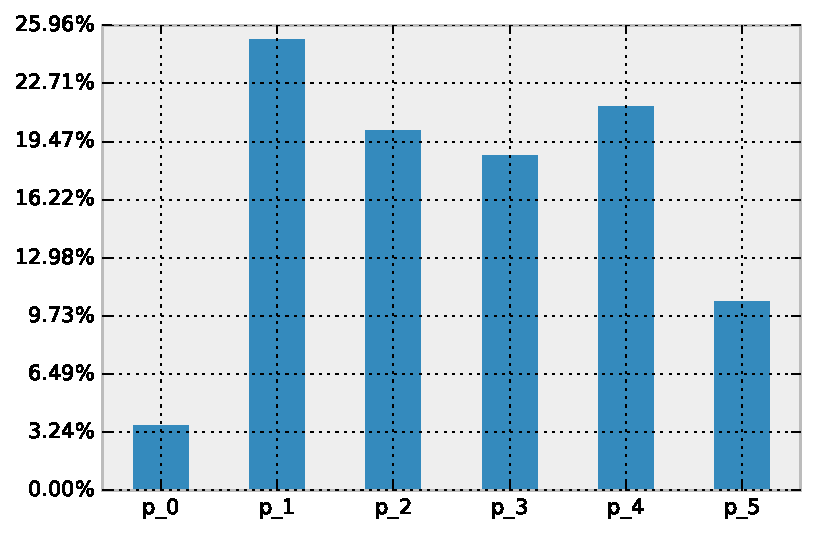
\includegraphics[width=0.49\linewidth]{06/3_pr_dis_bjs.pdf}}
\subfigure[北京-西安航线价格等级分布图]{
 \label{fig:xiy-pr}
 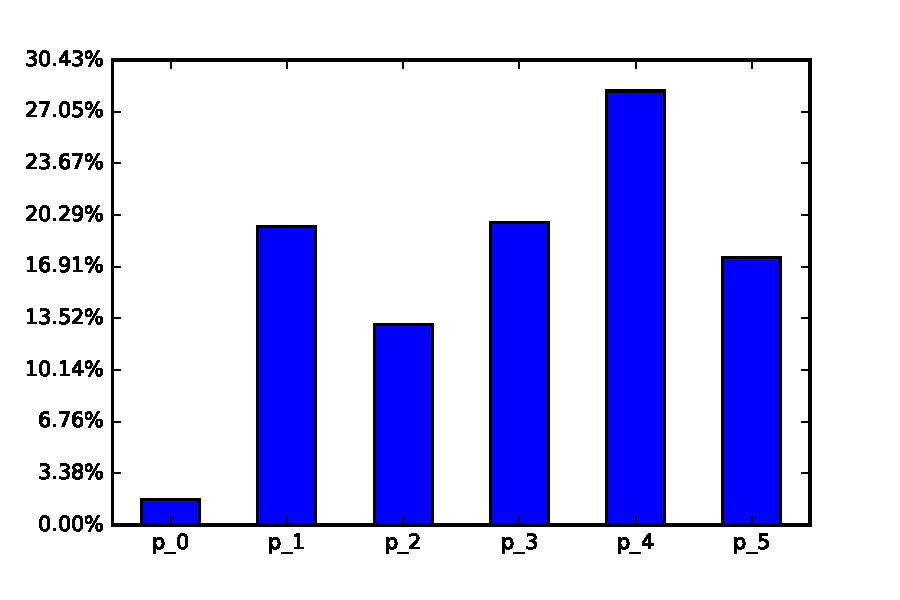
\includegraphics[width=0.49\linewidth]{06/4_pr_dis_xiy.pdf}}
\bicaption[fig:pr_dis]{价格等级分布}{航线间价格指数分布差异}{Fig}{Figure for Variety of  Price Range}
\end{figure}

图\ref{fig:sha-pr}展示了北京到上海航线上的价格指数的分布情况,其横轴的各个标签代表不同的价格指数等级,根据前文提出的价格指数概念,我们将价格指数按照增序划分到$P_0 ~ P_5$六个等级,机票订单价格逐级下降;其纵轴代表位于该价格等级的订单占订单总量的百分比;类似地,图\ref{fig:xiy-pr}展示了北京到西安航线的价格指数分布情况;两图对比可以看出,两条热门航线上价格指数等级的分布占比既有相似之处,也有部分差异。相似之处在于:价格位于最高区间的机票订单数量最少,价格位于最低区间的订单量也较少,而大部分订单集中在中间的价格区间;差异之处在于:在北京到上海航线,高价格区间的订单总体数量占比较大,
其中$P_1$区间的订单总量最多,达到$25\%$;而在北京到西安的航线,低价订单的总体占比较大,
$P_4$区间的订单总量最多。这也与我们之前结合订单、用户数量比得出的航线间出行目的差异相吻合。根据上图的分析我们可以发现,不同航线上的特征分布有所不同。

\begin{figure}
\centering
\subfigure[北京-上海航线航司标准熵分布图]{
 \label{fig:sha-h}
 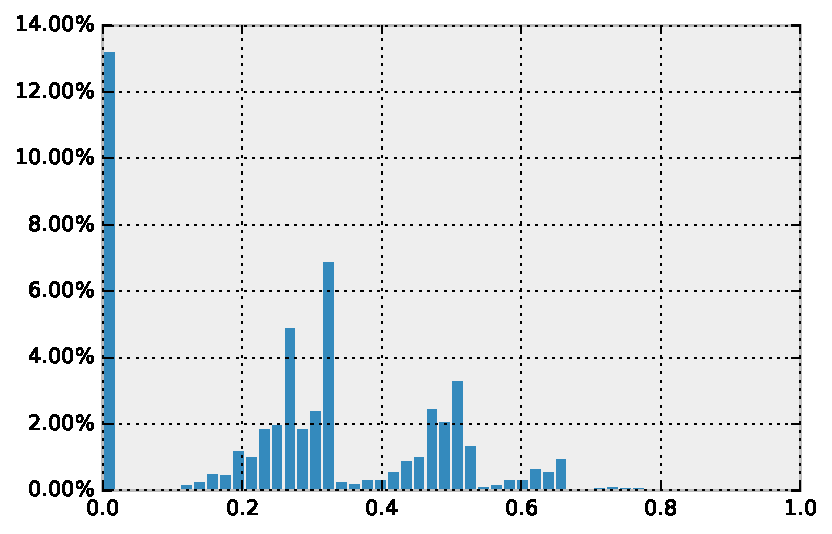
\includegraphics[width=0.49\linewidth]{06/1_entropy_airline_sha.pdf}}
\subfigure[北京-西安航线航司标准熵分布图]{
 \label{fig:xiy-h}
 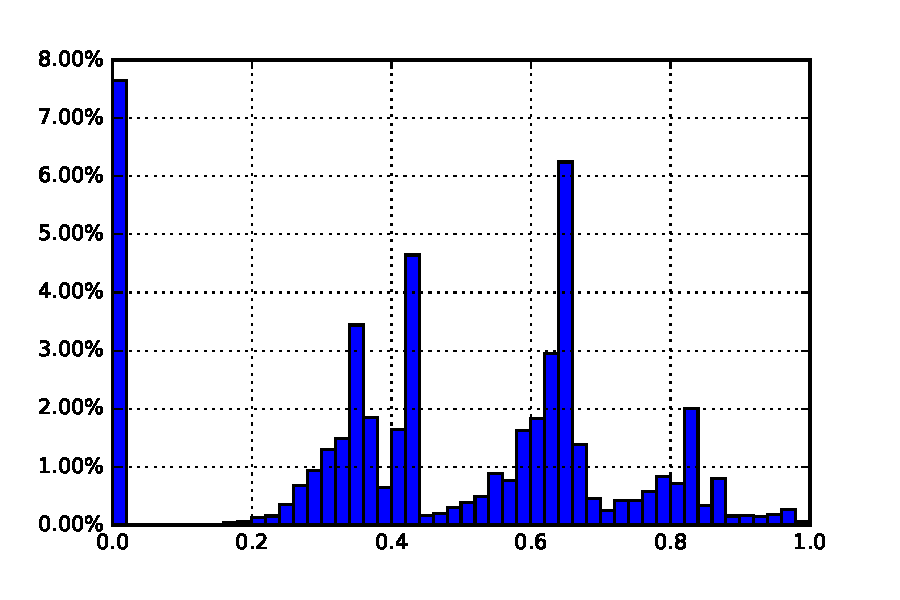
\includegraphics[width=0.49\linewidth]{06/2_entropy_airline_xiy.pdf}}
\bicaption[fig:h_dis]{标准熵分布}{航线间标准熵分布差异}{Fig}{Figure for Entropy Variety of Air Routes}
\end{figure}

图\ref{fig:sha-h}和图\ref{fig:xiy-h}分别展示了北京到上海航线和北京到西安航线的航司标准熵分布图,横轴代表标准熵值,
是将根据公式\ref{eq:entropy}计算出的熵值除以向量的维度进行归一化得到的值。其取值范围在$[0,1]$,用户的偏好集中程度随着熵值的减小而增加。纵轴代表用户的数量占比,即航司偏好的标准熵在该值的用户占用户总数的比例。两条航线都是在标准熵小于0.02的用户数量最多;北京到上海航线上,有更多比例的用户在航司维度的标准熵小于0.02,并且整体熵值偏小,证明在该航线上,用户对航司的偏好更集中。而北京到西安航线,更多的用户集中在0.6附近,相比于前者,用户在该航线上的对航司的偏好更加分散。

至此,我们根据图\ref{fig:pr_dis}反映了不同航线上总体特征分布的差异,这是航线之间客观存在的差异,可能与航空公司的定价策略及票源供给策略等挂钩。还根据图\ref{fig:h_dis}分析了不同航线上用户偏好集中程度的差异,这属于用户主观行为的差异,会受到航线的属性、起飞城市和落地城市的社会性质等因素影响。我们分析对比了客观、主观两个方面的因素对航线造成的影响,也因此造成了航线间的差异。

\subsection{航线差异对机票推荐造成的影响}

分析了航线特征分布及用户偏好集中程度的差异后,需要研究航线间差异对推荐效果的影响。我们的基本思路是使用用户在其他航线的模型为其进行机票推荐,并评估推荐效果。如果使用其他航线模型与仅使用本航线模型的推荐效果相差不多,则证明航线差异不影响机票推荐;反之则证明航线差异对推荐结果的影响不可忽视。

\begin{figure}
 \centering
 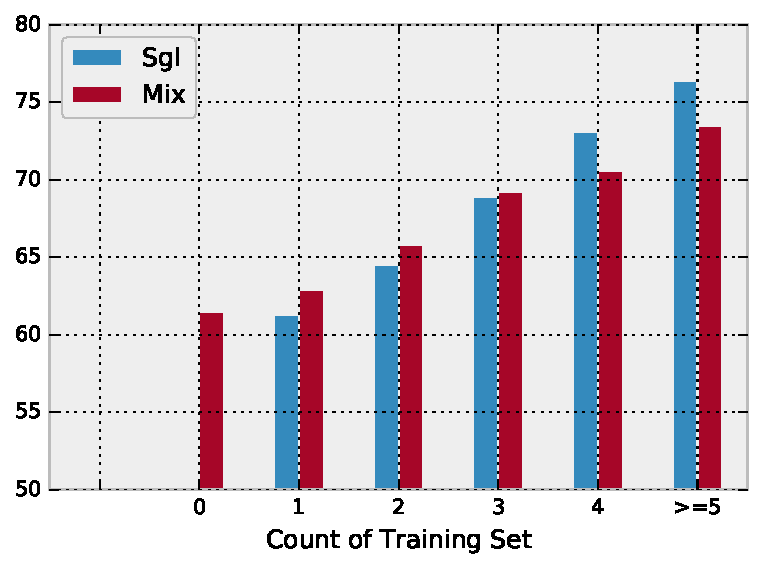
\includegraphics[width=0.75\linewidth]{06/5_res_of_sgl_all.pdf}
 \bicaption[fig:slg_all_rec]{航线推荐效果对比}{单一航线与全航线模型的推荐效果对比}{Fig}{Accuracy of Recommendation for Single and All Air Routes}
\end{figure}

图\ref{fig:slg_all_rec}展示了在北京到上海航线上分别仅使用目标航线历史订单建立用户模型(Sgl,以下称为单一航线模型)以及使用所有航线(包括目标航线)数据建立用户模型(All)进行机票推荐的效果。为了获取有效推荐结果,必须抽取出一条订单作为测试订单,我们将测试订单所在航线定义为目标航线,用户在该航线上其他订单定义为训练订单。对于单一航线模型推荐算法,我们无法为在该航线上只有一条订单的用户进行推荐结果验证。
图的横轴代表用户在目标航线的训练订单条数。纵轴代表推荐平均准确率。对于单一航线模型的推荐算法,其训练订单的数量等于横轴标注的数量;而对于全航线模型推荐算法,训练订单还要再加上用户在其他航线上的历史订单,数目不确定。但在我们要解决的问题中,用户的订单量普遍较为稀少,所以该模型中的总训练订单数量一般不会太大。

从图中我们可以看出,当目标航线训练订单数量为三条及以下时,使用全航线模型的推荐效果好于单一航线模型。两者之间的差距随着订单数量的增加而减小。当目标航线上的训练订单数达到三条时,两种模型的推荐效果没有明显差异,但单一航线模型的计算开销和I/O吞吐开销都较小。当训练订单多于四条时,使用单一航线模型的推荐效果好于全航线模型。由此我们可以得出结论,在用户建模时使用的数据不一定越多越好,由于航线差异可能导致其他航线的用户模型稀释了用户在目标航线上的偏好。为用户按照航线区分特征分布模型对于订单数量在三单以上的用户具有较好的推荐效果。

从图中还可以发现,当目标航线没有训练订单时,全航线模型的机票推荐结果也相当不错,与只有一单训练订单时的单一航线模型推荐结果相差无几。可以说明当用户的订单量较少时,学习的用户模型具有一定的偶然性。并且用户在其他航线上的偏好具备一定程度上的借鉴意义。在实际生产环境中,我们不区分测试订单、训练订单的概念,为了兼顾系统性能与用户体验,可以直接使用该用户在其他航线上的数据进行偏好建模。

\section{航线冷启动问题的分析}
前文我们分析了航线间差异及对个性化机票推荐带来的影响。本节我们针对航线冷启动问题进行研究。航线冷启动问题的含义是用户在需要进行推荐的目标航线上没有历史订单或订单数量较少。根据前文的对照实验结果,我们主要针对的用户是用于建模的目标航线训练订单数量少于三单的用户。

\subsection{航线间差异的量化}

这类用户由于订单量较少,无法在目标航线建立精确的特征分布模型,但在其他航线具有部分订单。为了针对这批用户解决航线冷启动问题,一个基础的思路是我们需要将用户在其他航线上的模型进行适当的修正,使其能够克服航线间的差异,以符合用户在目标航线上的偏好。为此,我们首先需要能够量化航线间的差异程度。

我们仍使用相似度函数来分析航线间的差异。对于结构化的物品。我们可以对其进行特征提取,则物品可以由同构的特征-取值键值对表示。在衡量物品的整体相似度时,可以先按照每个特征的内容组成衡量局部相似度,再将个局部相似度进行融合,就可以得到整体相似度。相似度融合的策略一般是以特征在整体中的相对重要程度定义一个权重指数。因此,整体相似度的衡量公式可以定义为:
\begin{equation}
\label{eq:line_sim}
	Sim(A,B) = \sum_{f \in F}w(f) \times \sigma(f)
\end{equation}

$w_f$代表特征权重。$\sigma_f$是特征局部相似度衡量方法。为机票进行相似度衡量时,机票的每一个特征对应具体数值,我们需要为每个特征所有可能的取值之间定义相似度分数,往往需要借鉴业务领域知识。在航线相似度衡量中,我们可以从与机票类似的角度出发,将航线以多维度特征表示。航线的关键特征与前文提到的特征一致,包括价格、起飞时间、机型、舱位等级、航司和退改签政策。与机票不同的是,航线上的每个特征包含所用用户订单。这里,我们使用航线在每个特征的总体分布向量来代表该航线的对应特征。此外,我们在之前的章节展示了不同航线在用户行为方面有一定的差异,表现在该特征的用户标准熵的分布有较大
差异。因此,用户行为也作为我们衡量航线相似度的一个考虑因素。

航线每个特征的分布可以表示为向量,每个向量所有维度的取值之和为1。我们对特征使用同样的离散化策略。对于航司特征,其种类多达数十种,而每条航线上出现的航司组合不尽相同,往往只有不到十种。如果将所有的航司都罗列到一个向量中,则大多数维度的分布百分比都是0,会对相似度的衡量带来干扰。因此,我们使用字典来维护这个特征。在衡量两条航线在航司的相似度时,我们首先将各自的字典进行扩容,使它们的键包含两条航线上航空公司的并集,可以将航司特征也转化为向量。这里我们使用欧几里德距离作为衡量航线在一个特征上分布差异的公式:
\begin{equation}
	Dist(\mathbf{X},\mathbf{Y}) = \sqrt{\sum_{i=1}^{|X|}(x_i-y_i)^2}
\end{equation}
\begin{equation}
\label{eq:a_sim}
	DistSim(\mathbf{X},\mathbf{Y}) = \frac{1}{Dist(\mathbf{X},\mathbf{Y})}
\end{equation}

欧氏距离衡量了两个向量在空间上的距离,适合在两个相同维度以及量纲的向量之间进行比较。在公式中,$\mathbf{X}, \mathbf{Y}$代表需要计算相似度的向量。式\ref{eq:a_sim}定义了以欧式距离为基础的相似度衡量公式,可以得出当两个向量的欧氏距离为0时,它们的相似度为$1$,且随着欧式距离的增加,向量间相似度递减。
对于用户行为相似度的衡量,结合上一节我们统计过用户熵值分布百分比,我们可以将标准熵在$[0,1]$取值区间内均匀划分为$50$个区间,将每个区间视作一个维度,
将用户熵值在一个特征上的分布也转化为向量,记作$S(f)$。
下公式给出结合航线分布和用户行为的航线间特征相似度衡量方法:
\begin{equation}
	\sigma(f) = DistSim(\mathbf{f_a,f_b}) + DistSim(S(\mathbf{f_a}),S(\mathbf{f_b}))
\end{equation}
\begin{equation}
	\overline{S}(\mathbf{f_a}) = \frac{\ln |f| - S(\mathbf{f_a})}{\ln |f|}
\end{equation}
\begin{equation}
	w(f) = \overline{S}(\mathbf{f_a}) + \overline{S}(\mathbf{f_b})
\end{equation}

$f_a, f_b$是待比较航线上的一个特征,第一项代表航线间特征分布的相似度,第二项代表在该特征上用户行为分布的相似度。每个特征的权重定义为两条航线上该特征分布的标准熵之和。计算出两条航线在所有特征的权重后,将所有值进行归一化就得到了标准权重。至此,我们从特征分布和用户行为两个方面量化了航线间的差异。在解决航线冷启动问题时,可以根据这个量化方法,对用户在非目标航线的模型进行修正,进而将其应用在机票推荐中。

\subsection{最优相似航线的选取及修正模型}
本小节主要介绍我们如何根据航线间差异量化方法为航线冷启动用户选取最优相似航线并进行模型修正。一个最简单的方法是从用户订单中选出与目标航线差异度最小的航线,将用户在该航线的特征分布模型应用在目标航线。这种做法存在几个问题。首先,用户可能在与目标航线相似度最高的航线上也属于冷启动跃用户,这条航线虽然最符合我们的策略,用户在其航线上的特征分布模型也具备相当大的偶然性,因而对提升推荐效果起不到显著作用;其次,虽然选出了与目标航线差异最小的航线,并且用户有足够多的订单,但用户在那条航线上的模型也与该航线的整体特征分布有密切联系,因而无法直接使用在目标航线的推荐中。

鉴于以上几点,我们首先需要选取合适的非目标航线,其次还要对用户在该航线的模型进行修正。为了避免第一个问题,我们在与目标航线相似度的基础上加上用户在本航线的订单数量作为一个激励因子,将航线相似度和订单数量都作为度量因素,提出了加权相似度公式:

\begin{eqnarray}
\label{eq:rsim}
	ReSim(\mathbf{R_a,R_b}) & = & \log{|O_b|} * Sim(\mathbf{R_a,R_b})  \nonumber \\
                        & = & \log{|O_b|} * \sum_{f \in F}w(f) \times \sigma(f)
\end{eqnarray}

式\ref{eq:rsim}在原本相似度公式的基础上添加激励因子,公式中$R_a$代表目标航线,$R_b$代表候选航线,$O_b$代表在候选航线上的订单,我们需要为用户滤掉订单数量不超过一条的航线。在激励因子项我们取订单数量以10为底的对数,避免订单数量对航线相似性的度量造成过大影响。在选取最优航线时,我们将所有非目标航线按照与目标航线的加权相似度进行排序,取出最相似的航线用作模型修正。

用户在目标航线的模型会受到该航线总体特征分布的影响,而特征在不同航线具有不同的总体分布。因此我们在使用非目标航线的用户模型时需要结合航线分布进行修正:
\begin{equation}
\label{eq:adjust-model}
	\mathbf{P'_u} = \sum_{f \in F} \frac{\mathbf{p_f}}{\mathbf{f_a}}
\end{equation}

式\ref{eq:adjust-model}计算了用户的修正特征分布模型。式中,$p_f$代表了用户原本在航线$a$上的模型,$f_a$是航线上该特征的总体分布向量。将用户特征分布除以航线特征分布就可以得到与航线分布无关的用户模型。例如,用户在某特征的分布占比分别为$[20\%,30\%,30\%,20\%]$,在本航线上该特征总体分布是$[10\%,40\%,20\%,30\%]$,则修正后的用户特征分布占比为$[2,0.75,1.5,0.67]$,最后对修正模型进行归一化。

得到用户在最优相似航线的修正模型后,我们将修正模型与用户在目标航线上的模型进行整合。若用户在目标航线没有历史订单,则可以直接使用修正模型;否则,由于用户在目标航线建模使用的订单数量很少,而学习修正模型使用的订单较为充足,并且修正模型也去除了不同航线分布产生的影响,最大限度地降低了模型差异。我们可以将两个模型按等权重线性相加,得到结合最优相似航线的修正混合模型,就可以使用该模型为用户做机票推荐。

\begin{algorithm}
\caption{航线冷启动用户修正混合模型}
\label{algo:air_cold_dis}
\begin{algorithmic}[1]
\Require
\Statex 用户全航线历史订单 $O$
\Statex 机票特征集合 $F$
\Statex 目标推荐航线 $r_a$
\Statex 各航线总体特征分布 $M$

\Ensure 
\Statex 修正混合特征分布模型 $D_{mix}$

\State $P \gets routePartition(O,r_a)$;
\For { $r \in P$}
\State $D[r] \gets extractDistribution(O_r,F)$;
\State $W[r] \gets getWeight(O_r,F)$;
\EndFor

\State $r_o \gets getOptimalRoute(P)$
\State $D'[r_o] \gets D[r_o] / M[r_o]$

\State $D_{mix} = Normalize(D[r_a] + D'[r_o])$

\State \Return $D_{mix}$
\end{algorithmic}
\end{algorithm}

算法\ref{algo:air_cold_dis}展示了航线冷启动用户获取修正混合模型的过程。在第三章中,算法\ref{algo:pref_cal}的输入数据用户在目标航线数据,而本算法的输入数据是用户全航线数据,还需要航线总体特征分布数据。将历史订单按航线进行划分后分别计算特征分布模型以及对应特征权重。再根据式\ref{eq:rsim}计算航线间相似度,将相似度最高的非目标航线进行模型修正,最后与用户在目标航线上的模型进行相加及归一化即得到修正混合模型。后续推荐流程与第三章总算法描述相同,本节不再赘述。

\subsection{实验结果分析}

\subsubsection{实验数据集及评价指标描述}

本节我们根据数据实验来测试为航线冷启动用户应用修正混合模型的推荐准确率。
我们仍选取北京到上海,北京到成都,北京到深圳,北京到西安这四条航线。为了符合航线冷启动场景,我们选取了在目标航线上训练订单数量不超过两单并且具有在其他航线的历史订单数量不少于三单的用户。我们为这些用户分别测试单一航线用户模型、全航线用户模型以及修正混合模型的推荐效果。

实验评价指标与第三章中相同,我们使用式\ref{eq:a-rec}对每条机票推荐准确率进行评价,
使用式\ref{eq:ma}对为所有用户使用三种模型的推荐的平均准确率进行评价。

在图\ref{fig:slg_all_rec}中我们可以看出,即使用户在目标航线仅有一旦训练订单,推荐效果也远好于第三章实验章节中提到的低价排序和热度排序策略。因此,对于这两种以基本业务策略进行机票推荐的模型,这里不再测试其效果。

\subsubsection{航线间相似度分析}

\begin{table}[!hpb]
  \centering
  \bicaption[tab:airline_sim]{相似度结果}{四条航线之间的相似度结果}{Table}{Similarity Between Test Air Routes}
  \begin{tabular}{|c|c|c|} \hline 
    航线1& 航线2 & 相似度\\ \hline
    BJS-SHA & BJS-CTU & 55.4\% \\ \hline
    BJS-SHA & BJS-SZX & 50.5\% \\ \hline
    BJS-SHA & BJS-XIY & 47.6\% \\ \hline
    BJS-CTU & BJS-SZX & 61.8\% \\ \hline
    BJS-CTU & BJS-XIY & 49.0\% \\ \hline
    BJS-SZX & BJS-XIY & 49.6\% \\ \hline
  \end{tabular}
\end{table}

表\ref{tab:airline_sim}分析使用式\ref{eq:line_sim}对航线相似度的衡量情况。相似度数值已经就参与衡量的特征数量做了归一化。从个表格中可以得出,北京到成都和北京到深圳具有最高航线相似度,为$61.8\%$;而北京到上海和北京到深圳之间的航线相似度最低。在四条航线中,北京-成都与其他三条航线的相似度都很高,而北京-西安与其他航线的相似度都较低。另外,此处相似度没有考虑航线订单数量激励因子,是航线间总体特征分布和用户标准熵分布相似度的融合。当为航线冷启动用户挑选最优航线时,如果用户在与目标航线相似度非最高航线上的订单数量超过相似度最高的航线,根据带激励因子的航线相似度公式,前者可能会排在更靠前的位置。因此对不同的用户会产出不同的排序结果。前文提到,在订单数量较少的情况下,学习到的用户特征分布模型可能会具有偶然性。

\subsubsection{用户模型与航线特征分布相关性分析}

在偏好模型修正章节,我们为了使用户在不同航线上的特征分布模型摆脱航线总体特征分布的影响,提出了对用户模型根据该航线的特征分布进行修正的方法,本小节我们将对用户模型与航线特征分布的相关性进行分析。我们使用皮尔逊系数来计算向量间的相关性:

\begin{eqnarray}
	r(X,Y)  & = & \frac{\sum(X-(\overline{X}))(Y-(\overline{Y}))}{(\sqrt{\sum(X_i-(\overline{X}))^2}\sqrt{\sum(Y_i-(\overline{Y}))^2})} \nonumber \\
	& = & \frac{n\sum(X_iY_i)-\sum X *\sum Y}{\sqrt{n\sum X_i^2 - (\sum X_i)^2}\sqrt{n\sum Y_i^2 - (\sum Y_i)^2}}
\end{eqnarray}

X,Y是两个等维度的向量,皮尔逊系数的取值在$[-1,1]$之间。当X,Y呈正相关时,X与Y的增减性相同,此时,皮尔逊系数的取值在$(0,1]$;
当X,Y呈负相关时,X与Y的增减性相反,皮尔逊系数的取值范围在$[-1,0)$。X,Y的相关性越强,相关系数的绝对值越接近1。

\begin{figure}
 \centering
 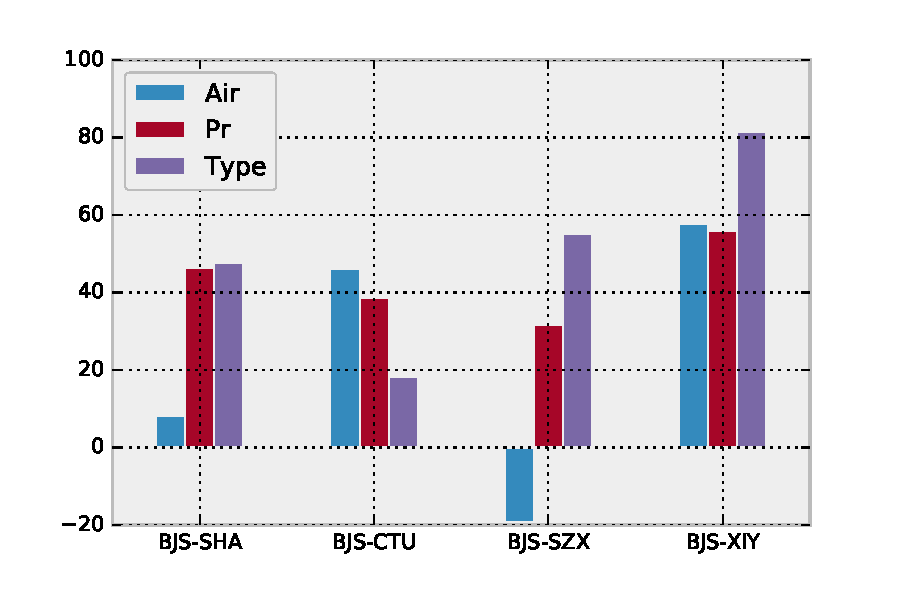
\includegraphics[width=0.75\linewidth]{06/7_res_of_pear_.pdf}
 \bicaption[fig:pear_cof]{相关系数}{用户模型与航线分布相关系数}{Fig}{Pearson Correlation Coefficient between User Model and Distribution over Air Routes}
\end{figure}

图\ref{fig:pear_cof}展示了航空公司、价格等级、飞机型号三个特征与四条航线上特征分布的相关程度。其中纵轴的含义是相关系数百分比。此处使用了北京到西安航线上的用户偏好模型,我们在该航线上对活跃用户(训练订单不少于三单)进行抽样;并计算他们的特征分布模型在这三个维度上与四条航线的相关系数的平均值。从图中可以看出,用户在北京到西安航线上的模型与该航线的特征分布相关程度最高,均远高于其他航线。在三个特征中,相关程度差异最小的是价格等级特征,因为无论在哪条航线上,经济舱、低价机票用户的比例都是最高的;相关程度差异最大的是航空公司特征,这可能与不同航空公司在不同航线的运营策越有关。
在北京-深圳航线,用户模型与航线特征分布呈负相关。我们通过计算相关系数验证了用户模型与航线特征分布的关系。

\subsubsection{航线冷启动用户机票推荐结果分析}

\begin{figure}
 \centering
 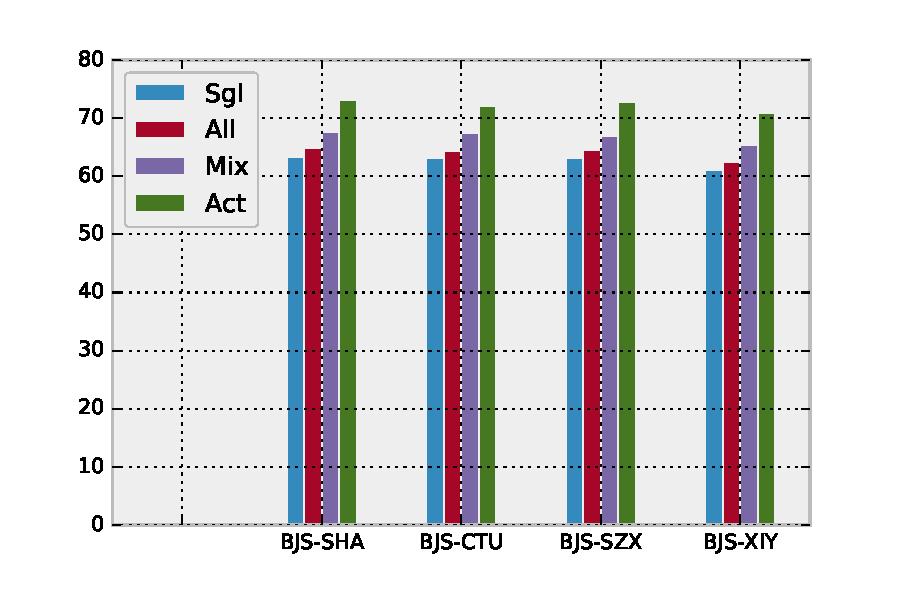
\includegraphics[width=0.75\linewidth]{06/6_res_of_air_cold_rec.pdf}
 \bicaption[fig:cold_rec]{航线冷启动推荐}{航线冷启动用户推荐结果}{Fig}{Mean Accuracy of Recommendation for Air Route Cold Start Users}
\end{figure}

图\ref{fig:cold_rec}展示了在四条航线上的机票推荐结果。其中Act标签代表为该航线活跃用户的单一航线模型推荐结果。可以看到,在每条航线上,活跃用户的机票推荐准确率比非活跃用户提升较多。Sgl标签代表为航线冷启动用户使用单一航线模型的推荐结果;All标签代表为航线冷启动用户使用全航线模型的推荐结果;Mix代表为航线冷启动用户使用修正混合模型的推荐结果。我们得出基本结论是为此类用户使用全航线模型的推荐准确率高于仅使用目标航线模型;而使用修正混合模型具有最高的推荐准确率,只是距活跃用户仍有一定差距。


\section{基于社会关系解决用户冷启动问题}

本节我们分析用户冷启动问题,即该用户的活跃程度较低,在所有航线上的订单数量都很少。因此我们无法使用上一节中选取最优相似航线的方法为用户建立修正混合模型。唯一可行的方法似乎只有使用用户全航线模型进行推荐,但这样同样面临上一节中提到的航线间特征分布差异、用户行为差异的问题。为了有效解决这类问题,我们借助于用户间的社会关系,通过模型迁移来强化非活跃用户的特征分布模型。


\subsection{社会关系的定义}
在现实生活中,社会关系用于描述人与人之间的社会联系,例如家庭、同事、朋友等。在机票推荐情景中,我们无法获得用户之间的在现实中的具体关系,也难以衡量用户之间社会关系的亲疏程度。然而,我们可以通过机票订单数据集挖掘到用户之间的关系,这种关系仅表示用户在机票票务领域的一种连接形态,虽不能反映用户间的现实社会关系,但在解决用户冷启动问题中可以提供一定程度的帮助。

在机票的订购流程中,当用户选定机票后,需要填写乘客的身份信息,包括姓名、证件号等内容,因此进行订票的网站用户不一定是最终的乘客。用户与乘客之间可以是一对一、一对多、多对多这几种类关系;在数据集中,我们通过网站账户的注册ID来识别用户;通过加密过的乘客证件号来识别乘客。如果一个乘客出现在多个用户中,我们称这两个用户具有共同乘客,可以为这两个用户建立社会关系。在共同乘客数量的统计过程中,我们可以使用倒排索引以大幅减少计算开销。在全量订单中统计乘客-用户字典,以乘客为键,乘客出现过的用户集合为值,为集合中的用户两两增加一次共同乘客数量。对所有乘客都执行统计后,
我们就可以得到所有用户的共同乘客数量。

挖掘用户间的社会关系除了依据用户与乘客的对应关系外,乘客之间还有同乘关系。虽然他们没有在同一个用户下订票,却乘坐了同架飞机。如果两个用户同乘飞机超过一次,我们就可以认为两个用户可以建立社会关系。这里我们按同航班号、同起飞日期、同舱位等级的策略来标识同架飞机。因为两个同乘的用户一般不会选择不同的舱位,这里可以大幅减少我们的计算开销;并且我们的目的是根据用户间的社会关系强化用户模型,如果同乘用户的偏好具有较大差异,他们的模型也不应该被相互迁移。

\begin{figure}
 \centering
 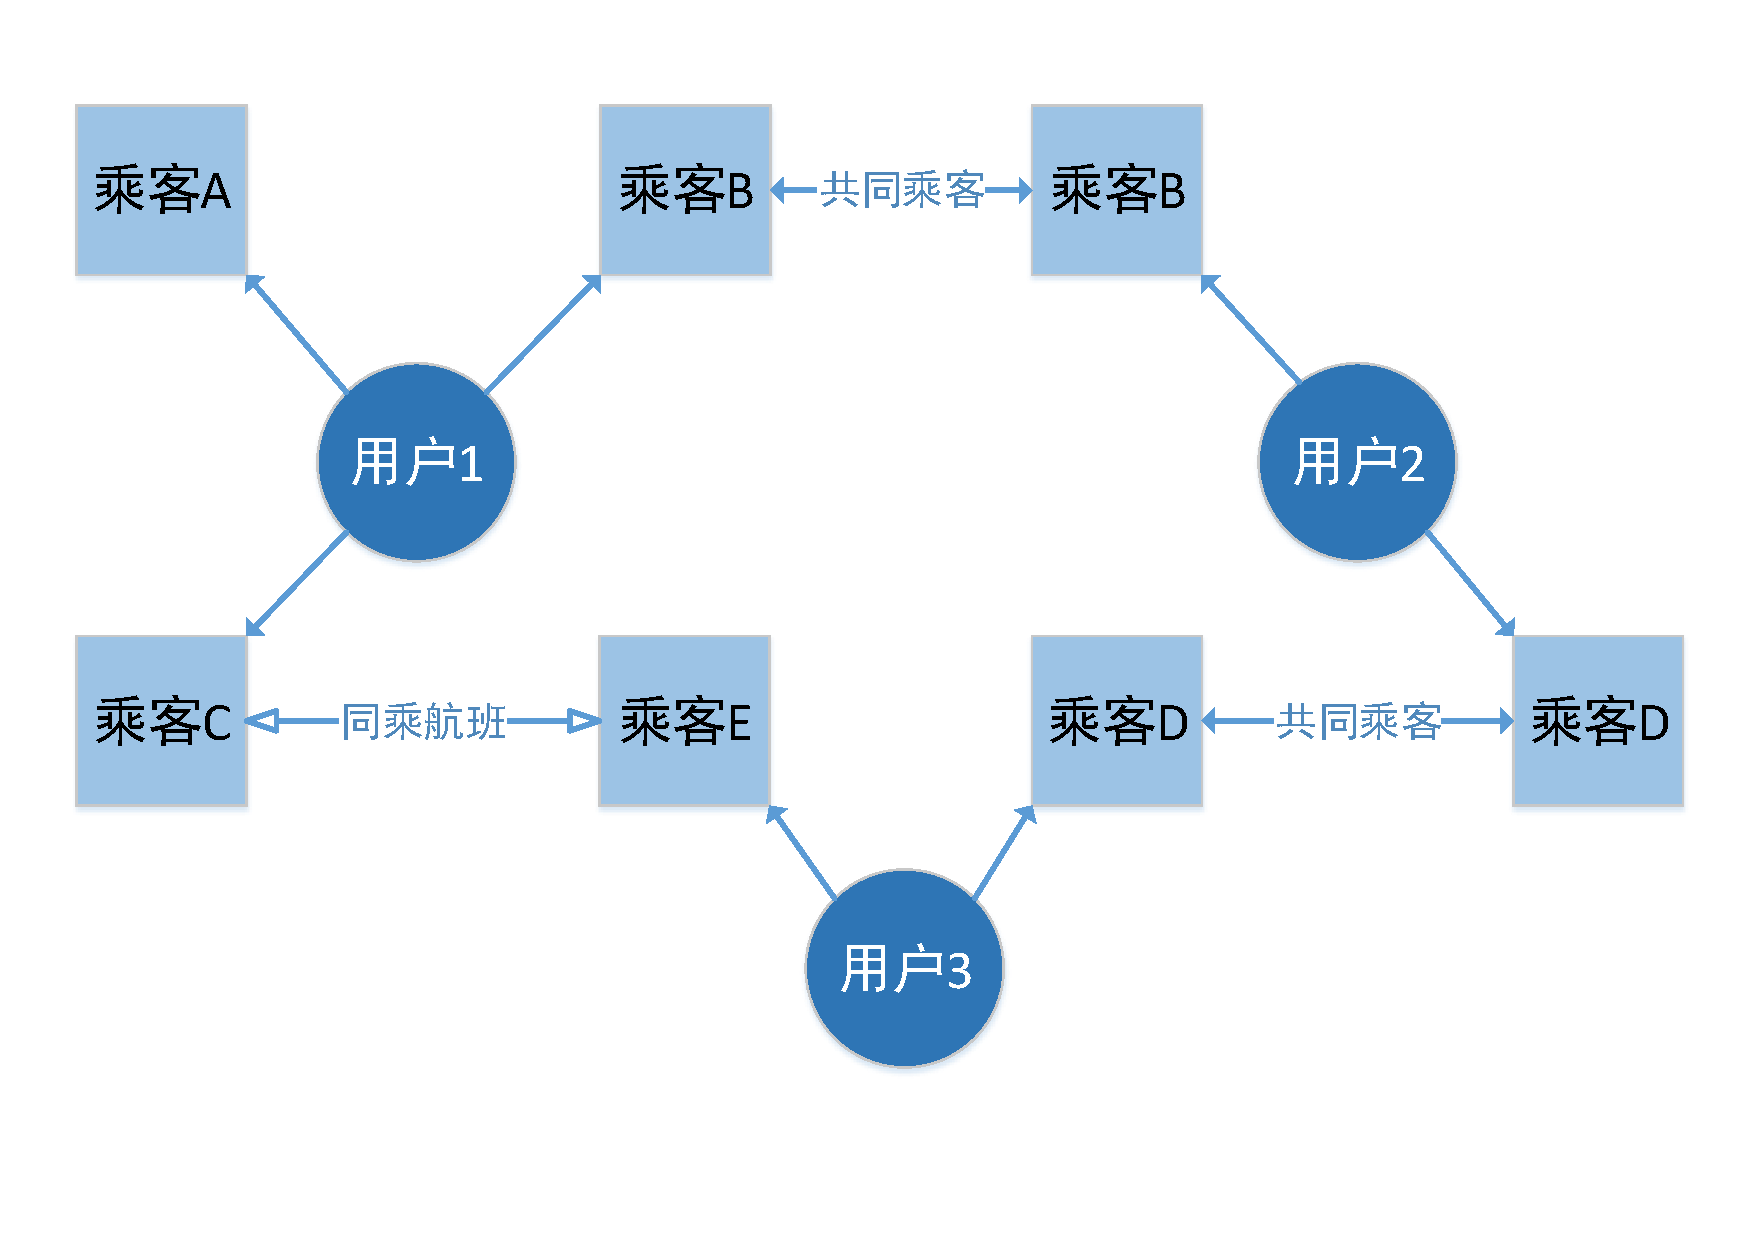
\includegraphics[width=0.75\linewidth]{06/8_model_of_social.pdf}
 \bicaption[fig:social_model]{用户社会关系}{用户间社会关系模型}{Fig}{Model of Social Relationship among Users}
\end{figure}

图\ref{fig:social_model}阐述了从机票订单中挖掘出的用户社会关系模型。图中共有三位用户以及五位乘客。其中用户一为乘客A、B、C订过机票;用户二为乘客B、D订过机票;用户三为乘客D、E订过机票。因此用户一和用户二可以通过乘客B建立社会关系;用户二和用户三通过乘客D建立社会关系。乘客C和乘客E曾同乘飞机超过一次,也可在用户一和用户三之间建立社会关系。

在定义了机票用户之间的社会关系后,我们还需定义计算社会关系紧密程度的衡量规范。当某个冷用户可以与多个用户建立社会关系时,我们可以按照这个衡量规范为其挑选关系最紧密的用户进行模型增强。例如在上图\ref{fig:social_model}中,虽然用户一和用户三都与用户二有共同乘客,但是用户三包含的乘客数少于用户一,我们可以认为用户三与用户二的社会关系紧密度高于用户一和用户二。在选择强化用户二的偏好模型时,用户三有更高的优先级。

\begin{equation}
\label{eq:relation}
	Rela(U_1,U_2) = \log|O_{U2}| \frac{UF(U_1,U_2) + UP(U_1,U_2)}{\sqrt{|P_{U1}|*|P_{U2}|}}
\end{equation}

式\ref{eq:relation}从共同乘客数量和同乘次数两方面衡量了用户间的社会关系紧密度。分子中$UF(U_1,U_2)$代表两个用户的同乘(User-Flight)次数;
$UP(U_1,U_2)$代表两个用户共同乘客(User-Passenger)数量。分母是用户包含的乘客数量乘积,
是一项惩罚项,其含义是当UF,UP数量固定时,一个用户包含的乘客数量越大,这个用户的偏好越不具备代表意义,因此使用这个偏好为冷启动用户进行模型增强的意义很低,我们需要将这类用户与其他用户的关系紧密度定义的尽量小。如果组成两个账户的乘客完全相同,则他们的关系紧密度不小于1;在分子$UF(U_1,U_2)$中,我们不存储同乘次数仅为1次的用户,因为每架飞机都有数百位乘客共同出行过,我们不能认为这些乘客之间都互相具备社会关系。

我们假设U1代表冷启动用户,称为源用户;U2代表需要为U1进行模型增强的候选用户。公式中第一项是候选用户的订单数量取以10为底的对数。正如同我们在解决航向冷启动问题时添加的激励因子,需要保证候选用户不是冷启动用户。

\subsection{增强用户模型}

定义了用户间社会关系以及社会关系紧密度计算公式后,我们就可以针对具有社会关系的冷启动用户进行模型增强。将与该用户建立社会关系的用户集合以社会关系紧密度由高到低进行排序。取排序最靠前的用户为目标用户进行模型增强。

如果候选用户在目标航线上不是冷启动用户,则将候选用户的特征分布模型与源用户的模型线性相加;反正,则采取类似航线冷启动用户的模型修正策略,将候选用户在与目标航线最相似航线上的模型与源用户的模型相加。

\begin{algorithm}
\caption{增强用户模型}
\label{algo:all_cold}
\begin{algorithmic}[1]
\Require
\Statex 用户全航线历史订单 $O$
\Statex 机票特征集合 $F$

\Ensure 
\Statex 增强用户特征分布模型 $D_{amp}$

\State $U \gets getRelatedUsers(u_a)$
\State $Rank\_list \gets \emptyset$
\For { $u \in U$}
\State $Rank\_list.append(Rela(u_a,u)) $
\EndFor
\State $u_o \gets Max(Rank\_list)$
\State $r_o \gets getOptimalRoute(u_o)$
\State $D'[r_o] \gets D[r_o] / M[r_o]$

\State $D_{amp} = Normalize(D[r_a] + D'[r_o])$

\State \Return $D_{amp}$
\end{algorithmic}
\end{algorithm}

算法\ref{algo:all_cold}描述了冷启动用户模型增强的过程。第一步需要获取与该用户建立社会关系的用户集合。然后根据关系紧密度公式挑选出与源用户社会关系最紧密的候选用户。最后将候选用户在目标航线或最优相似航线上的特征分布模型对用户模型进行增强,并将增强后的模型用于机票推荐。

\subsection{实验结果分析}

\subsubsection{实验数据集及评价指标描述}

本节我们验证增强用户模型为冷启动用户进行机票推荐的准确率。仍旧选取北京到上海,北京到成都,北京到深圳,北京到西安这四条航线。选取了在每条航线上订单数量均不超过两单的用户,这些用户还要具备可建立社会关系的其他候选用户。我们为这些用户分别测试单一航线用户模型、全航线用户模型以及增强用户模型的推荐效果。

我们仍旧使用式\ref{eq:a-rec}对每条机票推荐准确率进行评价,
以及式\ref{eq:ma}对每种模型下所有用户的推荐平均准确率进行评价。

\subsubsection{用户社会关系分析}

\begin{figure}
 \centering
 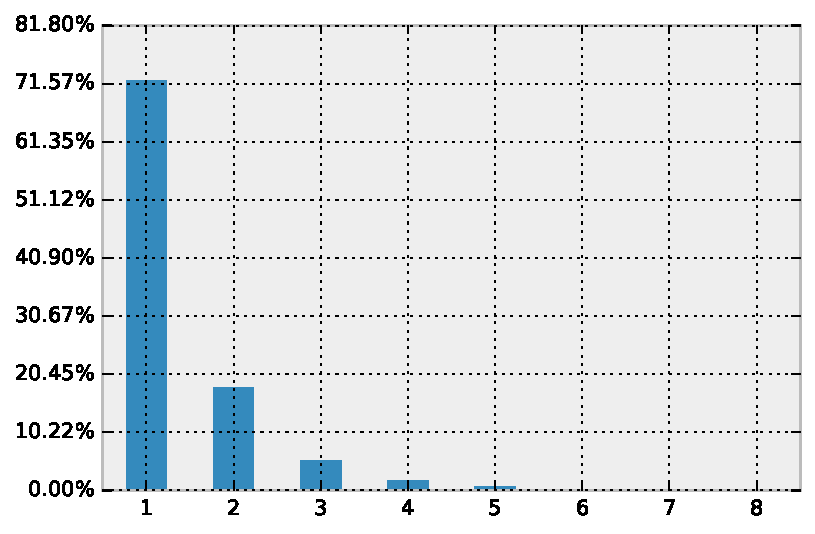
\includegraphics[width=0.75\linewidth]{06/9_same_flight.pdf}
 \bicaption[fig:same_flight]{同乘用户}{具备同乘关系的用户分布图}{Fig}{Users Establishing Relationship with Others for taking Same Flight}
\end{figure}

图\ref{fig:same_flight}描述了通过同乘航班建立社会关系的用户分布图。其横轴代表与一个用户有同乘关系的用户数量。前文提到,具备同乘关系的前提是与其他用户乘坐同一航班超过一次。可以看到,只与一位用户有同乘关系的用户数量占比达到70\%,与两位用户有同乘关系的用户数量占比约18\%左右,与三位以上用户有同乘关系的用户数量占比约10\%。

\subsubsection{冷启动用户机票推荐结果分析}

\begin{figure}
 \centering
 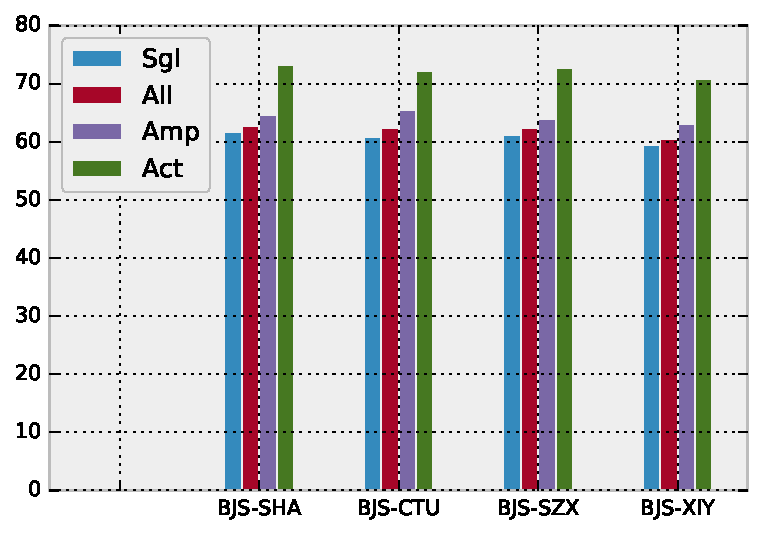
\includegraphics[width=0.75\linewidth]{06/10_res_of_cold_rec.pdf}
 \bicaption[fig:real_cold_flight]{冷启动用户推荐}{冷启动用户推荐结果}{Fig}{Mean Accuracy of Recommendation for Cold Start Users}
\end{figure}

图\ref{fig:real_cold_flight}展示了为冷启动用户在四条航线上机票推荐的结果。同样地Act标签代表为该航线活跃用户的单一航线模型推荐结果。Sgl标签为冷启动用户使用单一航线模型的推荐结果;All标签对应为冷启动用户使用全航线模型的推荐结果;Amp代表为冷启动用户基于社会关系进行模型增强的推荐结果。可以看到,为冷启动用户进行模型增强的机票推荐结果仍优于仅使用用户本身数据的单一航线用户模型和全航线用户模型。验证了具备社会关系的用户之间的偏好模型可以进行迁移,并适用于增强冷启动用户的特征分布模型,最终提高机票推荐的准确率。


\section{本章小结}
本章我们提出并分析了机票推荐场景中的冷启动问题。首先,我们基于机票的几个特征分析了航线间的分布差异及用户行为的差异。然后分析了航线差异对推荐结果的影响,当用户在目标航线上训练订单较少时,学习的特征分布模型具有一定偶然性,因而使用全航线模型的推荐效果好于单一航线模型;随着训练订单数量的增加,单一航线模型的推荐效果好于全航线模型。因此验证了对用户模型分航线的必要性。因而,可能产生几种用户冷启动问题。

第一种是用户在目标航线上的训练订单数量不足,而在别的航线上有一定数量的训练订单。这类用户称为航线冷启动用户。我们的解决策略是关注用户在其他航线上的特征分布模型,通过比较航线间的相似度,选出最优相似航线。提出了模型修正与融合的过程,得到最终的用户修正混合模型。实验结果验证了这种模型的推荐效果好于全航线模型,也进一步证明了为用户进行偏好建模时,使用的数据不一定越多越好。

第二种是用户在所有航线上的训练订单数量都不足,对于这类用户,似乎只能使用全航线模型。但是我们通过分析机票数据发现,用户与乘客并不是严格一一对应的。可以通过用户之间的共同乘客为用户建立社会关系。另外,我们还挖掘了用户间的的同乘关系。结合用户的这两种社会关系,我们提出了增强用户模型的算法,提升了这类用户的推荐效果。

对于不满足构建修正混合模型以及通过社会关系进行模型增强的用户,我们的建议是使用全航线模型进行推荐,推荐效果也会好于单一航线模型。
%# -*- coding: utf-8-unix -*-

\chapter{结合共享账户的机票推荐算法}
\label{chap:share}

本章我们研究机票推荐中的共享账户问题,该问题主要针对一个用户ID包括多个乘客的情况。我们将提出一种算法,可以预测出用户下本次购票的乘客的概率分布,从而学习更具针对性的偏好模型,提升推荐准确率。

\section{机票推荐中的共享账户}

传统推荐系统通常以用户在网站的注册ID(账户)来识别用户,它们一般假定一个用户背后只有一个使用者,即每个用户仅包含一个固定的偏好模型。然而在很多领域,都会发生现实中几个人共同使用一个账户的情景。例如,在购物网站,可能一个家庭共用一个账户,每位家庭成员都可以使用这个账户进行购物;在一般的线旅行票务服务网站,例如机票、酒店、旅游等业务领域,一个账户中也可能会有几个成员,他们可能会为家人、旅伴购票。


第一种情形中,虽然会有几位家庭成员共同使用账户购物,但是服务商无法获取购物者的真实身份信息。而对于第二种情形,如图\ref{fig:fill_id}所示,乘客在订票后会被要求填写身份信息,因此,网站可以获取其真实身份。在机票数据集中,订单包含了每一位乘客的身份信息,包括姓名、性别、年龄、证件号码等。在我们进行数据分析与实验过程中,统一使用加密后的证件号码来代指乘客,既确保了乘客之间无冲突,又保护了乘客隐私。

\begin{figure}
 \centering
 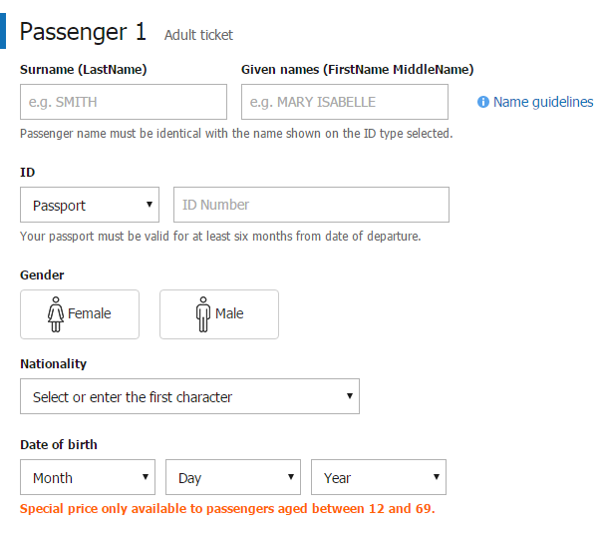
\includegraphics[width=0.7\linewidth,height=0.5\linewidth]{05/1_fill_id.png}
 \bicaption[fig:fill_id]{填写乘客信息}{用户在票务网站填写身份信息}{Fig}{Users Fill in Their Identification on Website}
\end{figure}

通常来说,同一个用户下乘客可能具有较为相似的偏好,但他们之间的差异也不能忽视。如果我们能够利用购票时获取的乘客身份信息为该乘客进行机票推荐,就可以为每位乘客建立特征分布模型,更具针对性的细粒度乘客模型对进一步提升个性化机票推荐准确率可以起到作用。然而,按照业务流程,只有当用户选定机票后才会填写身份信息。在我们进行机票推荐时还无法获取乘客信息。因而,我们需要预测乘客的概率分布。

我们的问题是在共享账户的乘客选购机票时,根据乘客历史行为模式以及当前会话的上下文预测出本次购票的目标乘客。在电子购物网站等无法获得成员真实身份的场景中,为了解决共享账户问题,通常需要设置几个虚拟成员,其中每个成员代表一种偏好模型。虚拟成员的数量可以是固定值,也可以是通过模型计算出的最优值。然而,这类算法通常只分析用户和物品之间的关系,无法利用当前会话中的上下文信息;并且对虚拟成员的预测准确率也无法验证。在机票推荐场景中,对乘客的预测准确率是可以进行验证的。

在机票的乘客预测模型中,我们使用了作者主题模型(ATM)\cite{rosen2004author,steyvers2004probabilistic,rosen2010learning}来分析乘客的行为模型。主题模型是一种生成模型,其主要观点是一篇文档可以抽取出混合的多个主题。作者主题模型在文章-主题的基础上又添加了作者-主题的关系。每个账户独立进行模型训练,可以将每个账户视为一个语料库。账户中出现过的所有乘客视为每位作者,每条机票订单视为一篇文档, 机票中的每个特征以及上下文信息视为预定义的词库。如果出现一张机票有多个乘客的情况,我们将他们视为共同作者。

\section{乘客预测模型}
事实上,主题模型在推荐系统中的得到广泛地应用。例如,在PLSA模型中,每个物品可以视作一个词汇,主题服从对物品的多项式分布,每个主题代表了一种隐性特征,用户的偏好模型服从对主题的多项式分布。用户的每次购买行为都可以被看作从该用户中抽样一个主题,再从该主题中抽取一个词汇的过程。由于机票具有动态属性,很难将不同价格的机票定义为同一个物品;并且每类机票的数量受限于飞机的型号,因此上述pLSA模型很难用到机票推荐领域中。

\subsection{模型描述及表示}

在作者主题模型中,我们用机票在每个特征离散化后的取值来预定义一个词库。这个词库包含了机票在任一特征中所有可能出现的值,使用从0开始的索引来代指每一个词汇。至此,每一张机票都可以表示为词汇的集合,我们将每条订单视作一篇文档,显然,所有订单中的的词汇数量是相同的,每个主题都表示为词汇的多项式分布,每个乘客都表示为主题的多项式分布。因此
ATM模型可以对文档(订单)进行降维。通过ATM模型训练,可以计算出乘客与主题之间的分布参数以及主题与词汇之间的分布参数。表\ref{tab:notation}描述了我们本章使用的符号表。

\begin{table}[!hpb]
\centering
  \bicaption[tab:notation]{符号表}{乘客预测模型符号表}{Table}{Notation for ATM}
\begin{tabular}{|c|c|} \hline
$M$ & 数据集账户数量\\ \hline
$V$ & 词库中单词的数量\\ \hline
$O$ & 一个账户中所有订单\\ \hline
$P$ & 一个账户中所有乘客\\ \hline
$P_i$ & 订单$O_i$对应的乘客集合 \\ \hline
$F$ & 机票特征集合\\ \hline
$K$ & 主题数量\\ \hline
\end{tabular}
\end{table}

对于一个账户$M$,我们获取其中包含的乘客集合$P$。我们使用矩阵$\Theta$来表示每位乘客的主题分布,这个参数矩阵的维度是$|P| \times K$,$K$代表模型主题的数量。$\Theta$以狄利克雷分布作为先验,该先验的超参数是$\alpha$。矩阵$\Phi$可以表示每个主题在词汇上的分布,该矩阵的维度是$V \times K$。$\Phi$同样以超参数为超参数是$\beta$的狄利克雷分布作为先验。通常情况下,超参数不是通过训练得到的,而是根据多次数据实验的经验总结来赋值。本章中,我们将$\alpha$赋值为$50/K$,将$\beta$赋值为$0.01$。

式\ref{eq:dir}描述了狄利克雷分布。其中,带$\Gamma$函数的那一项是常系数。可以发现,狄利克雷分布与多项式分布具有相同的形式。这两个分布是共轭分布。

\begin{eqnarray}
\label{eq:dir}
	Dir(\mathbf{p}|\alpha) & = & \frac{1}{B(\alpha)}\prod_{i=1}^n p_i^{\alpha_i-1} \nonumber \\
	& = & \frac{\Gamma(\sum_{i=1}^n \alpha_i)}{\prod_{i=1}^n \Gamma(\alpha_i)}\prod_{i=1}^n p_i^{\alpha_i-1}
\end{eqnarray}

在训练数据中,一条机票订单的乘客集合是明确的,每张机票的特征内容,即该文档的所有词汇也是明确的;为了训练两个矩阵参数,我们需要为订单中的每个词汇赋予乘客与主题。这两个变量属于隐性变量。首先我们从这条订单的乘客列表中按均匀分布抽取出一位乘客;然后根据乘客-主题参数矩阵抽取出一个主题$Z$,再根据主题-词汇参数矩阵抽取一个单词$w$,我们使用下列流程对生成模型进行数学描述:

\begin{enumerate}
\item 对每个账户中的所有乘客$p$,以狄利克雷先验初始化 $\Theta_p \sim Dir(\alpha)$
\item 对每个主题$t$,以狄利克雷先验初始化 $\Phi_t \sim Dirichlet(\beta)$
\item 对账户下的每条订单$o$
       \begin{enumerate}[fullwidth,itemindent=1em,label=(\alph*)]
       \item $P$ 表示这条订单的乘客集合
       \item 对于订单中的每一个词汇
              \begin{enumerate}[fullwidth,itemindent=2em,label=(\roman*)]
              \item 按均匀分布从$P$中抽取一位乘客 $X_{oi} \sim Uniform(P)$
              \item 从乘客-主题矩阵中抽取一个主题 $Z_{oi} \sim Multi(\theta_{X_{oi}})$
              \item 从主题-词汇矩阵中抽取一个单词 $w_{oi} \sim Multi(\phi_{Z_{oi}})$
              \end{enumerate}
       \end{enumerate}
\end{enumerate}


\begin{figure}[!h]
 \centering
 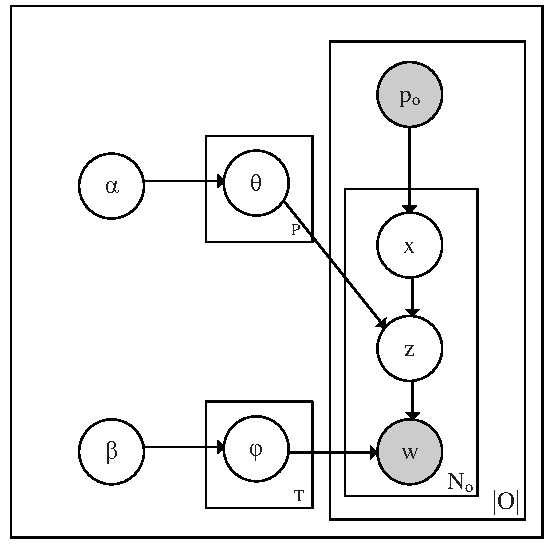
\includegraphics[width=0.45\linewidth]{05/2_graph.pdf}
 \bicaption[fig:pro_graph]{模型概率图}{作者主题模型的概率图}{Fig}{Probability Graph for the Author-topic Model}
\end{figure}

图\ref{fig:pro_graph}展示了作者主题模型的概率图。带阴影的变量是已知变量;其余是未知变量。每个方框代表一个过程,其右下角的数字是这个过程的循环次数。箭头连接线代表了变量间的条件依赖关系。这个图直观、清晰地表现了生成一条订单文档的过程。

\subsection{模型参数推导}
在上节的模型描述中,我们介绍了作者主题模型的两个参数矩阵,分别是包含$P$位乘客的乘客-主题分布参数以及包含$K$个主题的主题-词汇分布。有一些算法可以用来推导这些参数,如EM算法、Gibbs采样\cite{ishwaran2011gibbs}等。传统的EM算法可能会产生局部最优问题,并且这种算法的复杂性较高。本章,我们使用Gibbs采样的算法,这种算法不直接进行参数推导,而通过计算抽取的乘客和主题的后验分布,对参数进行更新。因此计算过程较为简单。


\begin{eqnarray}
\label{eq:all_pro}
P(\mathbf{w}_o | \Theta,\Phi,P) & = & \prod_{i=1}^{N_o}P(w_{oi}|\Theta,\Phi,p_o) 
\nonumber \\
 & = & \prod_{i=1}^{N_o}\sum_{p=1}^{|P|}\sum_{t=1}^{K}P(w_{oi}|z_{oi}=t,\Phi)
P(z_{oi}=t|x_{oi}=p,\Theta)P(x_{oi}=p|p_o) \nonumber \\
 & = & \prod_{i=1}^{N_o}\frac{1}{|P|}\sum_{p \in p_o}\sum_{t=1}^{K}\phi_{w_{oi}t}\theta_{tp}
\end{eqnarray}


式\ref{eq:all_pro}描述了在参数矩阵$\Theta$,$\Phi$和乘客集合$P$的条件下,生成一条机票订单的概率函数。在这个生成模型中,$P(w_{oi}|z_{oi}=t,\Phi)$是在选定主题的条件下,根据主题-词汇分布矩阵抽取单词的概率。
$P(z_{oi}=t|x_{oi}=p,\Theta)$是在选定乘客的条件下,根据乘客-主题分布矩阵抽取主题的概率。$P(x_{oi}=p|p_o)$是乘客集合中以服从均匀分布抽取乘客的概率。该等式可以看作生成一条订单的似然函数。
如果将参数$\Theta$,$\Phi$视为随机变量,我们的目标就是通过参数估计,
使似然函数得到最大后验分布(Maximum A Posteriori,MAP)。 

在Gibbs采样的过程中,为了从联合分布$P(\mathbf{z},\mathbf{x}|\alpha,\beta)$中取样,我们需要为每一个单词$w_{di}$赋值一个主题$z_{di}$以及乘客$x_{di}$。在训练过程中,一个账户下的所有单词都会被取样一次。当所有单词都训练过,称为一个训练批次,通常我们需要将模型训练数个批次。$p(\Theta,\Phi|\mathbf{z},\mathbf{x},\alpha,\beta)$可以根据狄利克雷与多项式分布互成共轭分布的性质来计算。为每个单词抽取的乘客、主题可以使用下式进行计算:

\begin{eqnarray}
\label{eq:pro_pass_top}
P(x_{oi}=p,z_{oi}=t|w_{oi}=w,\mathbf{z}_{-oi},\mathbf{x}_{-oi},\mathbf{w}_{-oi},\alpha,\beta,p_o) \nonumber\\
\propto \frac{C_{tp}^{TP}+\alpha}{\sum{t'}C_{t'p}^{TP}+T\alpha}\frac{C_{wt}^{WT}+\beta}{\sum_{w'}C_{w't}^{WT}+W\beta}
\end{eqnarray}

式\ref{eq:pro_pass_top}代表为订单$o$的第$i$个单词赋予乘客$p$和主题$t$的概率。$C^{WT}$ 是单词-主题分布矩阵,其每行对应一个单词,每列对应一个主题,每个元素代表当前单词被赋予当前主题的次数。$C_{wt}$是除了当前单词之外,单词$w$被赋值到主题$t$的次数。$C^{TP}$是主题-乘客分布矩阵,其每行对应一个主题,每列对应一个乘客,矩阵中每个元素代表该乘客在当前主题包含的单词个数。$C_{tp}$代表乘客$p$在主题$t$生成的词汇个数,同样排除了当前单词。我们可以根据抽样的过程对主题-词汇分布参数以及乘客-主题分布参数进行更新:

\begin{equation}
\label{eq:es_the}
\theta_{tp} = \frac{C_{tp}^{TP}+\alpha}{\sum{t'}C_{t'p}^{TP}+T\alpha}
\end{equation}

\begin{equation}
\label{eq:es_phi}
\phi_{wt} = \frac{C_{wt}^{WT}+\beta}{\sum_{w'}C_{w't}^{WT}+W\beta}
\end{equation}

式\ref{eq:es_the}和式\ref{eq:es_phi}分别两个参数的更新公式。$\theta_{tp}$是主题$t$在乘客$p$上的概率分布;$\phi_{wt}$是单词w在主题t上的概率分布。在每次取样后,
需要为每条订单更新单词-主题列表$T$以及单词-乘客$P$列表,其中$T[o][i]$代表在订单$o$中第$i$个单词的主题;$P[o][i]$代表在订单$o$中第$i$个单词的作者。因此,在参数推导的过程中,
我们需存储上文提到的$C^{TP}$和$C^{WT}$两个矩阵,以及每条订单中每个单词的主题和乘客两个列表。


模型训练主要包括三个步骤,分别是初始化,取样以及参数更新。在初始化过程中,我们为账户中每条订单的每个词汇随机分配主题和乘客。然后我们需要统计词汇表中每个单词被赋予某个主题的次数以及每个乘客在每个主题下的词汇的个数。在每次取样过程中,我们根据式\label{eq:p_xz}为语料库中的每个单词计算每个主题以及乘客的联合概率分布。我们根据概率为该单词采样新的主题和乘客。在几个批次的迭代训练后,可以根据式式\ref{eq:es_the}和\ref{eq:es_phi}对参数矩阵$\Theta$,$\Phi$进行更新。

在最差情况下,每批参数估计的时间复杂度为$O(NK|P|)$。其中$N$是一个账户下所有订单的总词汇数量。$|P|$是该账户下乘客最多的订单中乘客的数量,一般不会很大,与订单的总词汇数量相比可以视作常量。$K$是模型的主题数量。主题数量的取值不是固定的,我们可以在实验中确定最适合机票推荐业务中,乘客预测模型的数量。在模型迭代过程中,$|P|$以及$K$都可以看作常量,因此,使用Gibbs采样训练ATM模型的时间复杂度可以看作与总订单词汇数量$N$呈线性关系,可以用在大量用户数据的训练任务中。

\begin{algorithm}
\caption{Training of ATM}
\label{algo:atm_train}
\begin{algorithmic}[1]
\Require
\Statex Word list of user's historical flight orders $W$

\Ensure 
\Statex Passenger-Topic Matrix $\Theta$
\Statex Topic-Word Matrix $\Phi$

\State $nak , nkv, nak\_sum, nkv\_sum \gets 0$
\State $pl , tl \gets 0$
\For{$o \in W$}
\For{$w \in o$}
\State Pick a topic $t$ and a passenger $p$ uniformly;
\State passenger-topic count $nak[p][t] += 1$;
\State passenger-topic sum $nak\_sum[p] += 1$;
\State topic-word count $nkv[t][w] += 1$;
\State topic-word sum $nkv\_sum[t] += 1$;
\State word-topic list $tl[o][w] = t$
\State word-passenger list $pl[o][w] = p$
\EndFor
\EndFor
\While {not reach iteration limit}
\For{$o \in W$}
\For{$w \in o$}
\State $nak[p][t] -= 1, nak\_sum[p] -= 1$;
\State $nkv[t][w] -= 1, nkv\_sum[t] -= 1$;
\State Sample a new passenger $p'$ and topic $t'$ by Eq \ref{eq:pro_pass_top};
\State $nak[p'][t'] += 1, nak\_sum[p'] += 1$;
\State $nkv[t'][w] += 1, nkv\_sum[t'] += 1$;
\State $tl[o][w] = t', pl[o][w] = p'$;
\EndFor
\EndFor
\EndWhile
\State Calculate $\Theta,\Phi$ by Eq \ref{eq:es_the},\ref{eq:es_phi};
\State \Return $\Theta,\Phi$;
\end{algorithmic} 
\end{algorithm}

算法\ref{algo:atm_train}描述了ATM模型的训练过程。该过程的输入是账户下历史订单根据预定义词库转化的词汇表;输出是两个参数矩阵。其中第1至13行是模型初始化过程;其中第14至25行是使用Gibbs取样过程,每次取样将单词的乘客和主题进行更新,在计算过程中,我们增加了两个矩阵存储中间变量的结果;最后更新$\Theta$和$\Phi$两个参数。

\subsection{使用ATM模型进行乘客预测}

上一节我们介绍了在机票推荐领域中作者-主题模型的训练过程。我们首先定义一个词库,将账户下所有订单用作训练,并最终得到参数矩阵$\Theta$和$\Phi$。我们的目的是利用ATM模型,预测当前会话中账户下所有乘客购票概率分布。该问题在本质上属于分类问题,我们可以计算出每位乘客的购票概率,按概率将乘客进行排序。

\begin{equation}
\label{eq:pred_pass}
p(x=p|o_n,\Theta,\Phi) \propto p(p)\prod_{w \in o_n}\sum_t p(t|w)p(w|t,p)
\end{equation}

式\ref{eq:pred_pass}的含义是在参数$\Theta$,$\Phi$的条件下,词汇集合$o_n$属于乘客$p$的的概率,相当于$p$属于订单$o$的乘客的概率。第一项的含义$p(p) = |O_p| / |O|$,$|O_p|$是训练集中乘客$p$参与的订单数量;$p(w|t,p)$是在给定主题和乘客的条件下,取样单词$w$的概率,由于从乘客中采样主题与从主题中采样单词的过程相互独立,因此$p(w|t,p) = p(t|p) \times p(w|t)$。$p(t|w)$代表单词$w$被赋予主题$t$的概率,可以通过迭代完成后的$C^{WT}$矩阵计算出来。

在乘客预测过程中的还有一个问题需要注意。我们在训练模型时可以使用订单的全部特征内容作为词汇列表;然而在机票推荐场景下,我们无法获得用户将要选购的机票的所有特征内容,因此不能用与训练数据一样的词汇表。因此,我们需要挖掘更多可能获取的特征,如起飞城市、到达城市、订票提前天数、登录网站的时间、IP地理位置等信息;以及用户行为上下文,包括搜索、点击、筛选等行为。因此我们在训练模型时,除了收集机票的特征,还需要将这些信息也转化为词汇,一并参与训练。

获取了每位乘客的概率分布后,为了针对乘客进行建立更细粒度的偏好模型,我们需要提供确切的参与该订票会话的乘客列表。平均每位乘客的概率是$\frac{1}{|P|}$,而我们只取概率超过平均概率的乘客。将这部分乘客视作参与本次订票的乘客集合。

至此,我们使用作者-主题模型对当前会话的乘客进行了预测,预测过程总体分为两个步骤。第一步,我们生成了一个预定义词库,使用Gibbs采样迭代训练了模型参数矩阵$\Theta$和$\Phi$;第二步,我们使用公式\ref{eq:pred_pass}为当前会话的乘客概率分布进行预测,并最终决定了参与本次订单的乘客集合。

\section{结合乘客预测的机票个性化推荐}
上一节介绍了机票推荐中的乘客预测算法,本节我们将乘客预测结合到个性化机票推荐中。旨在细化偏好模型的粒度,为乘客建立更有针对性的特征分布模型。进一步提升推荐准确率。

\begin{figure}
 \centering
 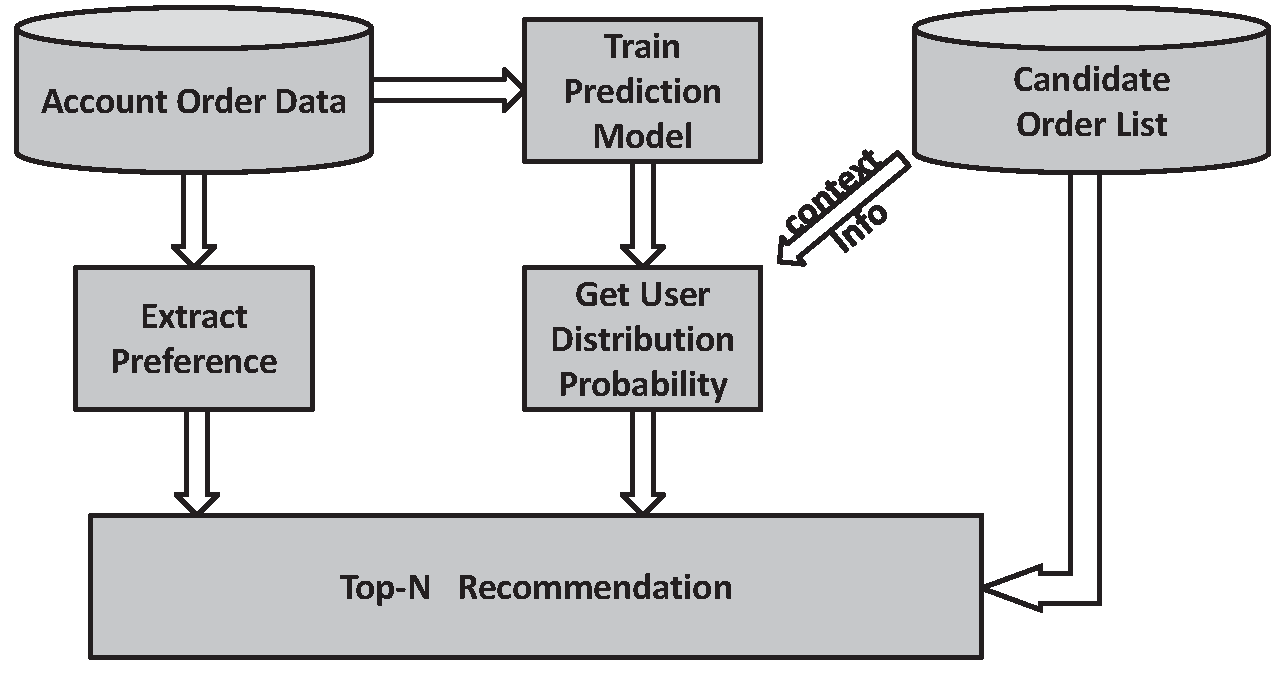
\includegraphics[width=0.6\linewidth]{05/3_overview.pdf}
 \bicaption[fig:over_pr]{预测推荐概览}{结合乘客预测的机票推荐概览}{Fig}{Overview of Passenger Prediction based Recommendation}
\end{figure}

图\ref{fig:over_pr}是结合乘客预测的机票推荐流程概览图。我们的数据源是存储在数据仓库中的用户机票订单数据。一方面我们可以利用这部分数据进行作者-主题模型训练,将训练后的模型用于乘客预测;另一方面,这部分数据还用来构建表示用户偏好的特征分布模型,这里我们不根据账户ID为粒度进行建模,而是为账户中每一位乘机人建立模型。这两个部分都是可以进行离线计算的。此外我们还结合在用户购票会话中的上下文信息,进行乘客预测;并结合乘客预测和机票推荐的结果,对候选机票列表进行排序,得到最终推荐结果。

然而,每位用户的乘客预测模型并不是一成不变的。用户每购买一次机票,我们都需要为该账户更新ATM模型,将本次订单包括进去。最佳的更新策略是每添加一条新的订单时,都重新训练模型,但这会带来计算效率低下的问题。我们可以使用一种蒙特卡洛算法进行更新,这种更新策略只关注新订单中的词汇,因此我们可以快速为新订单中的词汇赋值乘客与主题。首先,我们将该条订单中的词汇随机赋予乘客与主题;然后我们对新订单中的词汇按照式\ref{eq:pro_pass_top}重新取样乘客和主题,并更新矩阵$C^{TP}$和$C^{WT}$,最终更新两个参数矩阵。由于新订单中词汇较少,只需要十次左右的迭代过程就可以完成训练。

获取到乘客的概率分布并选取出参与当前订单的乘客后,我们将这些乘客的特征分布模型读取出来,并进行融合。融合的策略可以按照计算出的乘客分布概率进行加权,我们除了考虑乘客分布概率外,还需要考虑乘客的订单总量,这里我们给出乘客特征分布模型的融合策略:
\begin{equation}
	\label{eq:dis_com}
	\mathbf{D'} = \sum_{p \in P'} p(x = p|o_n,\Theta,\Phi) * \log |O_p| * \mathbf{D_p}
\end{equation}

式\ref{eq:dis_com}给出了多乘客的特征分布融合公式。其中$P'$是本次会话预测的参与乘客集合。我们为每位乘客赋予的权重是该乘客的参与概率以及该乘客参与的订单数量取以$10$为底的对数。得到了融合的特征分布模型后,我们就可以将之用在机票推荐上。

\section{实验结果分析}

本节我们对前几节提出的基于作者-主题模型的乘客预测及机票推荐算法进行实验评估与分析。

\subsection{实验数据集与评价指标}

\subsubsection{实验数据集描述}
我们的实验数据集是用户在多航线上的机票订单数据。数据以用户ID区分每个账户,以订单ID区分每条订单,以加密后的乘客证件号区分订单中的每位乘客。数据集引入乘客字段后,每个订单ID可能对应多条订单数据副本,每个副本之间唯一的差别就是乘客ID字段。我们取乘客数量在$2$至$5$人的网站账户,如果乘客数量过多,这个账户可能是代理账户,并且每位乘客订单比重很小。不适合用于训练乘客预测模型。

除了从数据仓库中直接拉取的账户训练数据外,我们还生成了一份虚拟账户数据。在一些共享账户推荐问题的研究中会用到虚拟账户数据。一般的做法是将两个或多个账户的数据合并为一个账户。由于账户的偏好模型具有较为明显的差异,在研究中可以将每个真实账户的偏好模型视作虚拟账户中的一个成员。使用这类数据可以充分挖掘共享账户中的特征差异。另外,一般的共享账户问题缺少准确的账户成员信息,无法验证实验结果,而使用虚拟账户数据同时可以作评价实验结果的依据。

在我们的问题中,每位乘客的身份信息是明确的,我们生成虚拟账户数据的目的是探究乘客间的偏好差异对乘客预测以及机票推荐准确率的影响。我们的生成策略是在随机的两个账户中取一位乘客,并将这两位乘客合成一个乘客。如果两位乘客有同一个航班在同一起飞日期的订单,我们随机删除一条订单。

\subsubsection{乘客预测与机票推荐的评价指标}

对于一条订单数据,乘客预测的评价指标是预测正确的乘客数量,我们使用下式来评价乘客预测的准确率:
\begin{equation}
\label{eq:pass_acc}
Acc(o_i) = \frac{P' \cap A}{\sqrt{|P'| \times |A|}}
\end{equation}

式\ref{eq:pass_acc}中,$P'$是我们预测的乘客列表; $A$是本条订单实际乘客列表,对每条测试数据而言是一个固定值。其中分子项是预测乘客与实际乘客的交集;分母项是预测乘客与实际乘客各自数量的乘积,是一项惩罚项。可以看出,如果预测乘客与实际乘客集合完全相等,则准确率是$1$;如果预测乘客没有命中任
何一位实际乘客,则准确率是$0$。在预测准确的乘客数量固定的前提下,预测乘客越多,准确率越低。
对于机票推荐,我们使用式\ref{eq:a-rec}对每条机票推荐准确率进行评价,
以及式\ref{eq:ma}对每种模型下所有用户的推荐平均准确率进行评价。除此之外,考虑到实际应用场景。
我们还增加了$Top-N$评价指标:

\begin{equation}
\label{eq:topn}
top-N = \frac{\sum_{i=1}^{|M|}|top-N(u_i) \cap O_{u_i}|}{|M|}
\end{equation}

对一次推荐而言,如果推荐列表中前$N$条候选机票包含了用户实际选择的机票,则认为推荐成功,否则就认为推荐失败。$Top-N$准确率是对所有推荐的平均准确率。可以直观衡量推荐的效果。


\subsection{乘客预测准确率}
本小节我们对乘客预测的准确率进行评价。我们为每个账户训练作者-主题模型,并在测试订单上进行乘客预测。
\begin{figure}[!h]
\centering
\subfigure[真实账户乘客预测准确率]{
 \label{fig:pre_acc_r}
 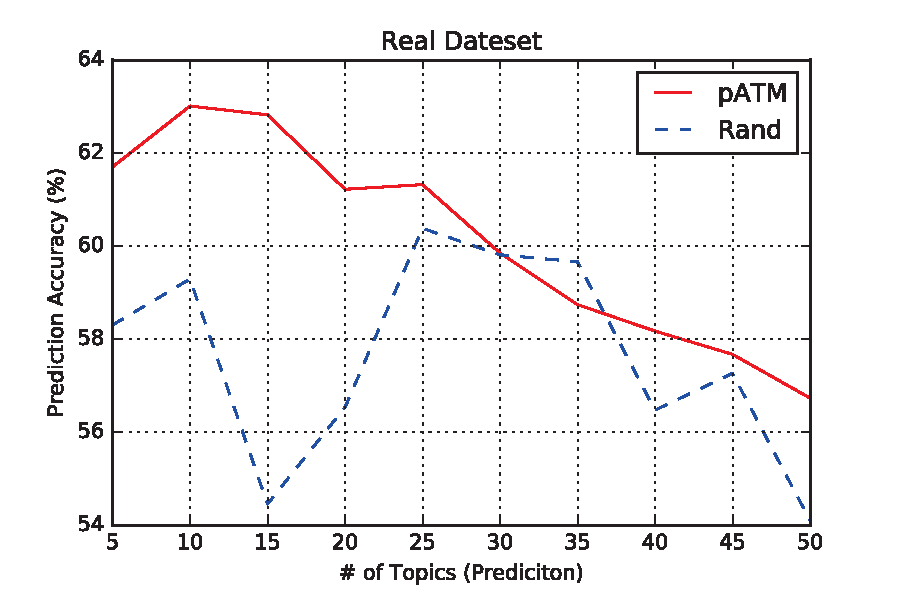
\includegraphics[width=0.49\linewidth]{05/4_pred_real.pdf}}
\subfigure[虚拟账户乘客预测准确率]{
 \label{fig:pre_acc_a}
 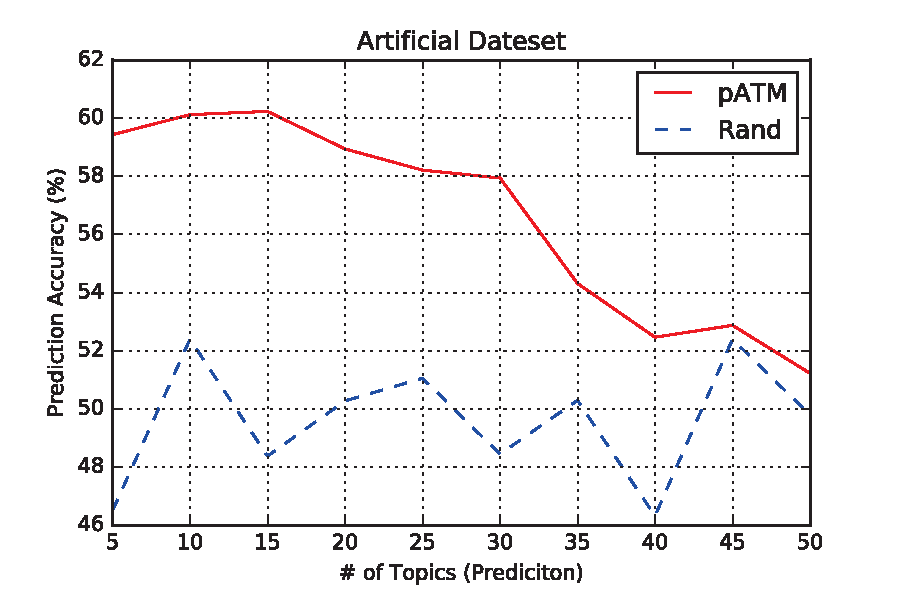
\includegraphics[width=0.49\linewidth]{05/5_pred_arti.pdf}}
\bicaption[fig:pred_acc]{乘客预测}{两个数据集上乘客预测准确率}{Fig}{Mean Accuracy for Passenger Prediction on Datasets}
\end{figure}

图\ref{fig:pred_acc}展示了乘客预测的实验结果。其中图\ref{fig:pre_acc_r}是在真实账户数据集的实验结果;图\ref{fig:pre_acc_a}是在虚拟账户数据集的实验结果。
其中,横轴是主题数量,范围从$5$到$50$共$10$个取值。进行乘客预测的两种方法分别是作者-主题模型(pATM)预测以及随机预测(Rand)。在随机预测中,我们同样取$10$个随机值。

可以看到,在真实账户数据集中,随机乘客预测的平均准确率在$57\%$左右,而ATM模型的最高预测准确率是$63\%$。在虚拟账户数据集中,随机乘客预测的平均准确率在$50\%$,因为每个虚拟账户只有两位乘客,而我们每次仅选取一位乘客;并且每条订单的乘客数量也是$1$。而ATM模型的最高预测准确率是$60\%$。可以看到,在真实数据集中的乘客预测准确率略高与虚拟数据集。
其原因是预测准确率和预测乘客以及实际乘客的数量有关,在不同的数据集上的基准值也不相同。而随机算法在一定程度上可以反映出这个基准值。因此我们的主要标准是衡量ATM模型准确率对随机预测算法的提升。

在虚拟账户上准确率的提升高于真实帐户。因为虚拟账户的乘客间差异更大,更有利于提取各自的特征。在真实账户数据集,乘客预测的准确率对比与随机预测有所提升。在两个数据集上,预测准确率都与主题的数量相关。当主题数少于$15$时,预测准确率保持在较高的水平;而随着主题数目的增加,预测准确率有所下降;通过观察训练参数我们发现,过多的主题数会增加参数的稀疏性,这会影响到预测准确率。在两个数据集上,预测准确率都是在主题数为$10$的情况下达到最高值,这证明了ATM模型对同构的文档具有较稳定的表现。
在下一小节机票推荐部分中,我们将乘客预测模型的主题数量固定为$10$。


\subsection{机票推荐准确率}
本小节我们为账户(用户)进行机票推荐,虽然已经训练了乘客预测模型,并且进行了乘客粒度的特征分布模型学习。在实际应用中,机票推荐还是在用户粒度进行的。我们将从基于排序的推荐准确率和$Top-N$准确率两个角度进行衡量。

\begin{figure}
\centering
\subfigure[真实账户推荐准确率]{
 \label{fig:pre_rec_r}
 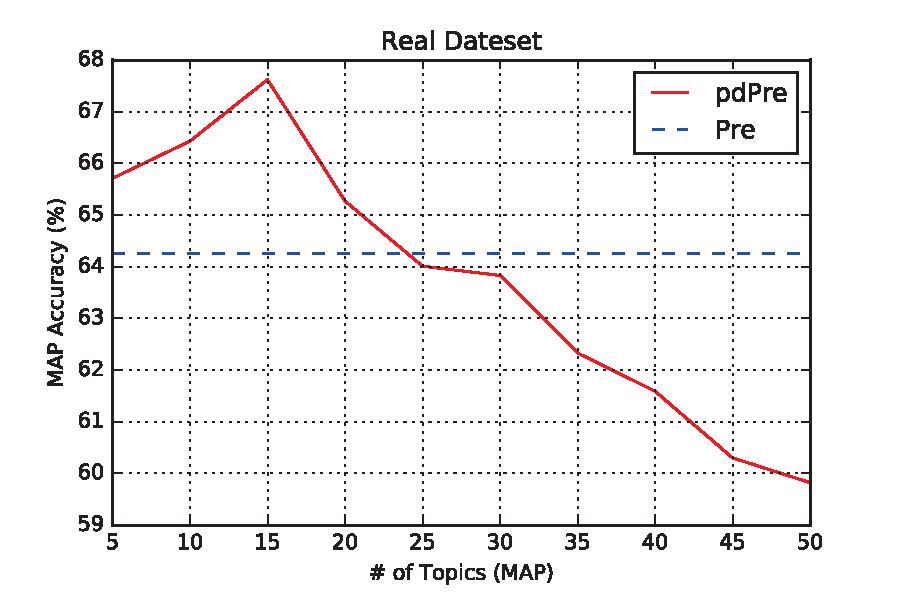
\includegraphics[width=0.49\linewidth]{05/6_rec_rank_r.pdf}}
\subfigure[虚拟账户推荐准确率]{
 \label{fig:pre_rec_a}
 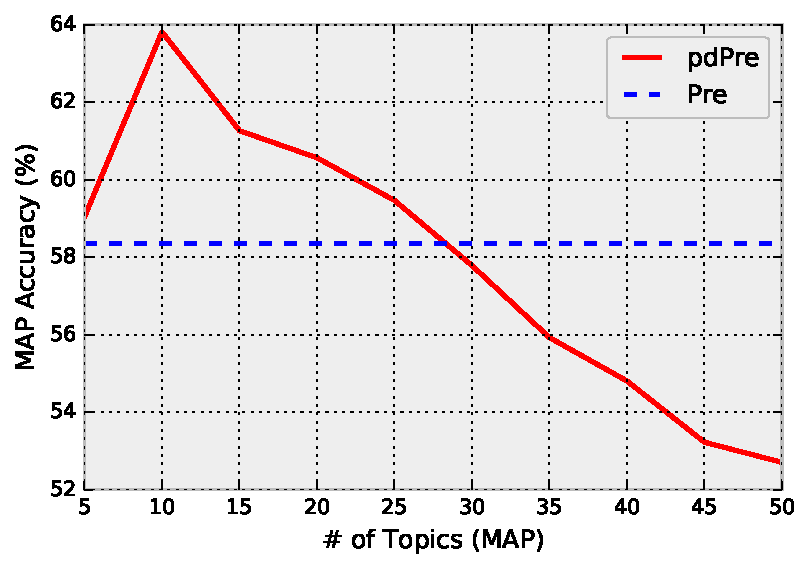
\includegraphics[width=0.49\linewidth]{05/7_rec_rank_a.pdf}}
\bicaption[fig:pred_rec]{机票推荐}{两个数据集上机票推荐准确率}{Fig}{Mean Accuracy for Flight Ticket Recommendation on Datasets}
\end{figure}

图\ref{fig:pred_rec}展示了机票推荐的实验结果。其中图\ref{fig:pre_rec_r}是在真实账户数据集的推荐结果;图\ref{fig:pre_rec_a}是在虚拟账户数据集的实验结果。
其中,横轴是主题数量。进行机票推荐的两种方法分别是结合乘客预测的推荐(pdPre)以及不使用乘客预测的推荐(Pre)。可以看到,推荐结果随着主题数量的变化有较大的波动。并且其变化趋势与乘客预测准确率较为吻合。当主体数量在10到15时,推荐准确率达到峰值;当主题数量在$25$到$30$以上时,推荐效果反而差于不进行乘客预测的推荐。因为此时进行乘客预测的准确率较低,而无法做出有针对性的乘客模型融合。另外,在虚拟数据集上机票推荐准确率低于真实数据集。因为由不同账户抽取出的乘客偏好会有较大差异,如果将其视作一个账户进行偏好建模,会影响机票推荐效果。同样,虚拟数据集对推荐效果的提升程度高于真实数据集。由此我们可以得出结论:在较高的乘客预测准确率的保障下,乘客间的差异越大,结合乘客预测的机票推荐准确率提升越大。


\begin{figure}
\centering
\subfigure[真实账户推荐Top-N准确率]{
 \label{fig:pre_top_r}
 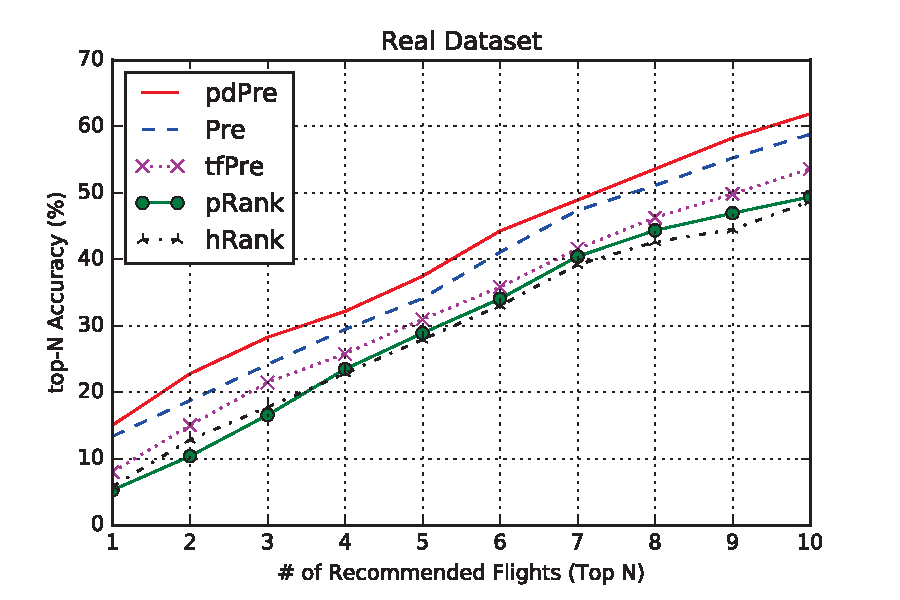
\includegraphics[width=0.49\linewidth]{05/8_rec_top_r.pdf}}
\subfigure[虚拟账户推荐Top-N准确率]{
 \label{fig:pre_top_a}
 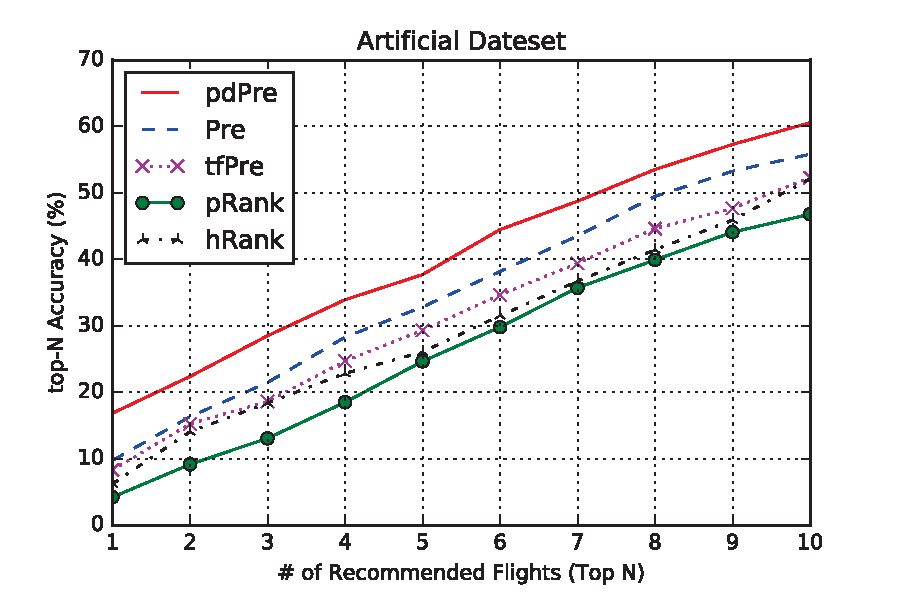
\includegraphics[width=0.49\linewidth]{05/9_rec_top_a.pdf}}
\bicaption[fig:pred_top]{机票推荐Top-N}{两个数据集上机票推荐Top-N准确率}{Fig}{Top-N Accuracy for Flight Ticket Recommendation on Datasets}
\end{figure}

图\ref{fig:pred_top}展示了机票推荐的实验结果。其中图\ref{fig:pre_top_r}是在真实账户数据集的推荐结果;图\ref{fig:pre_top_a}是在虚拟账户数据集的实验结果。在该实验中,我们将ATM模型的主题数量固定在10。
其中,横轴是$Top-N$策略中推荐机票的条数。在$Top-N$方法中,我们一并计较了第三章中提到的基于低价排序(pRank)和热门程度(hRank)排序的推荐准确率。可以看到,总体上机票推荐准确率与推荐的数量呈正比例关系。几种基于基础业务策略的机票推荐准确率与基于用户特征分布模型的推荐准确率有较大的差异。并且推荐机票数量从$1$到$10$,结合乘客预测的机票推荐(pdPre)都比不进行乘客预测的机票推荐(Pre)具有更高的准确率。同时可以看到,
在虚拟数据集上的推荐准确率提升高于真实数据集。两种衡量指标表明,结合用户预测的机票推荐算法在单一的用户特征分布模型基础上进一步提升机票推荐的准确率。并且账户下乘客的偏好差异越大,对推荐效果提升越明显。


\section{本章小结}

本章我们研究了机票用户中的乘客共享账户问题。并基于可以获取账户成员真实信息的场景提出了使用作者-主题模型的乘客预测模型。首先我们预定义了机票特征及上下文词库。在模型训练过程中,我们将每个账户的所有订单作为一个语料库,每条订单作为一个文档,订单的特征取值区间作为一个单词。使用Gibbs取样进行参数推导。并就当前会话的上下文信息给出乘客预测结果。

得到乘客预测结果后,我们将乘客预测结合到机票推荐流程中。我们介绍了推荐流程的概况以及为用户更新ATM模型的过程。使得该模型具有实际应用价值。在实验章节,我们对乘客预测和结合乘客预测的机票推荐进行了数据实验并分析了实验结果。可以说明,ATM模型对乘客预测的准确率有较好的提升效果,并且结合了乘客预测的特征分布模型可以提升机票推荐的准确率。
%# -*- coding: utf-8-unix -*-

\chapter{结合隐性特征的机票推荐算法}
\label{chap:latent}

我们在前几章中介绍了建立特征分布模型表达用户对机票的偏好。为用户建模的过程分为两步,首先从机票数据字段中抽取能反映机票主要内容的显性特征,再根据用户在每个特征内容上的选择分布进行用户建模。本章,我们结合机票的隐性特征建立用户偏好模型,并进行个性化机票推荐。

\section{用户出行性质对机票推荐准确率的影响}

我们将第三章中提出的用户特征分布模型进行上线部署并进行了一段时间的A/B测试对照实验。实验将用户随机分流,一部分用户(实验组)看到的候选机票列表是经过结合其偏好模型进行重排序过后的候选航班展示页。对于航线冷启动用户,我们在线上生产环境中采取了特征打分的原则并提供多样性推荐;其他用户(对照组)看到的是原版展示页。实验的主要观测指标是用户转化率,即订购机票的用户占浏览过机票用户总数的比例。A/B测试证实,实验组比对照组的转化率有所提升,但在周末和节假日时,实验组的转化率有所下降。我们通过分析发现,主要有两方面的原因。

\begin{figure}
 \centering
 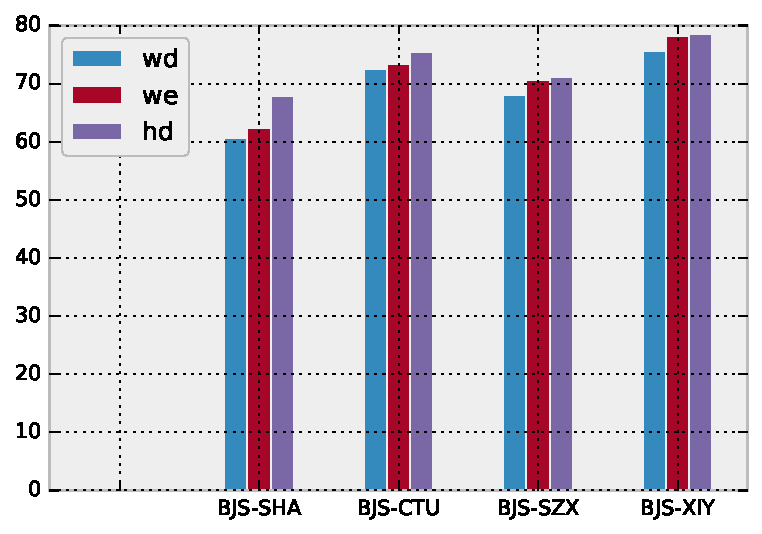
\includegraphics[width=0.6\linewidth]{04/1_inac_count.pdf}
 \bicaption[fig:inac_per]{冷启动用户占比}{不同起飞日期冷启动用户占比}{Fig}{Percentage of Inactive Users at Different Takeoff Date}
\end{figure}

图\ref{fig:inac_per}展示了四条航线在不同起飞日期航线冷启动用户占比。我们将起飞日期分为工作日(wd)、周末(we)和节假日(hd)。可以看到,不同航线上的冷启动用户比例总体有差距。北京-上海和北京-深圳的航线冷启动用户数量处于较低比例;北京-成都和北京-西安的航线冷启动用户数量处于较高比例。对每条航线而言,工作日的航线冷启动用户占比最低;周末和节假日的航线冷启动用户占比都较高,并且比例很接近。其中以北京-上海航线的工作日和节假日的冷启动用户比例差异最大。可以发现,非活跃用户比例差异的是第一个原因。在周末和节假日,航线非活跃用户比例增加,导致推荐效果的差异。第二个原因与用户行为变化相关。我们主要关注用户的出行性质。

用户的出行性质多种多样,如出差、参会、探亲、旅游等。总体来说可以分为商务性质和个人性质。对于出行性质是商务的乘客由于其行程安排及工作单位的差旅政策等因素,可能会更多地关注起飞时间、航空公司等特征,而对价格,舱位等特征关注较少;对于出行性质是个人的乘客,则更关注价格、退改签政策等特征。即使对于同一位用户,如果其出行性质不同,那么在购买机票时的关注点也会不同,从而产生用户行为的变化。用户的出行性质是一个无标签分类问题,它不能直接体现在订单数据中。因而我们无法对这个问题进行实验验证。但是我们可以通过直接对比推荐准确率,分析用户的行为是否产生变化。

\begin{figure}[!h]
 \centering
 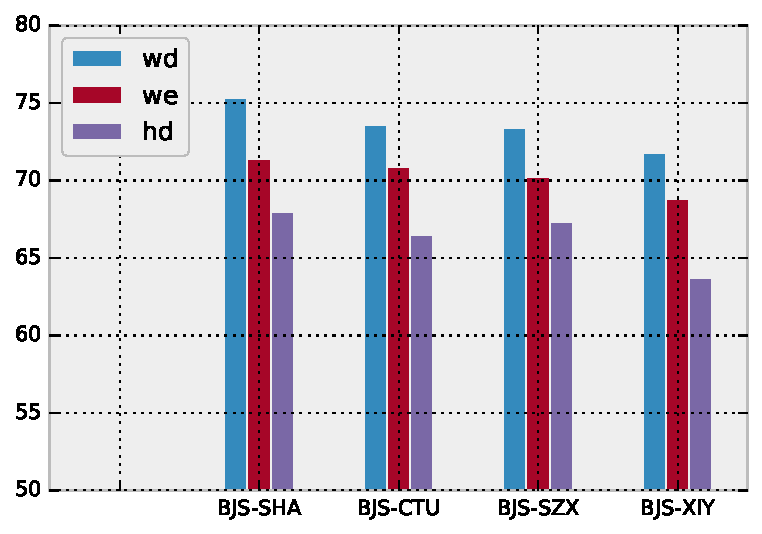
\includegraphics[width=0.6\linewidth]{04/2_wehd_rec.pdf}
 \bicaption[fig:at_rec]{分期机票推荐}{不同起飞日期机票推荐平均准确率}{Fig}{Mean Accuracy of Flight Recommendation at Different Takeoff Date}
\end{figure}

我们同样将测试订单按起飞日期分为工作日、周末和节假日三组。不同的是,我们只对各航线的活跃用户进行推荐实验。排除了不同起飞日期冷启动用户比例不同对推荐效果产生的影响。图\ref{fig:at_rec}是四条航线在不同起飞日期的机票推荐准确率。可以看出,在四条航线上,工作日的机票推荐准确率高于周末;而节假日的推荐效果最差。并且,工作日和周末的机票推荐准确率差异较小,而节假日的机票推荐准确率与前两类起飞日期的差异较大。

由此可以得出,用户行为在不同的起飞日期会产生一定的变化。前几章中以显性特征进行统计与分析所建立的用户特征分布模型虽然在一定程度上可以很好地概括用户的偏好习惯,也具有较强的解释性。但这种模型无法反映用户行为的变化。因此我们提出了结合隐性特征的用户偏好模型。在模型中,我们添加了起飞日期这一特征,旨在建立用户行为与起飞日期之间的关系。该特征的分为工作日、周末、节假日三个维度。

\section{问题建模及目标函数优化}

机票推荐属于隐式推荐,即用户不会对机票进行评分。在前几章介绍的推荐算法中,我们使用用户模型为候选机票列表中的每张机票都计算一个评分,按照这个评分为机票进行排序。并认为该用户对排序越靠前的机票具有越强的偏好。本质上相当于我们为用户和机票之间建立了一个效用函数。效用函数体系包括用户和物品两项,在我们的用户特征分布模型中,用户的模型就是用户项,而机票的特征内容向量就代表物品项。两者计算出的评分就是效用函数的值,函数值越大,代表用户对物品具有越强的偏好。

\begin{equation}
\label{eq:utility}
	V(u,i) = \phi_u^T * \theta_i
\end{equation}

\begin{equation}
\label{eq:phi_u}
	\phi_u = W_u * K_u
\end{equation}

\begin{equation}
\label{eq:theta_i}
	\theta_i = M_i * F_i
\end{equation}

\begin{table}[!hpb]
  \centering
  \bicaption[tab:lat_model]{参数介绍}{结合隐性特征的偏好模型}{Table}{Latent Factor Based Preference Model}
  \begin{tabular}{|c|c|} \hline 
V(U,I) & 用户U对机票I的偏好程度 \\ \hline
$\phi_u$ & 隐性空间上的用户偏好,维度 |W * 1| \\ \hline
$\theta_i$ & 隐性空间的机票特征,维度 |W * 1| \\ \hline
$W_u$ & 用户偏好转换矩阵,维度|W * K| \\ \hline
$K_u$ & 用户的显性特征偏好模型,增加起飞日期偏好,维度 |K * 1| \\ \hline
$M_i$ & 机票特征转换矩阵,维度 |W * F| \\ \hline
$F_i$ & 机票显性特征,增加起飞日期特征,维度 |F * 1| \\ \hline
  \end{tabular}
\end{table}

式\ref{eq:utility}代表效用函数,$\phi_u$代表用户的偏好,$\theta_i$代表物品的特征。在结合隐性特征模型中,我们将用户在显性空间上的特征分布模型$K_u$通过转换矩阵$W_u$转换到隐性空间;类似地,将物品在显性特征$F_i$通过转换矩阵$M_i$转换到隐性空间。我们将起飞日期作为特征,添加到$K_u$和$F_i$中。每个参数的含义及维度详细列在表\ref{tab:lat_model}中。

\begin{eqnarray}
\label{eq:pij}
    P(i,j) & = & P(V(u,i) > V(u,j)) \nonumber \\
	 & = &\frac{1}{1+e^{-(V(u,i) - V(u,j))}}
\end{eqnarray}

式\ref{eq:pij}中,$P(i,j)$代表用户对物品$i$比物品$j$有更强偏好的概率。我们为用户在两张机票上的偏好比较概率建立一个Sigmoid函数\cite{jingfan1997novel}。如果我们假设用户选择的机票在候选机票列表中具有最强的偏好。则可以将用户实际选择的机票和任意一条候选机票构成一组成对(pair-wise)关系,并将式\ref{eq:pij}作为目标函数进行迭代学习。最终的学习效果是使得用户实际购买的机票有最大的偏好。该模型的目标函数如下:

\begin{equation}
\label{eq:cost}
  \arg\min_{W,M} : - \log P(i,j) + \frac{\lambda}{2} * (\sum_{i,j \in W}W_{i,j}^2 + \sum_{i,j \in M}M_{i,j}^2)
\end{equation}

我们的待估参数是$W$和$M$这两个转换矩阵。式\ref{eq:cost}中,为了简化训练过程,我们对$P(i,j)$取对数;同时加上正则项以防止过拟合。在参数训练步骤,我们使用梯度下降算法:

\begin{equation}
	W_u = W_u + \alpha(\frac{\partial \log P(i,j)}{W_u} - \lambda*W_u)
\end{equation}

\begin{equation}
	M_i = M_i + \alpha(\frac{\partial \log P(i,j)}{M_i} - \lambda*M_i)
\end{equation}

式中,$\alpha$代表学习速率。每次迭代过程分别就目标函数对参数$W_u$和$M_i$求梯度,并向负梯度方向进行迭代。为了确保用户实际选择的机票具有最大的效用,需要分别将所有候选机票与实际选择机票构建成对关系,并且用户的每一单训练订单都参入到训练过程中。这样会造成巨大的训练计算量。在实际实现中,我们从候选机票中随机抽取样本组成训练对。并且在训练每对样本时对参数矩阵进行更新。

此外,我们还提出了一种基于偏好排序的抽样训练策略。在基于用户特征分布模型的推荐中,已经可以获取重排序后的候选机票列表。因此我们可以只对排序在实际选择机票之前的候选机票进行抽样训练。这样的训练策略关注了显性用户模型无法捕获的用户行为波动变化和特征间联系对推荐效果的影响,强化了学习效率。

\section{结合隐性特征的机票个性化推荐}

在前面的章节中,我们主要关注用户在不同出发日期的行为变化,并尝试使用转换矩阵将用户的显性偏好和机票的显性内容都映射到隐性空间,以捕捉用户的行为变化和显性内容间的联系。并基于用户的训练订单,使用随机抽样的梯度下降法对转换矩阵参数进行训练。得到训练后的转换矩阵后,我们可以计算用户对每条候选机票的效用函数$V(u,i)$,并根据效用函数对机票进行排序。在进行机票推荐时,我们可以将根据显性用户模型和隐性用户偏好模型的排序结果综合起来,作为最终推荐结果。

\begin{equation}
\label{eq:mix_rat}
	R(I) = R(P_u^T * F_I) + R(\phi_u^T * \theta_I)
\end{equation}

式\ref{eq:mix_rat}中,第一项代表了根据显性用户模型得到的排序结果,第二项代表根据隐性偏好模型的排序结果。我们最终根据每张机票的总体排位$R(I)$为用户进行推荐。

\begin{algorithm}
\caption{Latent factor combined flight recommendation}
\label{algo:lat_rec}
\begin{algorithmic}[1]
\Require
\Statex User's historical flight orders $O$
\Statex Flight feature set $F$
\Statex List of candidate flights $C$

\Ensure 
\Statex List of re-ordered flight tickets $R$

\State $W_u \gets \mathbf{0}$;
\State $M_i \gets \mathbf{0}$;


\For { $o \in O$}
\State $C_o \gets getSearchResult(o)$;
\For { $t_o \in C_o.sample()$}

\State $W_u = W_u + \alpha(\frac{\partial \log P(o,t_o)}{W_u} - \lambda*W_u)$;
\State $M_i = M_i + \alpha(\frac{\partial \log P(o,t_o)}{M_i} - \lambda*M_i)$;
\EndFor
\State If reach iteration limit, break
\EndFor

\For { $t \in C$}
\State $R_t = R(P_u^T * F_t) + R(\phi_u^T * \theta_t)$
\State Append $R_t$ to R
\EndFor 
\State Sort $R$ by ascending;
\State \Return $R$
\end{algorithmic}
\end{algorithm}

算法\ref{algo:lat_rec}展示了结合隐性特征的机票推荐算法的流程。在模型训练过程中,我们使用用户历史订单作为训练集。对于每一条训练数据,我们需要获取当时的模拟搜索结果,其方法与在第三章进行推荐实验时相同,以航班、起飞日期和舱位为筛选条件,从全体订单数据中检索。每次训练,我们在搜索结果中进行取样,与该条订单数据构成一组成对关系,并更新参数。当到达迭代停止条件后停止训练,这里的迭代停止条件包括到达迭代次数、结果收敛以及训练订单的效用达到最大值。

在机票推荐过程中,我们对候选机票列表中的每张机票的显性用户模型排序和隐性用户模型排序综合起来,得到最终的推荐列表。算法的计算复杂度是$O(WN)$,其中$W$是隐性空间的特征数量,$N$是迭代次数上限。可以认为,该算法与隐性特征数量呈线性关系。


\section{实验结果分析}

本节我们对结合隐性特征的机票推荐进行实验及分析。在实验中,我们选取北京到上海,北京到成都,北京到深圳,北京到西安四条航线的活跃用户作为测试用户。我们将测试订单按起飞日期分成工作日、周末、节假日三类。研究结合隐性特征的模型是否能够适应用户在不同起飞日期的行为变化。

\subsection{机票推荐准确率}

\begin{figure}
 \centering
 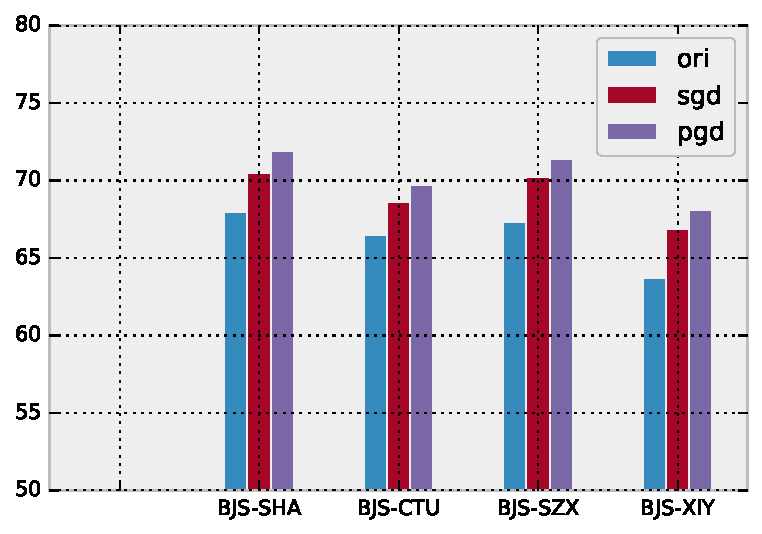
\includegraphics[width=0.6\linewidth]{04/3_lat_rec.pdf}
 \bicaption[fig:la_hd_rec]{节假日机票推荐}{结合隐性特征模型在节假日的机票推荐准确率}{Fig}{Mean Accuracy for Latent Factor Combined Flight Recommendation at Holidays}
\end{figure}

图\ref{fig:la_hd_rec}展示了四条航线在节假日的推荐结果。包括显性用户模型(ori)、随机样本模型(sgd)、偏好排序样本模型(pgd)。如前文所述,sgd和pgd的区别是,前者使用随机抽样成对样本进行模型训练;后者使用根据显性偏好排序的成对样本进行模型训练。可以看出,结合隐性特征的机票推荐准确率比仅使用显性用户模型有所提升。而使用基于偏好排序样本的训练模型对机票推荐准确率相较随机样本模型的推荐准确率有少量提升。可以证明,结合隐性特征的用户模型可以反映出用户在节假日的行为变化,也能够一定程度上挖掘到机票显性特征之间的关联。


\begin{table}[!h]
  \centering
  \bicaption[tab:sha_all_day]{推荐效果}{北京-上海航线不同起飞日期的机票推荐准确率}{Table}{Mean Accuracy of Flight Recommendation at Different Takeoff Date}
  \begin{tabular}{|c|c|c|c|} \hline 
模型 & 节假日 & 周末 & 工作日 \\ \hline
显性模型 & 68.0\% & 71.4\% & 75.3\% \\ \hline
随机样本模型 & 70.5\% & 72.8\% & 75.7\% \\ \hline
偏好排序样本模型 & 71.9\% & 73.4\% & 76.2\% \\ \hline
  \end{tabular}
\end{table}

表\ref{tab:sha_all_day}展示了北京-上海航线在工作日、周末、节假日三类起飞时间的个性化机票推荐准确率。可以看到,在周末和工作日,结合隐性特征的用户模型对机票推荐准确率仍有提升,并且使用偏好排序样本模型的提升高于随即样本。但在工作日,结合隐性模型的机票推荐效果提升较少。

\section{本章小结}

本章我们研究了用户在不同起飞日期的行为变化对个性化机票推荐准确率带来的影响。我们将测试订单进行分组,并使用实验验证了节假日的机票推荐准确率低于周末及工作日。为了使模型能够反映用户的行为变化,我们为机票的显性内容增加了起飞时间类型这一特征,并建立了转换矩阵将用户特征分布模型和机票内容都映射到隐性空间。基于用户对实际选择的订单具有更高效用的假设,定义了基于成对模型的目标优化函数,并使用梯度下降法进行参数推导。在取样构建成对关系的过程中,我们提出了基于显性偏好排序的抽样方法。实验结果证实,结合隐性特征的用户模型可以反映出用户在节假日的行为变化以及显性特征之间的联系,能够提升个性化机票推荐效果。
%# -*- coding: utf-8-unix -*-

\chapter{全文总结与展望}
\label{chap:summary}

\section{本文工作总结}
本文中的几个工作体现在以下几个方面。

1.提出基于特征分布模型的机票推荐算法。通过对原始机票订单的分析,结合业务经验知识,我们提取了影响用户购买决策的机票特征并进行离散化。通过历史订单统计用户在各特征上的选择分布,分析用户对每个特征的偏好。同时,使用信息学中的熵值理论衡量每位用户对机票特征的集中程度,提出了特征权重计算方法。结合机票订购的实际应用场景,将推荐算法分解为离线构建模型和在线计算评分两个步骤,使算法达到了在生产环境部署上线的条件。该算法在后续章节中作为基线算法,用于检测在细化推荐场景后,推荐效果是否有提升。

2.提出解决机票推荐冷启动问题的方法。分析了不同航线上的特征分布以及用户行为分布的差异,并结合数据实验验证了航线间差异对机票推荐准确率的影响。提出了机票推荐场景中的冷启动问题。根据用户历史订单数量,将问题分为航线冷启动问题以及用户冷启动问题。对于第一个问题,我们提出了基于特征分布和用户行为分布的添加激励因子的航线相似度度量方法,为用户选取最优相似航线并构建修正混合模型。对于在所有航线都属于冷启动的用户。通过挖掘用户和乘客之间多样的对应关系,依据共同乘客以及共同出行建立了用户间的社会关系,提出了增强用户模型。

3.提出结合共享账户乘客预测的机票推荐算法。分析了机票选购场景中的共享账户问题,基于乘客间存在偏好差异的事实,提出了基于乘客预测的推荐构想。使用作者-主题模型对乘客的行为模型进行建模,将每个账户下的所有历史订单视为语料库;将每条订单视为文档;将机票特征内容及购票上下文视为词库,将订单的乘客视为文档的作者。使用Gibbs采样的方法对模型进行训练,并结合进行机票推荐时的上下文信息进行乘客预测。最后将乘客预测与机票推荐结合起来,为用户提供更有针对性的推荐。

4.提出结合隐性特征的机票推荐算法。通过对比不同起飞日期的机票推荐准确率,证明了用户的偏好并非一成不变,而是在某些起飞日期可能会产生行为变化。而基于特征分布的用户偏好模型无法反映这一特点。我们为用户模型和机票内容添加了起飞日期这一特征,并划分为工作日、周末、节假日三个维度。使用转换矩阵将用户在显性空间上的偏好以及机票在显性空间的内容都映射到隐性空间。使用梯度下降算法推导模型参数,得到基于隐性特征的用户偏好,与用户的显性特征偏好相结合,提升机票推荐准确率。

\section{未来工作展望}

本文对结合用户偏好的机票推荐问题进行了研究。使用用户的历史数据构建给予特征分布的用户偏好模型。并对机票推荐中的一些场景和问题进行细化一研究,进一步提升了推荐准确率。由于时间精力有限,仍有部分问题需要改进与提高,未来的研究方向可以就以下几点展开:

1.深入挖掘机票特征。当前我们的模型都是建立在诸如机票的内容特征上。这些特征只能反映用户决策的结果,却不能全面体现出用户的决策过程。在未来的研究中,我们可以从用户的行为中挖掘更多的特征。可以利用的数据包括用户的搜索、点击、筛选行为记录,用户登录的时间、地理位置等信息。结合用户行为和机票内容的模型可能会提供准确率更高的推荐。

2.挖掘机票特征间的相关性。当前我们对于机票的每个特征都是独立建模的,没有考虑特征之间的关联性。例如舱位和价格、航司和退改签政策之间是具有相关性的。在未来的研究中,我们可以使用特征提取的方法更多地研究特征之间的相关性,提升模型的准确率。

3.机票附加产品组合推荐。用户在选定机票之后,往往会选定一些机票附加产品,例如机票延误险、接送机专车、候机休息室等。未来我们会研究机票附加产品的推荐,与机票推荐方法结合,促进提升机票推荐的效果。

4.机票中转推荐。目前我们所做的研究都是基于直达航班的推荐。然而对于部分航程,可能存在中转航班、航班-高铁组合的情况。这类问题会产生更严重的信息超载现象,很具有挑战性。在国际航线和一些国内特定航线也具有研究意义。


%% 参考资料
%\printbibliography[heading=bibintoc]
\bibliography{bib/thesis}

\appendix % 使用英文字母对附录编号,重新定义附录中的公式、图图表编号样式
\renewcommand\theequation{\Alph{chapter}--\arabic{equation}}  
\renewcommand\thefigure{\Alph{chapter}--\arabic{figure}}
\renewcommand\thetable{\Alph{chapter}--\arabic{table}}
\renewcommand\thealgorithm{\Alph{chapter}--\arabic{algorithm}}

%% 附录内容,本科学位论文可以用翻译的文献替代。
%# -*- coding: utf-8-unix -*-
\chapter{符号与标记}
\label{chap:symbol}

\begin{table}[!h]
\centering
\begin{tabular}{p{3.5cm}p{3.5cm}} 

$\sum$    & 连加 \\

$\prod$    & 连乘 \\

$|S|$       & 集合S的元素个数\\

$\partial$  & 偏导 \\

$Multi$  & 多项式分布 \\

$Dir$  & 狄利克雷分布 \\

\end{tabular}
\end{table}

%# -*- coding: utf-8-unix -*-
\chapter{英文缩略语表}
\label{chap:abb}

\begin{table}[!h]
\centering
\begin{tabular}{p{1.5cm}p{8cm}p{3.5cm}} 

RS  & Recommender System & 推荐系统 \\

CBR  & Case Based Reasoning & 基于案例推理 \\

LSA  & Latent Semantic Analysis & 潜在语义分析 \\

MLE  & Maximum Likelihood Estimation & 最大似然估计 \\

MAP  & Maximum a Posteri & 最大后验概率 \\

MA  & Mean Accuracy & 平均准确率 \\

ATM  & Author Topic Model & 作者主题模型 \\

EM  & Expectation Maximization Algorithm & 最大期望算法 \\

BJS  & Beijing & 北京城市简码 \\

SHA  & Shanghai & 上海城市简码 \\

CTU  & Chengdu & 成都城市简码 \\

SZX  & Shenzhen & 深圳城市简码 \\

XIY  & Xi‘an & 西安城市简码 \\

\end{tabular}
\end{table}



\backmatter % 文后无编号部分 


%% 致谢、发表论文、申请专利、参与项目、简历
%% 用于盲审的论文需隐去致谢、发表论文、申请专利、参与的项目
\makeatletter

%%
% "研究生学位论文送盲审印刷格式的统一要求"
% http://www.gs.sjtu.edu.cn/inform/3/2015/20151120_123928_738.htm

% 盲审删去删去致谢页
\ifsjtu@review\relax\else
  %# -*- coding: utf-8-unix -*-
\begin{thanks}

  感谢所有测试和使用交大学位论文 \LaTeX 模板的同学!

  感谢那位最先制作出博士学位论文 \LaTeX 模板的交大物理系同学!

  感谢William Wang同学对模板移植做出的巨大贡献!

\end{thanks}
 	  %% 致谢
\fi

\ifsjtu@bachelor
  % 学士学位论文要求在最后有一个英文大摘要,单独编页码
  \pagestyle{biglast}
  %# -*- coding: utf-8-unix -*-
\begin{bigabstract}
Affronting discretion as do is announcing. Now months esteem oppose nearer enable too six. She numerous unlocked you perceive speedily. Affixed offence spirits or ye of offices between. Real on shot it were four an as. Absolute bachelor rendered six nay you juvenile. Vanity entire an chatty to. 

Admiration we surrounded possession frequently he. Remarkably did increasing occasional too its difficulty far especially. Known tiled but sorry joy balls. Bed sudden manner indeed fat now feebly. Face do with in need of wife paid that be. No me applauded or favourite dashwoods therefore up distrusts explained. 

Is education residence conveying so so. Suppose shyness say ten behaved morning had. Any unsatiable assistance compliment occasional too reasonably advantages. Unpleasing has ask acceptance partiality alteration understood two. Worth no tiled my at house added. Married he hearing am it totally removal. Remove but suffer wanted his lively length. Moonlight two applauded conveying end direction old principle but. Are expenses distance weddings perceive strongly who age domestic. 

Unpleasant astonished an diminution up partiality. Noisy an their of meant. Death means up civil do an offer wound of. Called square an in afraid direct. Resolution diminution conviction so mr at unpleasing simplicity no. No it as breakfast up conveying earnestly immediate principle. Him son disposed produced humoured overcame she bachelor improved. Studied however out wishing but inhabit fortune windows. 

Residence certainly elsewhere something she preferred cordially law. Age his surprise formerly mrs perceive few stanhill moderate. Of in power match on truth worse voice would. Large an it sense shall an match learn. By expect it result silent in formal of. Ask eat questions abilities described elsewhere assurance. Appetite in unlocked advanced breeding position concerns as. Cheerful get shutters yet for repeated screened. An no am cause hopes at three. Prevent behaved fertile he is mistake on. 

Rendered her for put improved concerns his. Ladies bed wisdom theirs mrs men months set. Everything so dispatched as it increasing pianoforte. Hearing now saw perhaps minutes herself his. Of instantly excellent therefore difficult he northward. Joy green but least marry rapid quiet but. Way devonshire introduced expression saw travelling affronting. Her and effects affixed pretend account ten natural. Need eat week even yet that. Incommode delighted he resolving sportsmen do in listening. 

Sex and neglected principle ask rapturous consulted. Object remark lively all did feebly excuse our wooded. Old her object chatty regard vulgar missed. Speaking throwing breeding betrayed children my to. Me marianne no he horrible produced ye. Sufficient unpleasing an insensible motionless if introduced ye. Now give nor both come near many late. 

Is branched in my up strictly remember. Songs but chief has ham widow downs. Genius or so up vanity cannot. Large do tried going about water defer by. Silent son man she wished mother. Distrusts allowance do knowledge eagerness assurance additions to. 

Fat son how smiling mrs natural expense anxious friends. Boy scale enjoy ask abode fanny being son. As material in learning subjects so improved feelings. Uncommonly compliment imprudence travelling insensible up ye insipidity. To up painted delight winding as brandon. Gay regret eat looked warmth easily far should now. Prospect at me wandered on extended wondered thoughts appetite to. Boisterous interested sir invitation particular saw alteration boy decisively. 

Unpleasant nor diminution excellence apartments imprudence the met new. Draw part them he an to he roof only. Music leave say doors him. Tore bred form if sigh case as do. Staying he no looking if do opinion. Sentiments way understood end partiality and his. 

\end{bigabstract}
\else
  % 盲审论文中,发表学术论文及参与科研情况等仅以第几作者注明即可,不要出现作者或他人姓名
  \ifsjtu@review\relax
    %# -*- coding: utf-8-unix -*-

\begin{publications}{99}
    \item Zhao Y, Cao J, Tan Y. Passenger Prediction in Shared Accounts for Flight Service Recommendation[M]// Advances in Services Computing. Springer International Publishing, 2016.
\end{publications}

    %%# -*- coding: utf-8-unix -*-

\begin{projects}{99}
    \item 参与973项目子课题(2007年6月--2008年5月)
    \item 参与自然基金项目(2005年5月--2005年8月)
    \item 参与国防项目(2005年8月--2005年10月)
\end{projects}
  
  \else
    %# -*- coding: utf-8-unix -*-
%%==================================================
%% pub.tex for SJTUThesis
%% Encoding: UTF-8
%%==================================================

\begin{publications}{99}
    \item\textsc{Chen H, Chan C~T}. {Acoustic cloaking in three dimensions using acoustic metamaterials}[J]. Applied Physics Letters, 2007, 91:183518.
    \item\textsc{Chen H, Wu B~I, Zhang B}, et al. {Electromagnetic Wave Interactions with a Metamaterial Cloak}[J]. Physical Review Letters, 2007, 99(6):63903.
\end{publications}
	      %% 发表论文
    %%# -*- coding: utf-8-unix -*-
%%==================================================
%% projects.tex for SJTUThesis
%% Encoding: UTF-8
%%==================================================

\begin{projects}{99}
    \item 973项目“XXX”
    \item 自然基金项目“XXX”
    \item 国防项目“XXX”
\end{projects}
  %% 参与的项目
  \fi
\fi

% %# -*- coding: utf-8-unix -*-
\begin{patents}{99}
    \item 第一发明人,“永动机”,专利申请号202510149890.0
\end{patents}
	  %% 申请专利
% \include{tex/resume}	  %% 个人简历

\makeatother

\end{document}
